\chapter{A rede que Marcelo construiu}
\label{capitulo4}

O \enquote{Covideiro} foi o nome que Marcelo usou para designar as enfermarias de pronto-socorro lotadas de pacientes com Covid-19: um ambiente que constitui, nos termos de \textcite{Akrich1992Description}, uma \textit{configuração}, um conjunto de actantes humanos e não humanos onde competências e performances são distribuídas de maneira que nenhum protocolo de coleta poderia ter antecipado. Quando Marcelo decidiu coletar dados nesse ambiente, ele próprio diz que era \enquote{ignorante mais do que louco}: na primeira vez que entrou em uma enfermaria de Covid, disse que \enquote{quase desmaiou}; depois disso, a coleta ficou a cargo de alunos do quarto ano de medicina e de médicos estrangeiros que, por restrições contratuais, só podiam atuar dentro do HC (Hospital das Clínicas da Faculdade de Medicina da Universidade de São Paulo); os médicos internos estavam, nas palavras de Marcelo, \enquote{absolutamente soterrados de trabalho}.\footnote{Em \textit{After Lockdown}, Latour descreve a experiência pandêmica como uma ``metamorfose'' kafkiana: ``é como se eu também tivesse sofrido uma metamorfose real em janeiro de 2020. Ainda me lembro de como, antes, eu podia me mover inocentemente carregando meu corpo comigo. Agora sinto que tenho de me esforçar e carregar nas costas uma longa trilha de CO$_2$ [\ldots] e, pior ainda desde janeiro, porque agora projeto à minha frente (me dizem sem parar) uma nuvem de aerossóis cujas gotículas finas podem espalhar pequenos vírus nos pulmões capazes de matar meus vizinhos'' \textcite[p.~4]{Latour2021AfterLockdown}. Essa ``carapaça de consequências'' que o corpo pandêmico carrega consigo é precisamente o que os coletores encontraram no Covideiro: corpos que projetam aerossóis, tosses, gemidos, que ao mesmo tempo precisam falar ao celular para que a pausa na fala possa ser captada como biomarcador. O vírus não é apenas o ``objeto'' da pesquisa, mas um actante que reconfigura toda a \textit{configuração}: impõe máscaras que fazem barulho, protetores de plástico que distorcem o som, distâncias que enfraquecem o sinal do microfone.} A escolha pelo celular simples, sem cabine de som, sem microfone direcional, sem nenhum dos filtros que os fonoaudiólogos exigem como condição mínima de trabalho, foi, por isso mesmo, uma escolha constitutiva: \enquote{perdi noventa e cinco por cento dos fonoaudiólogos do Brasil}, disse Marcelo, descrevendo a seleção de aliados que o antiprograma do Covideiro impôs. O que restou foi o celular ``porcaria, o que tiver'', o protetor facial e as máscaras que farfalhavam, e a enfermaria reverberando ao fundo. Marcelo descreve esse ambiente:

\begin{citacaoabnt}
Eu sou especialista em lidar com dados ruins. Dados com muito ruído. Coletados no meio de uma enfermaria de Covid, onde a primeira vez que entrei quase desmaiei. Pensei comigo, isso aqui deve ser a maior fonte de ruído que existe. Tinha gente tossindo, gemendo, enfermeiras conversando, televisão ligada, carrinho passando, tudo reverberando sem controle. [\ldots] Usei qualquer celular que tinha em mãos, simples, na pandemia, com máscara e protetor de plástico que fazia barulho. Era isso ou nada, não tinha outra opção (Finger, 2023, informação verbal).
\end{citacaoabnt}

Quem sustentou a presença cotidiana no Covideiro foram os coletores autorizados, alunos do quarto ano de medicina e médicos estrangeiros cujas horas de trabalho dentro do HC permitiam encaixar a coleta dentro dos limites contratuais. Marcelo coordenava de fora. \enquote{Eu não tenho a menor competência pra andar lá paramentado}, disse ele (Finger, 2023, informação verbal). A frase registra uma delegação: o corpo que suportaria o Covideiro seria outro, e o programa de ação do Spira precisou ser reescrito em torno dessa redistribuição. A configuração do Covideiro redistribuiu, nesse sentido, não apenas equipamentos e protocolos, mas os corpos que podiam entrar, e os que permaneciam do lado de fora (além dos corpos doentes). Apesar das dificuldades, Marcelo viu nisso uma oportunidade: \enquote{a pandemia foi o melhor momento da história para coletar dados em processamento de áudio. Por quê? Porque, na época, os hospitais estavam lotados de pacientes. Você podia coletar dados de dez, quinze pacientes em meia hora.}\footnote{Marcelo não descreveu em detalhes a superlotação das alas, mas o problema era que havia mais pacientes do que leitos disponíveis e médicos para atendê-los. A coleta do Spira foi aprovada pelo Comitê de Ética em Pesquisa do Hospital das Clínicas da Faculdade de Medicina da Universidade de São Paulo (CEP-HCFMUSP) em 24 de abril de 2020, antes do início da coleta de pacientes, que os metadados do repositório público situam a partir de 11 de maio de 2020. O protocolo tramitou sob o Código de Identificação CAAE 30918120.0.0000.0068. O consentimento dos participantes foi obtido de forma oral e gravado junto com os dados de áudio, solução aprovada pelo comitê para as condições das enfermarias durante o pico pandêmico, quando a assinatura presencial seria inviável. Os registros formais desse consentimento aparecem em dois pareceres consecutivos do mesmo comitê para o mesmo protocolo: o Parecer~3.988.088, referenciado em \textcite{Berti2023Frequency}, e o Parecer~5.155.306, referenciado em \textcite{Berti2025Healthcare}, o que indica que o estudo passou por ao menos dois ciclos de revisão ética entre 2020 e 2024. Os dados foram completamente anonimizados: o sistema de coleta não registra nenhum dado de identificação pessoal, usando apenas o número de identificação hospitalar, sem acesso ao registro que permitisse a reconexão com o indivíduo \parencite{Finger2025SPIRABM}. Os próprios pesquisadores não sabem quem doou as gravações \parencite{Casanova2021DeepLearning}.}

Entre os aliados que permaneceram ao longo desse processo estava Larissa, professora Dra. do Departamento de Fonoaudiologia da Unesp de Marília. Marcelo a descreveu como alguém que disse \enquote{eu tô junto, Finger, eu tô junto com você}: uma subscrição \parencite{AkrichLatour1992Convenient} feita precisamente nas condições que a maioria recusava. Juntos, Larissa e Marcelo desenvolveram um trabalho sobre a pausa na fala como biomarcador da Covid-19, enquadrado sob a perspectiva de \textit{big data} e \textit{small data} para explicar como a equipe trabalhava com amostras pequenas e ruidosas. O trabalho recebeu o primeiro prêmio no Simpósio Brasileiro de Fonoaudiologia. A parceria com Larissa não foi apenas clínica: ela situou a rede de coleta do Spira em um polo institucional distinto do HC-USP e abriu os hospitais de Marília como sítios de coleta.\footnote{Larissa Cristina Berti é professora doutora do Departamento de Fonoaudiologia da Faculdade de Filosofia e Ciências da Universidade Estadual Paulista (Unesp), campus de Marília. Sua entrada na rede do Spira é registrada, nos artigos, de forma progressiva: aparece primeiro como coautora dos estudos de análise acústica de voz em pacientes com Covid-19 (\textcite{Svartman2022Temporal}, \textcite{Berti2023Frequency}), depois como coautora dos artigos de aprendizado de máquina (\textcite{Gauy2024Discriminant}) e, finalmente, como autora correspondente do artigo sobre características acústicas em pós-Covid (\textcite{Berti2025Healthcare}) e membro central da equipe do Spira-BM (\textcite{Finger2025SPIRABM}). O CNPq inscreve essa trajetória individualmente: Berti aparece com bolsa de produtividade própria (301735/2019-0, renovada como 304961/2021-3) nos artigos de fonética e fonoaudiologia, o que a distingue dos pesquisadores do núcleo de NLP do IME-USP, cujo financiamento individual pelo CNPq é de Finger como único pesquisador de produtividade identificável na série. Essa dupla inscrição, pelo auxílio coletivo da Fapesp e pela bolsa individual do CNPq, é a forma pela qual os artigos registram que Larissa pertence à rede do Spira sem pertencer ao laboratório de Marcelo: ela é uma aliada com financiamento e institucionalidade próprios, e é precisamente essa autonomia que a torna um actante de continuidade entre as duas fases do projeto. A Unesp de Marília, por sua vez, não é apenas uma filiação: é a instituição que viabilizou o acesso aos quatro hospitais da cidade, conectando a rede de coleta de P2 a um polo institucional cujas relações com os estabelecimentos de saúde de Marília precediam e excediam o projeto Spira. Quando Marcelo descreve Larissa como alguém que ``ficou junto'', o que o agradecimento nos artigos registra, nos termos de \textcite{LatourMauguinTeil1992}, é um movimento paradigmático: o papel do fonoaudiólogo permaneceu inscrito na configuração, e o que se alterou foi o perfil de actante recrutável para habitá-lo nas condições do Covideiro.}

Os artigos científicos, por exemplo, mencionam a necessidade de adicionar \enquote{ruídos de enfermaria hospitalar tanto aos áudios dos pacientes quanto aos controles de não pacientes coletados de aplicativos na internet} para evitar o sobreajuste dos modelos.\footnote{Sobreajuste (\textit{overfitting}) designa o fenômeno em que um modelo de aprendizado de máquina aprende os padrões específicos dos dados de treinamento com precisão tão elevada que perde a capacidade de generalizar para dados novos. Em vez de extrair as regularidades que definem o fenômeno de interesse, o modelo memoriza as particularidades do conjunto com que foi treinado, incluindo características que nada têm a ver com o que se quer detectar. No caso do Spira, o risco concreto era que o modelo aprendesse a associar ausência de ruído de fundo a saúde e presença de ruído a doença, porque os controles saudáveis foram coletados em ambientes domésticos silenciosos e os pacientes, em enfermaria hospitalar. A adição artificial de ruído de enfermaria aos áudios de controle é a resposta técnica a esse antiprograma: força o modelo a aprender a diferença entre os dois grupos a partir do sinal de fala e não do ambiente acústico.} Os diferentes ambientes de coleta exigem pré-processamento para que o modelo não aprenda os ruídos como características distintivas da doença. Os detalhes técnicos da amostra \textcite{Gauy2024Discriminant} incluíram: 26 pacientes com insuficiência reSpiratória (14 homens, 12 mulheres; duração média: 8,14s) e 116 controles (36 homens, 80 mulheres; duração média: 7,41s); áudios amostrados a 16kHz; 128 coeficientes MFCC (\textit{Mel-Frequency Cepstral Coefficients}); dados coletados em 4 hospitais: Beneficência Portuguesa, Hospital da Unimar, Santa Casa de Marília e CEES-Marília.\footnote{A coleta de P2 nos quatro hospitais de Marília corresponde à expansão clínica do projeto para insuficiência reSpiratória de causas diversas, em período pós-pandêmico. Essa expansão exigiu um segundo protocolo de aprovação: o CAAE 85388624.0.0000.0068, submetido ao CEP-HCFMUSP e à Plataforma Brasil, o sistema nacional de revisão ética em pesquisa com seres humanos \parencite{Finger2025SPIRABM}. A existência de dois CAEEs para o mesmo projeto registra a transição do Spira de intervenção emergencial pandêmica a programa de pesquisa clínica sistemática: o protocolo original (CAAE 30918120.0.0000.0068) fora aprovado em abril de 2020 em ritmo acelerado pela urgência sanitária; o protocolo da segunda fase percorreu o circuito completo da avaliação nacional, incluindo a Plataforma Brasil, instância que o protocolo original não havia acionado. Essa diferença de percurso regulatório é, por si só, um rastro do que a emergência pandêmica havia tornado possível e do que a rotina do pós-pandemia reinstalava como condição.}

Os quatro sítios de coleta marcam a extensão geográfica da rede. Os quatro hospitais de Marília conectam-se diretamente à parceria com Larissa: foi o polo da Unesp que viabilizou o acesso a esses ambientes clínicos. A dispersão por múltiplos sítios é, ao mesmo tempo, uma ampliação da cadeia de inscrição e uma resposta ao antiprograma do Covideiro: ao distribuir a coleta por ambientes institucionais heterogêneos, a equipe aumentava a diversidade acústica das amostras. Os experimentos de ruído do primeiro artigo \parencite{Casanova2021DeepLearning} mostram por que essa diversidade era operante para a generalização: sem nenhum ruído, o modelo atingia 98,15\% de acurácia no teste limpo e caía para 50,93\% quando se introduzia ruído no teste, sinal de que o que ele aprendera era o silêncio do laboratório, e não a assinatura acústica da insuficiência reSpiratória; ao se adicionar ruído de paciente e de controle de forma progressiva, a acurácia subia até um pico, com três amostras de cada, e degradava depois, quando o sistema deixava de distinguir sinal de antiprograma.

O estudo utilizou redes neurais de áudio pré-treinadas (CNN6, CNN10, CNN14) e o \textit{Autoencoder} Mascarado (Audio-MAE), que combinados alcançaram precisão de 96,5\% na detecção da insuficiência reSpiratória.\footnote{As redes pré-treinadas utilizadas pelo Spira constituem, nos termos de \textcite{Latour2011CienciaEmAcao}, \textit{caixas-pretas}: dispositivos cujo funcionamento interno não precisa ser reaberto a cada uso. A CNN14, por exemplo, foi treinada com o dataset AudioSet (mais de 5.000 horas de áudio etiquetado do YouTube), corpus do Google composto majoritariamente de conteúdo extraído da plataforma, e transportada para o contexto do Spira sem que seus parâmetros internos fossem reexaminados: milhões de pesos sinápticos ajustados em outro contexto são aceitos como estáveis e reutilizáveis. O conceito de caixa-preta é aqui literal: o artigo menciona 80 milhões de parâmetros (CNN14), mas não reabre a questão de como esses parâmetros foram ajustados. Reabrir essa caixa-preta exigiria mobilizar recursos equivalentes aos que foram necessários para fechá-la, o que, neste caso, significaria dispor de milhares de horas de áudio e capacidade computacional equivalente à do Google Research. O Audio-MAE percorre um trajeto distinto: desenvolvido pelo Meta AI Research, é um \textit{autoencoder} mascarado que aprende por auto-supervisão, sem rótulos humanos, construindo representações acústicas a partir da tarefa de reconstruir espectrogramas com partes mascaradas. Os dois modelos chegam ao Spira como caixas-pretas fechadas em centros de cálculo distintos, com lógicas de produção irredutíveis entre si: supervisão etiquetada por humanos sobre 527 categorias sonoras, de um lado; auto-supervisão sobre a estrutura acústica dos sinais, de outro. Da mesma forma, os 128 coeficientes MFCC funcionam como caixa-preta consolidada: o artigo aplica a transformação sem justificá-la, porque ela já está estabilizada como prática padrão no campo de processamento de áudio.} O enunciado ``96,5\% de precisão'' ocupa, na estrutura do artigo, uma posição que \textcite{Latour2011CienciaEmAcao} descreveria como desmodalizada: apresenta-se sem as condições de sua produção, como se os dados ``falassem por si'' e a natureza se revelasse diretamente nos coeficientes MFCC. É o enunciado que pode ser citado por outros artigos sem passar pela seção de métodos; pode aparecer em relatórios institucionais e pedidos de financiamento como ``o Spira detecta IR com 96,5\% de precisão'', frase que, em seu percurso, foi progressivamente desligada do Covideiro pandêmico de São Paulo, dos três hospitais onde a coleta ocorreu, dos celulares baratos e do ruído controlado artificialmente que a tornaram possível. A \textit{imagem de Janus} \parencite{Latour2011CienciaEmAcao}\footnote{Latour utiliza a figura na abertura de \textit{Ciência em ação} sem desenvolver a referência mitológica: apresenta as duas faces como dispositivo visual e analítico, deixando ao leitor a tarefa de reconhecer a aptidão do nome. Para o leitor menos familiarizado com a mitologia romana, vale a contextualização: Janus é o deus das passagens, das portas e das transições, e sua iconografia canônica é a de duas faces opostas, uma voltada para frente e outra para trás. A pertinência da figura para o argumento de Latour reside precisamente nessa geometria: o que determina qual face do objeto científico aparece não é o objeto em si, mas o momento em que o observador chega. Quem acompanha o laboratório antes do fechamento da caixa-preta encontra a ciência em construção, com suas controvérsias, escolhas técnicas e condições de produção ainda visíveis; quem chega depois encontra a natureza ``falando por si'', o fato estabilizado sem as marcas de sua produção. O uso da figura excede, assim, o registro puramente metafórico: ela organiza o método inteiro de \textit{Ciência em ação}, que propõe seguir cientistas e engenheiros \textit{antes} que os fatos se fechem. No caso do Spira, as duas faces são o artigo que reporta 96,5\% de precisão e a entrevista com Marcelo que restituiu o Covideiro, os fonoaudiólogos perdidos e o ruído artificialmente adicionado.} orienta a leitura desse momento: quando o artigo apresenta a precisão de 96,5\%, está na face ``realista'' de Janus, os dados falam por si, o modelo detecta a insuficiência reSpiratória, a natureza revela seus padrões acústicos. O enunciado desmodalizado é o que pode circular como fato.

Contudo, limitações importantes persistem. Em primeiro lugar, a estimativa de SpO$_2$: ``os modelos apresentam valores de erro quadrático médio que excedem a faixa clínica aceita de 3,5\% para oxímetros de dedo''\footnote{O erro quadrático médio (\textit{Root Mean Squared Error}, RMSE) mede a distância média entre os valores previstos pelo modelo e os valores reais medidos, expressa na mesma unidade da variável: no caso, pontos percentuais de SpO$_2$. A faixa de 3,5\% é o padrão estabelecido para uso clínico de oxímetros de dedo \parencite{Gauy2025Contrasting}. Os oxímetros convencionais apresentam erro típico entre 1\% e 2\% \parencite{Gauy2025Contrasting}. Os quatro modelos testados pelo Spira atingiram RMSE entre 4,4 e 4,8, todos acima do limiar clínico, com o melhor erro absoluto médio em torno de 3,0 pontos percentuais \parencite{Gauy2025Contrasting}.} e ``os coeficientes de correlação de Pearson não ultrapassam 0,3''\footnote{O coeficiente de correlação de Pearson mede o grau de associação linear entre dois conjuntos de valores, em uma escala de $-1$ a $+1$: valores próximos de $+1$ indicam que as duas variáveis variam juntas de modo previsível; valores próximos de 0 indicam ausência de associação linear. Os modelos testados atingiram Pearson entre 0,03 e 0,25, indicando que os valores de SpO$_2$ previstos pela voz têm associação muito fraca com os valores registrados pelo oxímetro \parencite{Gauy2025Contrasting}. Os próprios autores interpretam esse resultado como evidência de que a voz contém informações sobre a presença de insuficiência reSpiratória, mas não sobre o nível de saturação de oxigênio em si \parencite{Gauy2025Contrasting}.} \parencite{Gauy2024Discriminant}. 
Em segundo, a generalização limitada: ``os modelos treinados com dados de P1 [Covid-19] não se aplicam bem a P2 [insuficiência reSpiratória de diferentes causas], sugerindo que a insuficiência reSpiratória causada pela Covid-19 tem características que podem ser diferentes das de outras causas'' \parencite{Gauy2024Discriminant}. Os próprios autores acrescentam, na seção de resultados: ``P2 is not harder, it is only different'' \parencite{Gauy2024Discriminant}. A distinção entre dificuldade e diferença organiza a leitura de toda esta seção: porque P2 é diferente, o modelo é circunscrito, e não deficiente; um modelo apenas mais exigido pela dificuldade de P2 seria tecnicamente insuficiente, ao passo que um modelo que encontra em P2 outro objeto é um modelo que cumpriu o que a rede o construiu para fazer e alcançou o limite dessa construção. Ao formular a diferença, o artigo re-modaliza o enunciado de 96,5\%, devolve à visibilidade as condições de produção que esse resultado havia apagado. A face ``relativista'' de Janus reaparece: os autores mobilizam cautelas, qualificações e ressalvas que revelam o trabalho de construção por trás do resultado.\footnote{A franqueza das limitações é, ela própria, uma estratégia retórica que Latour identifica em \textit{Ciência em Ação}: a seção de limitações de um artigo científico funciona como um escudo. Ao antecipar as objeções mais óbvias e enquadrá-las como reconhecimento honesto, o artigo dificulta que os contestadores as usem como argumento de refutação. A seção de limitações do artigo do Spira, ao declarar explicitamente que os modelos não generalizam para IR de outras causas, captura essa objeção e a devolve como conhecimento produzido pelo próprio projeto, ao invés de deixá-la disponível como ataque externo. O que poderia ser a abertura de uma controvérsia torna-se parte do argumento.} É nessa variação entre os dois estados do mesmo enunciado que a insuficiência reSpiratória detectada pelo Spira não conseguiu se estabilizar como \textit{matter of fact} \parencite{latour2004politics}: permanece o \textit{matter of concern}, atada às condições específicas do Covideiro. Em terceiro, após a pandemia surgiu um novo desafio de coleta:

\begin{citacaoabnt}
Se você quer coletar dados para casos de insuficiência reSpiratória, tem que esperar o paciente aparecer. Aparece um, depois três horas outro, depois dois dias sem ninguém, e assim por diante. Então, preciso criar um novo método de coleta (Finger, 2023, informação verbal).
\end{citacaoabnt}

Em conclusão, os artigos científicos do Spira registram que ``a análise de áudio oferece percepções sobre o estado de IR de um paciente, mas não fornece informações precisas sobre os níveis reais de SpO$_2$, indicando uma separação de domínios nos quais biomarcadores de voz e fala podem ou não ser úteis em diagnósticos médicos com as tecnologias atuais'' \parencite{Gauy2025Contrasting}. O resultado é legível, nos termos de \textcite{mol2002body}, como uma multiplicidade ontológica em operação: o SpO$_2$ que o oxímetro de dedo performa, medindo a absorção de luz infravermelha pela hemoglobina no sangue capilar, e o SpO$_2$ que a voz deveria codificar acusticamente são dois objetos produzidos por práticas distintas que o algoritmo não consegue reunir em um único espaço de representação. Mol demonstrou o mesmo fenômeno para a aterosclerose no Hospital de Heerlen: a aterosclerose que o angiograma visualiza nas artérias, a que o Doppler mede como pressão no tornozelo e a que o patologista examina na lâmina histológica são objetos que coexistem sem hierarquia ontológica, sem que nenhum deles seja mais real do que os outros \parencite{mol2002body}. No Spira, o experimento de estimativa de SpO$_2$ expõe a mesma multiplicidade: não há um único objeto ``nível de saturação de oxigênio'' que oxímetro e microfone medem por vias diferentes; há dois objetos distintos que as práticas de cada dispositivo performam. O que o resultado desfaz é a pré-inscrição que o projeto carregava: a suposição de que a pausa na fala, definida como biomarcador da IR, codificaria o SpO$_2$ de modo suficientemente estável para que um modelo aprendesse a ler um através do outro. Nos termos de Latour, o artigo re-modaliza o enunciado mais amplo sobre biomarcadores de voz: o que estava em vias de se tornar fato revela-se proposição situada, válida para um domínio e inoperante em outro \parencite{Latour2011CienciaEmAcao}.

A visão que Marcelo articula para a IA ao final da entrevista funciona, nos termos de \textcite{Akrich1992Description}, como uma pré-inscrição: a descrição do usuário e do contexto que o dispositivo pressupõe para funcionar como ele imagina que deveria funcionar.

\begin{citacaoabnt}
A inteligência artificial pode ser muito útil se ela for usada para suprir nossas deficiências e para complementar as pessoas e resolver problemas. Não para substituir ou descartar, mas para ajudar (Finger, 2023, informação verbal).
\end{citacaoabnt}

O exemplo que ele oferece em seguida é preciso: o Spira em um celular, funcionando no ambulatório do HC e também em uma barca no Rio Tapajós. ``Tem alguém passando mal? Fala aí uma frase, eu falo uma frase, tá com insuficiência reSpiratória, faz alguma coisa com ele, sabe? Te dá um encaminhamento barato'' (Finger, 2023, informação verbal). A barca no Rio Tapajós é o actante que ancora a pré-inscrição do usuário ideal: alguém geograficamente distante do sistema de saúde convencional, sem acesso a equipamento médico, mas com um celular na mão. O celular, nas palavras de Marcelo, ``hoje em dia é \textit{commodity}, todo mundo tem'' (Finger, 2023, informação verbal): a premissa que ancora a visão é a de que o instrumento de coleta já está distribuído, e seu custo não se compara ao do equipamento médico convencional. Essa visão encontrou respaldo técnico no Spira-BM, que a análise dos artigos e do documento de descrição do projeto permite reconstruir como cadeia de inscrições em andamento: a arquitetura da segunda fase prevê explicitamente que dispositivos móveis sejam usados tanto na coleta quanto na avaliação do biomarcador pelo paciente em campo, com processamento possível na nuvem ou no próprio aparelho \parencite{Finger2025SPIRABM}. A pré-inscrição do Tapajós é o horizonte que Marcelo formula como visão na entrevista e que a segunda fase inscreve como arquitetura nos artigos; o Spira-BM como projeto institucionalizado, com suas linhas de pesquisa, seus hospitais e seus financiamentos específicos, não foi descrito por Marcelo na entrevista de 2023 e chegou a esta análise pelo percurso da cadeia textual, seguindo as referências cruzadas dos artigos do Spira original até o documento de descrição do projeto. O antiprograma que se interpõe entre a visão e o dispositivo atual é o que os artigos do Spira original documentam como falha de generalização: o modelo treinado no Covideiro com pacientes Covid-19 aprendeu uma versão da IR acusticamente específica a esse contexto, e a barca no Tapajós exigiria um modelo que reconhecesse IR de causas diversas, em condições acústicas que a pandemia não produziu em quantidade suficiente para treinar. O Spira-BM tenta recrutar esses novos aliados, expandindo a coleta para asma grave e tabagismo em múltiplos hospitais; a questão em aberto, no momento da entrevista, era se o novo contexto de coleta, disperso e lento, conseguiria produzir o volume de dados que o Covideiro pandêmico havia concentrado em meia hora de enfermaria.\footnote{A comparação que Marcelo mobiliza para situar a IA na história das tecnologias é a escrita: ``a escrita tá aí até hoje, acho que foi uma bela e muito mais revolucionária que qualquer inteligência artificial na minha opinião. Mas por muito tempo era uma tecnologia limitada, né? O pessoal era tudo analfabeto'' (Finger, 2023, informação verbal). A analogia situa a IA no registro das tecnologias de externalização cognitiva, aquelas que suprem o que a ``cabeça não conseguia reter'', e condiciona o julgamento sobre seu valor ao critério de acesso. Uma tecnologia de escrita restrita a uma elite de alfabetizados retém seu potencial sem realizá-lo; o mesmo critério se aplica à IA \parencite{Latour2011CienciaEmAcao}.}

A entrevista registra também uma reflexão sobre ética que desloca a visão instrumental para um território mais tenso. Marcelo descreve a responsabilidade do pesquisador de IA nos termos de quem está ``na linha de frente'': o programador que, na hora de escrever uma linha de código, decide se inclui ou não um dado, se um CEP vai produzir discriminação por região, se um sistema de classificação vai punir quem mora em determinado bairro pelo histórico coletivo de seus vizinhos. ``Você faz um erro novo e não sabia, que não sei o que. É uma história. Agora, se você faz um erro velho, aí já é incompetência'' (Finger, 2023, informação verbal). Essa formulação situa a responsabilidade ética na decisão técnica concreta, incidindo sobre o código e sobre os dados antes de qualquer deliberação filosófica abstrata. O que esse posicionamento revela, nos termos de \textcite{Akrich1992Description}, é uma circunscrição do campo de responsabilidade: Marcelo traça o limite entre o que cabe ao pesquisador decidir e o que cabe à sociedade. ``Quem decide é a sociedade'', repete ele, ao discutir os limites do uso de dados de voz para fins pelos quais o paciente não deu consentimento.\footnote{O ``CEP'' a que Marcelo se refere na entrevista é o Código de Endereçamento Postal, e não o Comitê de Ética em Pesquisa: o argumento é que incluir o CEP postal como variável preditiva pode fazer um algoritmo discriminar pessoas pela região em que vivem, penalizando-as pelo histórico coletivo de seus vizinhos em vez de por sua conduta individual. Esse é um exemplo estabelecido de viés geográfico em sistemas de classificação automatizada. No vocabulário da regulação da pesquisa com seres humanos no Brasil, ``o CEP'' designa os comitês institucionais que avaliam e aprovam protocolos, regulamentados pela Resolução CNS~466/2012. A homonímia entre os dois usos delimita dois regimes de responsabilidade que Marcelo articula sem os confundir: o CEP-comitê aprovou o protocolo de coleta do Spira (CAAE 30918120.0.0000.0068, CEP-HCFMUSP, abril de 2020) e circunscreveu os fins declarados do uso das vozes; o CEP-postal é a variável que o programador decide incluir ou excluir no modelo, em uma camada de escolha técnica que o protocolo aprovado pelo comitê raramente especifica com o grau de detalhe que as consequências discriminatórias exigiriam. São dois pontos distintos da cadeia de translações em que a responsabilidade ética se distribui: o comitê age no momento da aprovação do protocolo, o programador age no momento da escrita do código.} O pesquisador que conhece o problema tem a obrigação de sinalizá-lo; a decisão sobre o que pode e o que não pode é da sociedade. É uma divisão de trabalho que inscreve o cientista da computação como ator informado e responsável, sem atribuir a ele o papel de árbitro final das consequências do que produz. O que Marcelo imagina que o Spira deveria fazer, levar a escuta clínica ao Rio Tapajós por celular, é o inverso do que a falha de generalização revelou que ele faz: um dispositivo circunscrito ao Covideiro pandêmico, cujos limites o próprio artigo registra como limitação técnica e que a análise sócio-semiótica lê como a forma que a negociação entre programa e antiprogramas deixou impressa no objeto.

Os dados emergem como elemento central no discurso tecnocientífico formal sobre IA: são o ``alimento'' essencial para sistemas de aprendizado de máquina, permitindo que algoritmos identifiquem padrões, classifiquem, tomem decisões e façam previsões.\footnote{Uma discussão sobre a origem, os tipos e os problemas dos dados para treinamento de modelos de IA, incluindo a distinção entre dados estruturados e não estruturados, as questões de granularidade, privacidade e concentração geográfica no Norte Global, está disponível em \textcite{Helanski2025Dados}, artigo de divulgação científica da autora publicado na plataforma \textit{Understanding Artificial Intelligence} (UAI/IEA-USP). Disponível em: \url{https://understandingai.iea.usp.br/nota-critica/de-onde-vem-os-dados-para-treinar-modelos-de-inteligencia-artificial/}. Acesso em: 29~mar.~2026.} Ao mesmo tempo, constituem um dos aspectos mais polêmicos quando se fala em IA; a própria palavra ``dados'' (\textit{data}, do latim \textit{datum}, ``o que é dado'') já carrega uma pressuposição epistemológica que Latour reinterpreta. Em \textit{A esperança de Pandora}, ao acompanhar pedólogos na floresta amazônica, Latour propõe que ``nunca se deve falar em \textit{data}, ou seja, aquilo que é dado, mas antes em \textit{sublata}, ou seja, aquilo que é `realizado'\,'' \textcite[p.~42]{Latour2017Esperanca}. Desse modo, os ``dados de áudio'' coletados no Covideiro são \textit{realizados} por uma cadeia de decisões, desde a escolha do celular, a instrução ao paciente para repetir frases específicas que induzam pausas, a posição do microfone em relação à máscara, a adição posterior de ruídos de enfermaria aos controles. Cada uma dessas operações é, nos termos de Latour, uma \textit{transformação} que simultaneamente preserva e deforma o fenômeno original.

De onde vêm, concretamente, os dados do Spira? A pergunta parece simples, mas a resposta desdobra a cadeia de realizações que o conceito de \textit{sublata} exige. O dataset utilizado nos estudos do Spira é composto por dois grupos: pacientes hospitalizados com Covid-19 e insuficiência reSpiratória confirmada, recrutados em três hospitais de São Paulo durante a primeira onda da pandemia,\footnote{Os artigos do projeto variam na descrição dos sítios de coleta de P1. \textcite{Casanova2021DeepLearning}, o primeiro artigo publicado, não especifica os hospitais. \textcite{Berti2023Frequency} descreve três hospitais de São Paulo: dois públicos vinculados à Universidade de São Paulo (Hospital das Clínicas da FMUSP e Hospital Universitário) e um privado (Beneficência Portuguesa). A coleta ocorreu entre maio e julho de 2020, com o período dos pacientes compreendido entre 11 de maio e 17 de junho, conforme os metadados do repositório \parencite{Casanova2021DeepLearning}. Os experimentos de aprendizado de máquina dos artigos posteriores utilizaram subconjuntos distintos desses dados, e em \textcite{Gauy2024Discriminant} o foco recai sobre P2, coletado nos quatro hospitais de Marília; a variação nas descrições dos sítios de coleta ao longo da série de artigos reflete essa diferença de escopo experimental.} e um grupo de controle formado por indivíduos saudáveis, sem histórico de comprometimento reSpiratório, recrutados por meio de uma aplicação web \parencite{Casanova2021DeepLearning, Gauy2024Discriminant}. O protocolo de coleta previa três enunciados para cada doador: uma frase de 31 sílabas elaborada por linguistas para induzir pausas reSpiratórias espontâneas e acessível a doadores de baixa escolaridade, ``O amor ao próximo ajuda a enfrentar o coronavírus com a força que a gente precisa''; uma cantiga infantil amplamente conhecida, prevista para doadores com dificuldades de leitura por falta de óculos ou outros impedimentos, ``Batatinha quando nasce, espalha a rama pelo chão, nenezinho quando dorme põe a mão ao coração''; e uma canção do repertório oral comum, ``Parabéns a você, nesta data querida, muitas felicidades, muitos anos de vida'', que dispensava leitura por pertencer à memória coletiva.\footnote{A escolha dos enunciados revela as pré-inscrições do dispositivo sobre seus usuários: doadores que podem não ter óculos na enfermaria, que podem ser analfabetos funcionais, que podem não conseguir ler uma frase em uma tela sob condições de estresse físico. As cantigas infantis e a música de aniversário são actantes recrutados precisamente porque pertencem à memória oral e dispensam leitura. Nos experimentos finais publicados por \textcite{Gauy2024Discriminant}, apenas o primeiro enunciado foi retido para análise, após balanceamento da amostra por classe e sexo: a cantiga e a música desapareceram do artigo, mas estiveram presentes na configuração do Covideiro.} O conjunto está disponível publicamente sob licença Creative Commons (CC~BY-SA~4.0) \parencite{Casanova2021DeepLearning}, e foi a partir de uma amostra desse repositório que gerei os espectrogramas mel apresentados nas figuras da seção seguinte.\footnote{O dataset está hospedado em \url{https://github.com/Spirabr/Spira-audios} (CC~BY-SA~4.0). O repositório contém 219 gravações de pacientes e 213 de controles, distribuídas em partições de treino, avaliação e teste. Esse total difere das cifras reportadas nos artigos do projeto porque os experimentos publicados utilizaram subconjuntos balanceados por classe e sexo: \textcite{Gauy2024Discriminant}, por exemplo, analisou, para o experimento P2, 26 pacientes e 116 controles após balanceamento e reclassificação de dois controles cujo SpO$_2$ estava abaixo do limiar. Os quatro hospitais de coleta de P2, Beneficência Portuguesa, Hospital da Unimar, Santa Casa de Marília e CEES-Marília, são hospitais de Marília e diferem dos três hospitais de São Paulo onde os dados de P1 (Covid-19) foram coletados em 2020 \parencite{Gauy2024Discriminant}. O percurso de acesso ao repositório e de geração dos espectrogramas está documentado na Seção~\ref{sec:nota-llm} e no repositório público \url{https://github.com/julianehelanski/Spira-espectrogramas}.} Acessar essas gravações foi um dos momentos em que a pesquisa deixou de ser análise de artigos científicos e se tornou um encontro com o que os artigos haviam apagado. Ouvir pacientes hospitalizados, com reSpiração entrecortada e voz visivelmente comprometida, recitar a frase sobre o amor ao próximo ou entoar a cantiga da batatinha em uma enfermaria de Covid-19 em pleno maio de 2020 produz algo que nenhuma tabela de metadados do excel antecipa, a presença (ou melhor a ausência) de pessoas e seus sofrimentos que tornaram possível o \textit{dataset} existir. E é precisamente essa presença que a anonimização, condição estrutural da publicação como dado aberto, tornou irrecuperável \parencite{Casanova2021DeepLearning}. Os arquivos dos dois grupos foram anonimizados por mecanismos distintos, inscritos nos próprios nomes dos arquivos. Os controles receberam identificadores UUID gerados automaticamente pela aplicação web no momento da coleta (como \texttt{29f8a854-4072-4379-b0f4-686b49a03c7e\_1.wav}), apagando a identidade desde a origem; os pacientes chegaram pelo \texttt{WhatsApp} e seus arquivos preservam apenas o rastro temporal da transmissão (como \texttt{PTT-20200511-WA0018.wav}), sem que qualquer informação permita identificar o remetente.\footnote{A diferença entre as duas arquiteturas de anonimização é ela própria um dado sobre os dispositivos de coleta: a aplicação web gerou anonimato por design, enquanto o \texttt{WhatsApp} exigiu a remoção posterior do remetente, preservando a data e a hora como único vestígio do ato de envio. O nome do arquivo \texttt{PTT-20200511-WA0018.wav} ainda guarda o dia 11 de maio de 2020 e o número de ordem da mensagem na conversa, rastros do percurso que a des-crição \parencite{Akrich1992Description} consegue recuperar, mas que nada revelam sobre quem falou. A impossibilidade de nomear a voz não é, portanto, apenas questão ética: é, nos termos de \textcite{Latour2017Esperanca}, o preço da mobilidade. Para que a voz viajasse do celular ao repositório, do repositório ao modelo e do modelo ao artigo, ela precisou deixar para trás tudo o que a tornava de alguém.} A anonimização foi, desse modo, uma operação não homogênea mas que foi aplicada uniformemente ao \textit{dataset}, e que foi inscrita de formas distintas em cada grupo, conforme o dispositivo de coleta que cada um utilizou, e essa distinção é legível nos metadados para quem acessa o repositório.

A Tabela~\ref{tab:dataset_Spira} sintetiza a composição do conjunto de dados a partir dos metadados do repositório público, distribuídos em três partições de treino, avaliação e teste.

\begin{table}[!htbp]
\centering
\caption[Composição do dataset Spira: distribuição demográfica, período de coleta e nível de dispneia.]{Composição do dataset Spira: distribuição demográfica, período de coleta e nível de dispneia nos grupos de pacientes e controles. Fonte: metadados do repositório público \url{https://github.com/Spirabr/Spira-audios} (CC~BY-SA~4.0).}
\label{tab:dataset_Spira}
\small
\begin{tabular}{lcc}
\toprule
\textit{Característica} & \textit{Pacientes (classe~1)} & \textit{Controles (classe~0)} \\
\midrule
Total de gravações & 219 & 213 \\
Período de coleta & 11~mai.--17~jun.~2020\footnote{A aprovação do protocolo de ética pelo CEP-HCFMUSP data de 24 de abril de 2020 (CAAE 30918120.0.0000.0068), 17 dias antes do início da coleta de pacientes. A emergência pandêmica acelerou o rito regulatório sem dispensá-lo. O consentimento foi obtido de forma oral e gravado junto com cada áudio, sob o Parecer~3.988.088 \parencite{Berti2023Frequency}; um segundo ciclo de revisão do mesmo protocolo produziu o Parecer~5.155.306 \parencite{Berti2025Healthcare}. A coleta de controles (grupo sem IR, recrutado por aplicativo web) ocorreu entre maio e julho de 2020, com sobreposição ao período dos pacientes \parencite{Casanova2021DeepLearning}.} & mai.--jul.~2020 \\
Canal de coleta & \texttt{WhatsApp} (enfermaria) & Aplicação web (doméstico) \\
\midrule
\textit{Nível de dispneia} & & \\
\quad Nível~5 (máximo) & 219~(100\%) & --- \\
\quad Nível~1 (leve) & --- & 11~(5,2\%) \\
\quad Nível~0 (ausente) & --- & 202~(94,8\%) \\
\midrule
\textit{Sexo} & & \\
\quad Masculino & 119~(54,3\%) & 89~(41,8\%) \\
\quad Feminino & 100~(45,7\%) & 124~(58,2\%) \\
\midrule
\textit{Idade} & & \\
\quad Mínima / máxima & 19 / 90~anos & 18 / 83~anos \\
\quad Média & 53,0~anos & 43,8~anos \\
\quad Faixa predominante & 46--60~anos (41,6\%) & 18--45~anos (54,0\%) \\
\bottomrule
\end{tabular}
\end{table}

A leitura da tabela revela duas disparidades que os artigos formulam tecnicamente mas não desenvolvem em suas implicações ontológicas. A primeira diz respeito ao nível de \textit{dispneia}, termo médico que designa a sensação subjetiva de falta de ar ou dificuldade para reSpirar.\footnote{A coluna \enquote{nivel_falta_de_ar} do dataset registra o grau subjetivo de dificuldade reSpiratória relatado pelo paciente ou aferido no momento da coleta, em uma escala de 0 (ausente) a 5 (máximo). Pacientes com IR por Covid-19 têm dificuldade grave para reSpirar, e é essa dificuldade que altera a textura acústica da fala e produz as pausas que o modelo aprende a reconhecer. A dispneia é, literalmente, o que o espectrograma inscreve como bandas escuras, conforme elaborado na seção \ref{sec:inscricoes_tecnocientificas}.} O dataset não identifica gradações de insuficiência reSpiratória e, por isso, captura um contraste binário extremo entre comprometimento máximo e ausência de comprometimento. Essa configuração é a condição de possibilidade dos 96,5\% de acurácia em P1 e, ao mesmo tempo, a condição de impossibilidade de generalização para P2: quando testado sobre pacientes com insuficiência reSpiratória de outras doenças, onde a dispneia se apresenta em graus intermediários que o Covideiro pandêmico jamais inscreveu no dataset, o modelo perde a fronteira que aprendeu \parencite{Gauy2024Discriminant}. O modelo aprendeu a fronteira inscrita no dataset, e essa fronteira pertencia ao Covideiro, não à condição clínica em sua extensão geral. O que os artigos descrevem como ``detecção de insuficiência reSpiratória por Covid-19'' é, portanto, o resultado de uma cadeia de realizações (\textit{sublata}) que produziu uma versão muito específica dessa condição: a que o Covideiro pandêmico tornou possível, com aquelas pessoas, naqueles 38 dias, naquelas enfermarias \parencite{Gauy2024Discriminant}.

O limiar operacional que separa os dois grupos, saturação de oxigênio igual ou inferior a 92\%, transforma uma condição clínica fluida, pois, é avaliada por médicos que integram frequência reSpiratória, coloração da pele e história clínica do paciente, em uma fronteira discreta (não linear) que o algoritmo pode aprender. É nesse gesto de inscrição que a insuficiência reSpiratória acústica começa a existir como objeto computacional. O oxímetro, que produziu os rótulos com os quais o modelo foi treinado, é ele próprio um dispositivo de inscrição que mede SpO$_2$ de forma contínua, em décimos de ponto percentual, e converte esse contínuo fisiológico em número legível em uma tela \parencite{Gauy2024Discriminant}. Mas, o dataset que chegou ao modelo não preserva essa gradação, sendo que os metadados do repositório público registram que todos os 219 pacientes apresentavam o nível máximo de dispneia (nível~5), sem nenhum caso nos graus intermediários. O que o Covideiro pandêmico produziu foi um contraste binário extremo, um contraste feito para e de acordo com a linguagem também binária do algoritmo. Isso quer dizer que, os artigos do Spira tratam essa conversão como convenção clínica estabelecida: \textcite{Gauy2024Discriminant} define IR operacionalmente na abertura do artigo como ``nível de saturação de oxigênio no sangue abaixo de um certo limiar, geralmente SpO$_2$ <92\%'', citando um parâmetro clínico preexistente sem discutir por que binário em vez de gradado.\footnote{O artigo reconhece, na mesma seção, que a prática clínica não segue padrão único: menciona situações em que SpO$_2$ está acima do limiar mas outros indicadores apontam para IR positiva, e casos em que a saturação cai por razões não patológicas, como após exercício físico intenso \parencite{Gauy2024Discriminant}. Essa ambiguidade clínica é registrada como contexto, não como problema metodológico da escolha binária. A naturalização do corte em 92\% como dado técnico-clínico, em vez de escolha de inscrição, é o que a análise sócio-semiótica desta seção procura tornar visível.} O único artigo do grupo que confronta diretamente essa tensão é \textcite{Gauy2025Contrasting}, ao reportar o experimento de estimativa de SpO$_2$: os modelos que detectavam IR com precisão acima de 96\% falharam ao tentar estimar o nível contínuo de saturação a partir do mesmo sinal acústico. Os autores oferecem uma hipótese que tem consequências analíticas para além do registro técnico: o tratamento hospitalar havia melhorado os níveis de SpO$_2$ dos pacientes, mas a voz retinha múltiplos traços acústicos da IR, de modo que o modelo não conseguia distinguir saturações baixas de saturações recuperadas \parencite{Gauy2025Contrasting}. O experimento expõe algo sobre a natureza dos dados que a detecção bem-sucedida de IR havia deixado implícito, isto é, os dados de voz não realizam a mesma coisa em práticas diferentes. Na detecção de IR, eles realizam rastros acústicos de uma travessia corporal, os padrões de pausa, esforço e irregularidade que a IR inscreveu na fala e que o tratamento não apagou. No experimento de estimativa de SpO$_2$, são convocados a realizar o estado presente de saturação, e não conseguem, porque nunca foram produzidos como esse tipo de dado. Nos termos de \textcite{mol2002body}, o que muda entre os dois experimentos não é a técnica nem o modelo: é o que os dados são chamados a performar, e cada uma dessas performações produz um objeto distinto a partir do mesmo arquivo de áudio. Mesmo que uma correlação estatística entre voz e SpO$_2$ houvesse emergido daquele dataset, ela teria sido propriedade das condições específicas de produção dos dados, não da relação biológica entre os dois fenômenos, ou seja, a correlação entre inscrições não implica que uma codifica a outra. O oxímetro e o microfone realizam objetos diferentes porque pertencem a práticas diferentes, e é essa diferença que o experimento de estimativa tornou legível. Nos termos de \textcite{Latour2017Esperanca}, esses dados não são o fenômeno, são \textit{sublata}, realizados por um Covideiro pandêmico específico, gravados por um celular a centímetros de uma máscara cirúrgica, produzidos por corpos que já haviam recebido tratamento quando falaram, e que carregavam inscritos na distribuição de pausas e na textura de frequências muito mais do que o nível de saturação presente no sangue naquele momento.

O grupo de controle, por sua vez, introduz uma segunda camada de realização dos dados. Os indivíduos saudáveis não foram gravados em enfermaria, suas vozes foram capturadas em condições acusticamente distintas das dos pacientes. Para tornar os dois grupos comparáveis, a equipe adicionou artificialmente amostras de ruído de ambiente hospitalar às gravações dos controles \parencite{Casanova2021DeepLearning}. Essa operação é necessária por uma razão que expõe a lógica do dispositivo, sem ela, o modelo aprenderia a distinguir ruído de silêncio, e não IR de saúde. Para que a diferença acústica que o modelo aprende seja atribuível ao corpo e não ao ambiente, o ambiente precisa ser tornado constante entre os dois grupos, o que só é possível deslocando o ruído hospitalar para onde ele nunca esteve. Essa operação é, nos termos de \textcite{Latour2017Esperanca}, simultaneamente um gesto de inscrição e um deslocamento: o ruído da enfermaria é extraído de seu contexto de origem, tornado móvel, e reinserido em gravações que nunca estiveram em uma enfermaria, colocando nos dados algo que não estava lá. O dataset resultante não contém, de um lado, vozes de doentes e, de outro, vozes de saudáveis: contém duas formas distintas de produção do dado que foram tornadas artificialmente simétricas, e é essa simetria fabricada, e não a diferença entre dois estados corporais, o que os dados realizam quando chegam ao modelo.

Há ainda uma terceira camada nos dados do Spira. Os modelos pré-treinados transportados de outro centro de cálculo. A CNN14, arquitetura com melhor desempenho no estudo, chegou ao Covideiro já treinada sobre o AudioSet, dataset com mais de cinco mil horas de áudio etiquetado extraído do YouTube \parencite{Gauy2024Discriminant}. Esses dados, produzidos por anotadores humanos em contexto radicalmente distinto, de clipes de vídeo em plataforma de entretenimento, chegam ao Spira como caixa-preta, e seus 80 milhões de parâmetros já estão ajustados, suas definições implícitas do que conta como padrão acústico relevante já estão inscritas, e a equipe os aceita sem reabrir o processo que os gerou. Aqui a operação não é de inscrição nem de deslocamento de um dado para onde ele não estava, mas de transporte de uma realização já estabilizada em outro lugar, com outro propósito, sobre outros sons. Os dados do AudioSet realizaram padrões acústicos do YouTube, ao serem transportados para o Covideiro, passam a realizar padrões acústicos da IR sem que o processo que os produziu tenha sido reaberto ou renegociado. Esse gesto no desenvolvimento de sistemas de IA é seu modo de operação característico. O que a composição tripartite do dataset do Spira torna possível é a aplicação de um princípio mais amplo da tecnociência contemporânea da IA, em que dados de origens radicalmente distintas, produzidos com propósitos muitas vezes incompatíveis, em formatos e contextos sem relação prévia, são continuamente transladados, recombinados e reaproveitados para alimentar sistemas novos e produzir aplicações que nenhum dos contextos originais antevira. Clipes de entretenimento do YouTube tornam-se parâmetros de diagnóstico clínico; pausas na fala de pacientes hospitalizados tornam-se biomarcadores reSpiratórios; ruído de enfermaria torna-se dado de treinamento para vozes que nunca estiveram em uma enfermaria. Cada uma dessas translações atravessa mundos que não tinham relação prévia, e o que emerge no ponto de chegada é um objeto que não existia em nenhum dos pontos de partida. Que isso ocorra de modo sistemático, em escala sem precedentes na história da tecnociência, e sem que os actantes originais, os pacientes, os anotadores do YouTube, os produtores dos clipes, tenham qualquer relação com o sistema que seus dados ajudaram a produzir, é o que torna o Spira não apenas um caso de detecção de IR, mas um caso exemplar do que a IA faz com o mundo em relação com as coisas que nele existem, isto é, os dados. 

Essa composição tripartite, pacientes Covid-19, controles fabricados e \textit{hinterland} do AudioSet, tem consequência direta que os próprios pesquisadores documentam: os modelos treinados sobre o conjunto P1, composto exclusivamente por pacientes com Covid-19, alcançam 96,5\% de precisão naquele protocolo específico, mas generalizam com menos de 36\% de precisão quando testados sobre o conjunto P2, composto por pacientes com insuficiência reSpiratória de outras causas: asma, doenças cardíacas, doenças pulmonares diversas \parencite{Gauy2024Discriminant}. Os autores formulam o achado com precisão analítica: ``P2 is not harder, it is only different''. Traduzido nos termos desta seção: o dataset que treinou o modelo realizou uma versão muito específica da insuficiência reSpiratória, aquela produzida por aquele vírus, naqueles hospitais, naquelas condições, e é essa especificidade de proveniência que se torna o limite do sistema quando ele tenta viajar para outras causas. As translações que produziram os dados, do Covideiro ao repositório, do repositório ao modelo, do YouTube aos parâmetros clínicos, inscreveram no sistema as marcas das condições em que cada camada foi realizada, e essas marcas viajam com ele.

De onde vêm e o que são, afinal, os dados do Spira? Esses dados vêm de um Covideiro pandêmico específico, de gravações domésticas artificialmente contextualizadas como hospitalares, e de cinco mil horas de áudio do YouTube transladadas para o domínio clínico sem que nenhum desses contextos originais antecipasse o sistema que ajudariam a produzir. E o que eles são é o resultado dessas três camadas de realização: não o fenômeno da insuficiência reSpiratória, mas a \textit{sublata} acumulada de condições, deslocamentos e perdas que cada camada introduziu ao longo do percurso.\footnote{A ausência de um \textit{datasheet} para o \textit{dataset} do Spira torna visível, por contraste, o que esta subseção procurou reconstituir. \textcite{Gebru2021Datasheets} propõem que todo \textit{dataset} de aprendizado de máquina seja acompanhado de uma ficha técnica padronizada, respondendo perguntas sobre motivação, composição, processo de coleta, pré-processamento, usos recomendados e vedados, distribuição e manutenção. O que esta subseção produziu, ao reconstituir a composição do \textit{dataset} a partir dos metadados do repositório, ao identificar a desigualdade de anonimização entre os dois grupos e ao rastrear a proveniência tripartite dos dados, é uma des-crição no sentido de \textcite{Akrich1992Description}: o percurso de volta do artefato estabilizado às condições de sua produção, percurso que um \textit{datasheet} poderia ter registrado desde o início.} Os dados do Spira realizam a insuficiência reSpiratória de um modo que nenhuma outra combinação de dados realizaria da mesma forma: eles são o Covideiro pandêmico de 2020 convertido em objeto computacional, com tudo o que esse Covideiro específico continha e com tudo o que ele jamais conseguiu capturar.

Os dados que descrevi acima são o ponto de chegada de um trabalho que a sua forma estabilizada não mostra. Para descrever esse trabalho, remonto agora da inscrição pronta à configuração que a produziu, e acompanho o que aconteceu no Covideiro antes que os dados se tornassem objeto computacional.

\textcite{Latour2011CienciaEmAcao} abre o primeiro capítulo do livro \textit{Ciência em ação} com a imagem de duas faces, o Jano\footnote{Jano é a divindade romana dos inícios, das passagens e das portas, representado com duas faces voltadas em direções opostas. A escolha de \textcite{Haraway2016Staying} pela Medusa como contra-figura não é indiferente: onde Latour convoca um deus olímpico, frontal e simétrico, Haraway responde com uma figura ctônica, monstruosa e feminina, cujos apêndices não apontam para frente e para trás, mas se irradiam em múltiplas direções simultâneas. A imagem de Jano é operativa, mas binária, frontal e sequencial. As duas faces do Spira percorrem a análise como operador recorrente, mas não são simétricas do ponto de vista dos corpos que as habitam: a face realista, o artigo com 96,5\% de precisão em IR por Covid-19, carrega autoridade institucional e circulabilidade, enquanto a face relativista, as limitações registradas nos mesmos artigos, modelos que não generalizam para outras doenças reSpiratórias e o erro que excede a faixa clínica aceitável, carrega os pacientes intubados do Covideiro, as vozes coletadas em condição de vulnerabilidade extrema. A mesma IR aparece como \textit{matter of fact} na primeira face e como \textit{matter of concern} \parencite{latour2004politics} na segunda, mas quem pode invocar cada face não é indiferente às posições que se ocupam na configuração.}: uma face que mostra a ciência pronta, os fatos estabilizados, os artigos publicados com suas acurácias e protocolos, e outra que mostra a ciência em construção, as controvérsias e a construção coletiva de fatos e artefatos tecnocientíficos a partir de negociações que os resultados da pesquisa dificilmente conta como veio à existência. O principal caminho teórico-metodológico proposto por \textcite{Latour2011CienciaEmAcao} é \textit{seguir os cientistas e engenheiros em ação}. Quando cheguei ao Spira, porém, o sistema já estava pronto, e segui o caminho inverso: parti do produto, os artigos publicados e o que Marcelo me contou na entrevista, e refiz a cadeia para trás. O que se segue nesta seção é essa leitura a contrapelo, do produto ao processo e à entrevista, para recuperar os \enquote{tentáculos}\footnote{\textcite{Haraway2016Staying} propõe, no capítulo \textit{Tentacular Thinking}, um contra-movimento à figuração bifronte do Anthropos: a Medusa ctônica, a única Górgona mortal, com seus cabelos serpentinos e múltiplos apêndices sensoriais, como figura para um pensamento que sente em direções simultâneas, cada apêndice enredado em configurações inacabadas de corpos, materiais e relações \parencite[p.~31]{Haraway2016Staying}. O termo \textit{tentacle} vem do latim \textit{tentaculum}, feeler, e \textit{tentare}, sentir e tentar: os tentáculos não veem em duas direções, apalpam em muitas simultaneamente, cada um conectado a algo específico. ``Nothing is connected to everything; everything is connected to something'' \parencite[p.~31]{Haraway2016Staying}. A articulação teórico-metodológica aqui é análoga: o Spira estendeu tentáculos para lugares e pessoas que eu não pude alcançar diretamente, o Covideiro onde as vozes foram coletadas, as camas de UTI onde os pacientes estavam intubados, os computadores onde os espectrogramas foram gerados, os artigos que circularam internacionalmente. Seguir esses tentáculos por via indireta, pela entrevista com Marcelo, pelos artigos publicados e pelo \textit{dataset} disponibilizado publicamente, é a operação que esta seção realiza, distribuindo o ponto de observação pelos nós que o próprio Spira conectou, cada um com seu grau específico de acesso, opacidade e resistência. Sobre os afetos que o pensamento tentacular mobiliza, ver a seção~\ref{sec:inscricoes_tecnocientificas}.} que produziram o Spira: o Covideiro com suas negociações, controvérsias e distribuições de competências, mas não podemos esquecer das pessoas, suas dores, medos e frustrações que os artigos, por sua natureza, não nos fazem ver. O Covideiro, nesse contexto, é um dos sítios etnográficos que esta análise atravessa, um nó pelo qual actantes e inscrições passaram, mas não é o laboratório onde o sistema de IA (o Spira) foi construído, e por onde eu também não passei fisicamente. Esse laboratório, como o Capítulo~\ref{capitulo1} antecipa, é o computador (ou a rede de computadores), distribuído e móvel. Desse modo, o laboratório de IA, os hospitais e o Covideiro chegaram até mim mediados pela entrevista com Marcelo, que narrou as práticas de construção do Spira que a observação direta não alcançou. Por isso, o que esta seção desenvolve é um retorno a esses sítios por meio da conversa que tive com Marcelo e as várias associações que fiz a partir disso. A entrevista com Marcelo ocorreu em 06 de junho de 2023, e naquele momento eu não podia imaginar o que seria possível fazer com aquela conversa. Mas, na releitura da transcrição a entrevista revelou uma densidade que durante a escuta inicial eu não havia percebido. E foi assim que a partir de uma conversa fizeram-se relações inesperadas.

No entanto, o Covideiro como sítio etnográfico também enseja uma reflexão que \textcite{Haraway1991Situated} chamou de conhecimento situado: todo conhecimento vem de algum lugar, de algum corpo, sob condições específicas que condicionam o que pode ou não ser visto, nomeado ou lembrado. O que os artigos tecnocientíficos do Spira incorporam é o que Haraway denomina de \textit{god trick}, a pretensão de um olhar de lugar nenhum, mas esse efeito não é produzido pela acurácia em si. O número 96,5\% de precisão em IR por Covid-19 não apaga a situacionalidade do conhecimento que o gerou: quem realiza esse apagamento é o processo inteiro de inscrição tecnocientífica que transforma vozes coletadas em um Covideiro pandêmico em dados, espectrogramas, coeficientes, modelos treinados e, por fim, no formato convencional do artigo científico da área.\footnote{Isabelle Stengers descreve em dois registros complementares o mecanismo pelo qual esse apagamento se dá. Em \textit{Another Science is Possible}, ela observa que a apresentação científica funciona como uma ``reconstrução racional'' da situação, da qual toda razão de hesitação foi expurgada, e onde os resultados parecem anunciar por si mesmos a conclusão a que levam \parencite[p.~2]{stengers2018another}. Em \textit{Cosmopolitics I}, ela detalha a condição de possibilidade desse efeito: a prática experimental exige que os fenômenos sejam isolados e purificados, transformados em ``testemunhas confiáveis'' capazes de fazer uma diferença entre as interpretações que lhes são propostas \parencite[pp.~49--50]{stengers2010cosmopolitics1}. No Spira, cada etapa da cadeia de inscrições, da gravação à publicação, contribui para essa dupla operação: purificação do fenômeno (a voz, isolada do corpo que a produziu) e purificação da apresentação (o artigo, que retira as condições de coleta do campo de visibilidade do resultado). O que chega ao leitor é uma precisão sem Covideiro, uma detecção sem intubação, um dado sem corpo.} A des-crição de \textcite{Akrich1992Description} e o conhecimento situado de Haraway descrevem o mesmo movimento analítico por vocabulários distintos: onde Akrich propõe recuperar o mundo inscrito no artefato, Haraway propõe assumir a responsabilidade pela posição a partir da qual o conhecimento foi produzido. Essa posição diz respeito tanto aos pesquisadores que coletaram e processaram os dados quanto às pessoas hospitalizadas com Covid-19 cujas vozes, corpos e condições clínicas tornaram possível produzir o conhecimento que compõe o Spira. Recuperar o Covideiro é, assim, retomar a responsabilidade pelo conhecimento situado dos cientistas e engenheiros e dos seus interlocutores no Covideiro.

O desafio que atravessa este capítulo é, portanto, como situar as pessoas cuja existência foi inscrita em uma gravação de voz, quando a cadeia de translações que transformou essa voz em dado científico foi desenhada justamente para não ser possível identificá-las? Para uma tecnoetnografia, isso não significa recuperar identidades que os protocolos éticos da pesquisa protegeram com razão. Significa descrever as condições nas quais essa invisibilidade foi produzida: as escolhas técnicas, os termos de consentimento, os formatos de anonimização que tornaram os pacientes do Covideiro partícipes e, ao mesmo tempo, irrecuperáveis como sujeitos situados. O que a investigação a contrapelo pode alcançar não são as pessoas, mas o rastro das decisões que as apagaram enquanto pessoas e as inscreveram enquanto \textit{dados}, e depois em \textit{usuários}, em um sistema de inteligência artificial --- o Spira.

Para iniciar essa \enquote{des-crição}, busco dialogar com \textcite{Akrich1992Description, AkrichLatour1992Convenient, AkrichCallonLatour2002} e \textcite{Latour1997VidaLaboratorio, Latour2011CienciaEmAcao} em uma investigação de como o artefato (o sistema Spira) negocia com seus actantes \textit{antes} de qualquer circulação, antes que a cadeia de translações produza inscrições circuláveis. Trata-se, nos termos de \textcite{Akrich1992Description}, de uma operação de \textit{des-crição} (\textit{de-scription}): percorrer o caminho de volta do artefato estabilizado à configuração que o produziu, recuperando os actantes que o texto apagou ou omitiu (por escolha ou imposição) e os antiprogramas que o Spira como dispositivo de coleta e classificação precisou negociar antes que qualquer inscrição pudesse circular. Dois momentos analíticos distintos articulam-se aqui: o de Akrich, que descreve o que acontece \textit{dentro} da configuração, e o de Latour, que descreve o que \textit{sai} dela na forma de referência circulante. O primeiro é condição do segundo. O que conecta esses dois momentos é, nos termos de \textcite{AkrichCallonLatour2002}, o trabalho de \textit{interessamento}: antes de qualquer circulação, recruta-se aliados, negocia-se resistências e redistribuem-se competências entre os actantes, e é esse trabalho, inscrito no Spira como artefato tecnocientífico antes de qualquer artigo, que o vocabulário sócio-semiótico de Akrich e Latour permite \enquote{des-crever}.

Para compreender o Covideiro, percorro esses dois momentos analíticos na ordem inversa à da produção: parto do que circula para recuperar as condições que o tornaram possível, que é o gesto próprio da des-crição. No primeiro, o Covideiro é um sítio de inscrição literária no sentido de \textcite{Latour1997VidaLaboratorio}: o celular utilizado para gravar a voz do paciente funciona como dispositivo de inscrição, um aparato que transforma a matéria em registro. A força do laboratório, argumenta \textcite{Latour1997VidaLaboratorio}, reside nessa capacidade de converter fenômenos físicos em inscrições bidimensionais, portáteis, combináveis, que podem ser sobrepostas, acumuladas e transportadas sem perder a forma \parencite{Latour1986Visualization}. Como o conceito de referência circulante já indica, esse movimento nunca é direto: o que viaja não é o fenômeno, mas seus \textit{deputados}, uma cadeia de inscrições que preserva algo ao custo de abandonar o restante \parencite{Latour2017Esperanca}. O que Latour conceitua como \textit{móvel imutável} não é a floresta nem o Covideiro, mas a invariante que sobrevive a essa cadeia. No Covideiro, a cadeia incide sobre a variação de pressão do ar: as falas foram convertidas em uma sequência numérica encapsulada em um arquivo no formato \texttt{.wav} (\textit{Waveform Audio File Format}). Para que essa conversão fosse possível, o Covideiro precisou, como a floresta amazônica de \textit{A esperança de Pandora}, ser preparado para ``entregar-se como diagrama'' \parencite[p.~66]{Latour2017Esperanca}: o paciente foi instruído a recitar frases específicas que induzem pausas, o celular foi posicionado próximo à boca, o protocolo fixou o enunciado e o tempo. Só depois dessa preparação o arquivo \texttt{.wav} pôde existir como \textit{sublata} no sentido de \textcite{Latour2017Esperanca}, realizado, construído passo a passo. Esse arquivo é o \textit{móvel imutável}: preserva algo da voz ao mesmo tempo que a reinscreve de modo que ela possa viajar, do hospital ao repositório, do repositório ao modelo e do modelo ao artigo, acumulando aliados por associações sucessivas de inscrições. O Covideiro compartilha com a floresta amazônica a lógica da cadeia de referência circulante, e distingue-se nas condições em que ela se instala: em Boa Vista, os pedólogos prepararam o campo com linhas de algodão, estacas e bússolas; no Covideiro, o campo chegou ao pesquisador já ocupado por seus próprios actantes, e foi a negociação com eles, não o planejamento prévio, que determinou o que poderia circular. É aqui que os dois momentos analíticos se pressupõem: o \textit{móvel imutável} só existe porque houve uma configuração que o tornou possível, e a configuração só se torna analiticamente viável quando se pergunta o que ela precisou negociar para que algo pudesse \textit{viajar}, ou seja, \textit{deslocar} de um lugar para outro, de modo físico ou figurado, com perdas e ganhos de propriedades e/ou ações. O primeiro momento diz o que viaja; o segundo, sob que condições a viagem foi possível.

No segundo registro, o Covideiro é uma \textit{configuração} no sentido de \textcite{Akrich1992Description}: um conjunto de actantes humanos e não humanos onde competências e performances são distribuídas, e é precisamente nessa distribuição que o dispositivo traz à tona o que havia inscrito sobre o mundo. Para Akrich, quando os cientistas e engenheiros definem as características de seus objetos, inscrevem simultaneamente uma visão sobre os atores que os rodearão: projetam usuários com competências específicas, antecipam contextos de uso, distribuem papéis e trajetórias na própria materialidade do artefato \parencite{Akrich1992Description}. O resultado desse trabalho de inscrição é o que Akrich conceitua de \textit{script} ou \textit{cenário}: o texto que o objeto escreve sobre os atores com quem deverá interagir, e que só se torna legível no momento em que a realização técnica enfrenta aqueles atores reais. A realização técnica das crenças de quem projeta sobre as relações entre o objeto e seus actantes circundantes é, nesse sentido, uma tentativa de predeterminar os enquadramentos que os usuários são convidados a imaginar \parencite{Akrich1992Description}. O script que o Spira em construção inscreveu sobre o Covideiro pressupunha uma série de competências e condições: pacientes que conseguissem recitar frases específicas, coletores capazes de posicionar o dispositivo a distância adequada, profissionais de saúde dispostos a adaptar suas rotinas ao protocolo de coleta, e um ambiente onde o sinal da voz pudesse ser captado com qualidade mínima. Cada uma dessas pressuposições constitui o que Akrich e Latour categorizam como \textit{pré-inscrição}: as competências que o sistema espera encontrar nos actantes antes que eles cheguem ao \textit{setting} \parencite{AkrichLatour1992Convenient}.

O Covideiro, nesse sentido, é um dos efeitos da pandemia da Covid-19 que motivou a construção do Spira, de onde foram extraídos os dados para treinamento do Spira (as vozes das pessoas doentes), mas também é uma realização local e situada da pandemia, o ponto onde o emaranhado contingente de pessoas, corpos, protocolos, instrumentos, incertezas científicas e condições históricas se condensou em uma configuração específica e irrepetível \parencite{Segata2021Covid}: um \textit{laboratorium} no sentido de lugar de trabalho, um \textit{laboratório} como lugar de experimentação sem o controle que o laboratório convencional pressupõe, e um \textit{sítio etnográfico} no sentido de \textcite{mol2002body}, um lugar onde práticas situadas fazem existir o objeto tecnocientífico de uma forma que nenhum outro sítio reproduz, e que a análise só alcança pelos rastros que essas práticas deixaram ao viajar. Dessa forma, o Covideiro está inscrito no arquivo \texttt{.wav}, no \textit{ruído}, na \textit{dataset}, na anonimização das pessoas que consentiram em doar suas vozes, na pausa da fala que o coronavírus inscreveu no tecido pulmonar antes de qualquer protocolo de coleta, e assim por diante. Quando o arquivo viaja do hospital ao repositório, do repositório ao modelo e do modelo ao artigo, viaja com o Covideiro encapsulado --- \textit{contido} --- em forma/formato digital, e que carrega os antiprogramas que a cadeia de translações precisou negociar para que algo pudesse circular além das paredes da enfermaria.

Todavia, o Covideiro chegou ao encontro do dispositivo, do sistema de IA, com suas próprias pré-inscrições, com suas próprias prescrições e proscrições \parencite{AkrichLatour1992Convenient}: o carrinho prescrevia reverberação, a televisão prescrevia frequências sobrepostas ao sinal de voz, a máscara, a luva e os demais equipamentos de proteção prescreviam o farfalhar a cada movimento de quem gravava as vozes. Esses actantes não humanos não obedeciam ao script do Spira; tinham seus próprios programas de ação, e esses programas eram anteriores e independentes de qualquer protocolo científico. O mais irredutível desses actantes, contudo, era o coronavírus (SARS-CoV-2), que havia provocado a existência do Covideiro antes que qualquer pesquisador chegasse a ele. Seguir o vírus como actante retoma o gesto metodológico que \textcite{Latour1988Pasteurization} pratica ao acompanhar o micróbio de Pasteur: o método não exige decidir de antemão quais são os atores nem se são humanos ou não humanos, e o analista tem por tarefa seguir as transformações que os atores sofrem ao longo das associações que os definem. Latour mostra que a ação do micróbio não se deixa reduzir a uma explicação social, porque o micróbio redefiniu a um só tempo a sociedade, a natureza e o vínculo entre as duas; os pasteurianos refizeram o laço social incluindo nele a ação dos micróbios, terceiros presentes em todas as relações. Sigo o coronavírus com a mesma disposição: ele não é o pano de fundo social sobre o qual o Spira se construiu, é um actante que reconfigurou as enfermarias, os corpos, os protocolos e a própria possibilidade de gravar uma voz doente.\footnote{A viagem do coronavírus pelo mundo é ele próprio uma cadeia de translações no sentido latouriano: o primeiro foco foi identificado em Wuhan, província de Hubei, na República Popular da China, e a Organização Mundial da Saúde foi alertada em 31 de dezembro de 2019 sobre um surto de pneumonia de causa desconhecida. O que viajou de Wuhan para o resto do mundo não foram apenas partículas virais: viajaram corpos assintomáticos que atravessaram fronteiras antes que qualquer triagem fosse instalada, sequências genômicas publicadas em repositórios abertos em janeiro de 2020, modelos epidemiológicos que as convertiam em curvas de contágio, e decretos de lockdown que essas curvas tornavam politicamente necessários, até chegar ao Covideiro em São Paulo em maio de 2020. Mas mesmo Wuhan não foi o ponto de partida absoluto da cadeia: foi apenas o ponto onde ela se tornou visível para a ciência. A hipótese mais sustentada é a da transmissão zoonótica: o vírus teria circulado por milênios em populações de morcegos ferradura (\textit{Rhinolophus} spp.) na Ásia, e seu parente mais próximo conhecido, com 96,2\% de similaridade genômica, foi encontrado em \textit{Rhinolophus affinis} na província de Yunnan em 2013 \parencite[p.~1]{Olival2020}. Análises filogenéticas bayesianas estimam o \textit{spillover} zoonótico entre agosto e outubro de 2019 \parencite{Samson2024}, e evidências filogeográficas sugerem que os ancestrais do vírus percorreram de Yunnan a Hubei mediados pelo comércio de fauna silvestre \parencite{Worobey2022}.}

Mas, o coronavírus viaja a seu modo. Ao contrário do celular, do carrinho ou da máscara, actantes cuja agência é relacional e depende das associações que os inscrevem na rede, o vírus age a partir de sua própria constituição material. Suas proteínas ligam-se aos receptores de Enzima Conversora de Angiotensina (ACE2) que facilitam a infecção ao se ligarem à proteína \textit{Spike} do coronavírus e estão presentes nas células do epitélio reSpiratório (revestimento da traqueia, brônquios e alvéolos pulmonares). É sobre essa superfície epitelial interna que o coronavírus começa a adentrar em seu novo hospedeiro. Ao se ligar ás enzimas ACE2, o vírus sequestra o processo de multiplicação celular para produzir novos vírions, que se acumulam, rompem a membrana e circulam em novas partículas. Esse processo destrói as células do epitélio, compromete a troca de oxigênio e produz a insuficiência reSpiratória, sintoma que o Spira tentaria, mais tarde, detectar. Esse caminho que vai do receptor molecular à voz gravada no hospital passa inteiramente pela superfície do epitélio que o coronavírus passou a habitar. Essas capacidades emergem da organização molecular do próprio coronavírus. Do ponto de vista tecnocientífico, um vírus é um envelope de informação genética protéica, cuja única função é ser entregue a uma célula hospedeira para ser replicada. Seguir o coronavírus por esse caminho, do receptor molecular à voz gravada, mostra o que \textcite{Latour1988Pasteurization} demonstra a propósito do micróbio: a sua ação redefine a composição da própria rede em que entra, em vez de apenas somar-se a uma rede social já constituída. O coronavírus não encontrou um Covideiro pronto e passou a habitá-lo; ele refez as enfermarias, redistribuiu os equipamentos de proteção, impôs protocolos de isolamento, esvaziou e encheu leitos, e foi nessa reconfiguração que a possibilidade de gravar uma voz doente passou a existir. Incluir o vírus entre os atores da rede, como Latour inclui o micróbio entre os atores da França pasteurizada, é reconhecer que a IR que o Spira tentaria detectar foi enactuada por um actante que reorganizou a um só tempo os corpos, as instituições e os instrumentos pelos quais ela se tornaria audível.\footnote{A definição tecnocientífica canônica do vírus o descreve como ``uma embalagem de informação genética protegida por um envoltório proteico para entrega em uma célula hospedeira, onde será expressa e replicada'' \parencite[p.~24]{Taylor2014Virus}. Essa definição o distingue de bactérias e outros microrganismos: o vírus não possui ribossomos, mitocôndrias ou qualquer aparato metabólico próprio, e é por isso que não pode replicar-se sem os processos metabólicos da célula hospedeira. Taylor descreve o vírus como existindo ``na fronteira da vida'', oscilando entre dois estados: completamente inerte fora da célula e ativo dentro dela, em uma analogia com a semente que permanece inerte até encontrar o solo adequado \parencite[p.~25]{Taylor2014Virus}. O que torna esse limiar analiticamente interessante é a capacidade de auto-montagem (\textit{self-assembly}): as proteínas virais interagem entre si e com o ácido nucleico ``quase como se tivessem propriedades magnéticas'', formando estruturas estáveis espontaneamente \parencite[p.~28]{Taylor2014Virus}. Essa capacidade de autoorganização molecular é exatamente o que os novos materialismos recuperam como agência da matéria: não uma agência delegada por associações externas, mas uma capacidade inscrita na constituição do próprio ente. O vírus, então, não tem um programa de ação no sentido akrichiano, isto é, um conjunto de instruções delegadas por designers e reversíveis por redesenho. Tem uma constituição que apenas se manifesta em condições específicas de encontro com o hospedeiro, e é essa distinção que o separa analiticamente dos demais actantes da configuração.} Tem uma constituição que apenas se manifesta em condições específicas de encontro com o hospedeiro, e é essa distinção que o separa analiticamente dos demais actantes da configuração. A agência do coronavírus não reside apenas nas associações que ele estabelece com outros actantes; ela é inscrita na constituição do próprio vírus como matéria com seus próprios modos de habitar o mundo. O vírus é matéria viva com suas próprias capacidades operativas.\footnote{Apesar de não tratar desse aspecto nesta tese, essa distinção entre o que o vírus \textit{é} como matéria constituída e o que ele \textit{faz} em rede pode ser investigada a partir dos novos materialismos \parencite{CooleFrost2010}. O que o parágrafo descreve passo a passo é o que os novos materialismos nomeiam como capacidades operativas da matéria: a proteína viral age porque sua configuração molecular torna possível, no encontro específico com o receptor ACE2, uma cascata de transformações que atravessa escalas de organização, da ligação proteína-receptor à destruição do epitélio, do comprometimento da troca gasosa à insuficiência reSpiratória audível na voz gravada no hospital. Essa cascata não é uma cadeia de delegações inscritas por actantes humanos, mas uma sequência de transformações que o vírus carrega em sua própria constituição e que se atualiza no encontro com o hospedeiro. Como argumentam \textcite[p.~9]{CooleFrost2010}, as forças e as capacidades da matéria excedem qualquer representação ou inscrição que se faça delas, e é precisamente essa irredutibilidade que torna o vírus analiticamente irredutível ao vocabulário das translações e dos programas de ação. Para uma discussão sobre a potência analítica do conceito de autoorganização da matéria sem a ``significação'' que deveria sobrecodificá-la, ver \textcite{DolphijnTuin2012}.}

Diferente do celular (objeto técnico) cujo programa de ação pode ser des-inscrito, reformulado ou substituído por um dispositivo diferente, o programa de ação do vírus não é uma delegação que se possa revogar. É por isso que ele é o actante mais irredutível do Covideiro, pois sua agência precede e excede qualquer rede que o capture. A vacina, nesse sentido, não redesenha o vírus, ela intervém no hospedeiro, treinando-o a bloquear a interface spike-ACE2 antes que a cascata se instale, o que confirma, por via negativa, que o único ponto de acesso à agência viral é o encontro, não a constituição do próprio vírus. As quatro figuras a seguir permitem acompanhar o que é preciso mobilizar para que essa agência se torne legível (e visível, pois são actantes microscópicos) por meio da inscrição tecnocientífica. Cada uma é uma estação da cadeia de referência circulante que transforma a ação molecular do vírus sobre o epitélio reSpiratório em fato legível e transportável \parencite{Latour1986Visualization}.

A cadeia de inscrições tecnocientíficas que se segue parte desse epitélio íntegro e acompanha o que o coronavírus fez a ele, estação por estação, até o momento em que o vírus finalmente aparece não como efeito inscrito no tecido do hospedeiro, mas como sequência genômica detectável \parencite{Latour1986Visualization}.

O resultado dessa negociação é uma \textit{circunscrição} (\textit{circumscription}) que resultou das associações. O Spira funciona para insuficiência reSpiratória por Covid-19, em hospitais brasileiros específicos, com as condições acústicas específicas do Covideiro pandêmico. O sistema inscreve em si mesmo esses limites como consequência do trabalho de negociação que tornou possível sua existência. O Spira pôde incluir médicos estrangeiros e alunos do quarto ano de medicina, que, ao substituírem os residentes sobrecarregados, realizaram uma \textit{subscrição} (\textit{subscription}) do roteiro nas condições que os fonoaudiólogos haviam recusado, mas não pôde incluir fonoaudiólogos com suas pré-inscrições acústicas. Cada escolha de design é também uma escolha sobre quem está dentro e quem está fora da configuração, o que \textcite{AkrichCallonLatour2002} denominam de ``distribuição de forças que suportarão ou resistirão'' ao artefato.

Os artigos científicos do Spira registram a re-inscrição como decisão metodológica: a inserção de ruído hospitalar nos áudios dos controles aparece sob o rótulo de \textit{data augmentation}, justificada pela necessidade de prevenir que o modelo aprendesse a distinguir enfermaria de silêncio doméstico em vez de detectar a insuficiência reSpiratória \parencite{Casanova2021DeepLearning}.\footnote{Os artigos do Spira agrupam sob o rótulo \textit{data augmentation} três técnicas com origens analiticamente distintas. A inserção de ruído hospitalar responde ao antiprograma do Covideiro: os áudios dos controles, coletados em ambientes domésticos via aplicativo, chegaram ao dataset sem o ruído de enfermaria que os áudios dos pacientes carregavam, e o modelo aprendia a separar os dois grupos pelo ambiente de gravação em vez de pela condição reSpiratória \parencite{Casanova2021DeepLearning}. O \textit{Mix-up} e o \textit{SpecAugment} respondem a um antiprograma diferente: o tamanho pequeno do \textit{dataset}. O \textit{Mix-up} combina dois exemplos de treinamento para gerar um terceiro sintético, com rótulo interpolado entre as duas classes, melhorando as fronteiras de decisão quando os exemplos são escassos. O \textit{SpecAugment} mascara blocos de frequência e de tempo no espectrograma, forçando o modelo a classificar mesmo com partes da representação ausentes; nos experimentos do Spira, porém, o \textit{SpecAugment} produziu o pior desempenho entre todas as configurações testadas, e os próprios autores levantam a hipótese de que o método introduziu pausas artificiais nos dados de treinamento, confundindo o modelo ao mascarar exatamente o sinal que ele deveria aprender a detectar \parencite{Casanova2021DeepLearning}. As três técnicas são intervenções diretas sobre os dados tal como eles chegaram ao laboratório, ajustes que os transformam antes que o modelo os veja, e são, nesse sentido, exemplos do que \textcite{Latour2017Esperanca} categoriza como \textit{sublata}: os dados do Spira não existiam antes dessas operações, foram realizados passo a passo, e cada passo preservou algo e perdeu algo do Covideiro que os havia produzido.} O que os artigos não registram é a origem contingente dessa decisão, que o ruído era o antiprograma do Covideiro, produto do carrinho que reverberava, da televisão ligada e da máscara que farfalhava, e que incorporá-lo ao treinamento foi uma negociação com esse emaranhado, não uma escolha prevista no projeto. Os noventa e cinco por cento de fonoaudiólogos perdidos, os médicos estrangeiros que coletaram nas condições que os residentes não podiam assumir, e os corpos doentes cujo sinal e ruído chegaram indistintos ao arquivo também não aparecem. O que os artigos estabilizam é o programa do Spira depois que as negociações foram concluídas, ou seja, a insuficiência reSpiratória como sinal detectável, descrita em termos de métricas e arquiteturas, sem as condições de possibilidade que tornaram essa detecção praticável.

A operação de \textit{des-crição} (\textit{de-scription}) consiste, portanto, em confrontar dois mundos: o mundo que o protocolo do Spira inscreveu como pressuposto de funcionamento, condições acústicas controláveis, fonoaudiólogos disponíveis, pacientes cujo esforço reSpiratório não contaminasse o próprio sinal que o protocolo precisava captar, e o mundo que o dispositivo encontrou ao ser deslocado para o Covideiro. Esse confronto é o que \textcite{Akrich1992Description} denominam de des-crição: não a revelação do que estava escondido, mas a legibilidade do gap entre o roteiro inscrito e a configuração encontrada, gap que o artigo científico precisou negociar antes de publicar e que a forma publicada estabiliza sem nomear. O Covideiro lido a contrapelo do arquivo que dele emergiu revela o que o \textit{script} do Spira não havia previsto e que o dispositivo teve de absorver para funcionar: a recusa dos fonoaudiólogos, o limite de acesso de Marcelo, a concentração pandêmica de casos como condição de coleta irrepetível, e a indistinção de origem entre o sinal reSpiratório e o ruído corporal que nenhuma re-inscrição pôde desfazer. É nessa diferença entre o que o roteiro pressupunha e o que o Covideiro ofereceu que a des-crição situa o trabalho de negociação que o artigo apagou. Como argumentam \textcite{Segata2021Covid}, um vírus sozinho não inscreve uma configuração: o que inscreve o Covideiro é o emaranhado inteiro, e é a distância entre o roteiro e esse emaranhado que a operação de des-crição, ao percorrer o arquivo em sentido inverso, torna analiticamente visível.

A circunscrição negociada ao longo da coleta pandêmica, as condições acústicas do Covideiro, o celular simples, o ruído ambiental artificialmente reinscrito no treinamento pelo gesto do Fechador Prussiano, o ruído corporal dos pacientes doentes reinscrito passivamente como assinatura acústica constitutiva dos exemplos positivos, a população de pacientes concentrada pela crise sanitária, havia inscrito no Spira um roteiro cujas pré-inscrições correspondiam à insuficiência reSpiratória tal como o coronavírus a produziu nos pulmões de pacientes hospitalizados em São Paulo entre maio e junho de 2020.\footnote{Esse período de coleta de 38 dias, inscrito nos metadados do repositório público \parencite{Casanova2021DeepLearning}, concentrou a totalidade dos 219 pacientes de P1. O que tornou essa concentração possível não foi apenas a superlotação das enfermarias, mas a combinação de três condições simultâneas: a aprovação ética prévia (CEP-HCFMUSP, Parecer de 24 de abril de 2020, CAAE 30918120.0.0000.0068), que antecedeu em 17 dias a abertura da janela de coleta; a delegação da presença cotidiana nas alas a actantes com acesso contratual, os alunos do quarto ano de medicina e os médicos estrangeiros; e o uso do \texttt{WhatsApp} como canal de transmissão, que dispensava protocolo mais elaborado em um ambiente sobrecarregado. As três condições eram igualmente contingentes e igualmente irrepetíveis: o protocolo aprovado correspondia às condições de exceção pandêmica; o acesso dos coletores dependia de restrições contratuais específicas da época; o \texttt{WhatsApp} era o canal disponível para o celular simples que Marcelo levara à enfermaria na primeira visita. O que o período de 38 dias inscreveu no dataset não foi apenas a assinatura acústica da insuficiência reSpiratória por Covid-19: inscreveu também a configuração regulatória, institucional e material que tornou possível aquela forma específica de coleta, e que o Spira-BM, mesmo com dois CAEEs aprovados e financiamento renovado, não consegue reproduzir \parencite{Finger2025SPIRABM}.} A segunda fase do projeto partiu desse roteiro e estendeu-o: a equipe manteve o celular como instrumento de coleta e os enunciados indutores de pausa, acrescentou a vogal sustentada /a/ como terceiro enunciado e deslocou a coleta para quatro hospitais em Marília, a Beneficência Portuguesa, o Hospital da Unimar, a Santa Casa e o CEES, com o diagnóstico de IR realizado por médicos; Larissa Cristina Berti (Unesp Marília) figura como coautora do estudo \parencite{Gauy2024Discriminant}. O artigo não especifica quem realizou as gravações nem em que período a coleta ocorreu. O antiprograma do ruído assimétrico, que havia exigido em P1 o gesto do Fechador Prussiano, a adição artificial de ruído de enfermaria aos controles coletados em ambientes domésticos via aplicativo, dissolveu-se por redesenho: em P2, os controles são pacientes hospitalizados sem insuficiência reSpiratória, e não voluntários saudáveis recrutados pela internet. Pacientes e controles compartilham o mesmo ambiente acústico, e o desnível que havia forçado a re-inscrição mais custosa da primeira fase deixou de existir como problema. O que P2 incorporou, portanto, foi a lição do Covideiro: o antiprograma que mais havia resistido foi traduzido em escolha de design. Quando a equipe testou esse roteiro estendido sobre os actantes do P2, cuja diferença quantitativa em relação a P1 está documentada nesta seção, o que se revelou não foi uma dificuldade de coleta, mas uma incompatibilidade de configuração de outra ordem: as assinaturas espectrais que os pacientes com IR de asma, cardiopatias e doenças pulmonares diversas carregavam na voz não pertenciam ao repertório que o roteiro havia aprendido a reconhecer como IR. A insuficiência reSpiratória de outras causas produz padrões espectrais distintos porque deriva de mecanismos fisiológicos distintos: o broncoespasmo asmático, o acúmulo de líquido nos pulmões por cardiopatia, a fibrose por doença pulmonar crônica alteram a voz de modos que o vírus pandêmico nunca havia inscrito no dispositivo como pré-inscrição necessária. O roteiro foi escrito para um Covideiro que o P2 não reproduzia, e essa diferença não estava nas condições de coleta, que a segunda fase havia melhorado, mas no que havia sido inscrito como IR durante a primeira.

O que se passou no P2 difere analiticamente do que se passou com os fonoaudiólogos. Com os fonoaudiólogos, o conflito foi explícito e negociável: eles des-inscreveram-se do programa por incompatibilidade de equipamento, pela recusa de trabalhar sem cabine acústica e microfone direcional \parencite{Akrich1992Description}, e essa recusa abriu espaço para a substituição por actantes com pré-inscrições compatíveis com o Covideiro. Com os contextos clínicos não pandêmicos, a incompatibilidade não teve forma de recusa: os pacientes com asma ou cardiopatia não se opuseram ao protocolo, não exigiram equipamento distinto, compareceram às sessões de coleta com Larissa e sua equipe. Eles simplesmente carregavam sinais que o roteiro não havia previsto como IR, porque o Covideiro nunca os havia inscrito. A circunscrição tornou-se visível não pela resistência, mas pela extensão para além dos próprios limites. O que a extensão ao P2 revelou é a natureza do ponto de passagem que o projeto havia construído \parencite{Latour2011CienciaEmAcao}: um nó necessário para quem quisesse detectar IR por Covid-19 por análise acústica, porque o roteiro inscrito no Covideiro pandêmico havia traduzido os interesses desse contexto clínico específico. A extensão ao P2 foi, nos termos de \textcite{Latour2011CienciaEmAcao}, uma prova de força: o teste que torna visível até onde se estendem os elos que ligam o classificador àquilo que ele detecta. Latour argumenta que a objetividade de um enunciado é relativa à rede que o sustenta, e que essa objetividade se mede pela extensão dos elos que ligam o enunciado àquilo que ele afirma representar; dentro da rede que o produziu, o enunciado é objetivo, e fora dela ele não se torna falso, torna-se local. A queda para menos de 36\% em P2 mede essa extensão: os elos que ligavam o classificador à insuficiência reSpiratória estendiam-se até a IR por Covid-19 nas condições do Covideiro pandêmico, e não além. A própria formulação dos autores, ``P2 is not harder, it is only different'', recusa a leitura da queda como falha: o classificador não fracassou em detectar um objeto que deveria detectar, ele encontrou o limite da rede que o constituiu, o ponto onde o objeto que aprendeu a reconhecer dá lugar a outro objeto, produzido por outras práticas, que nenhum elo da cadeia jamais alcançou. A objetividade do biomarcador de voz era, desde o início, relativa à rede que a sustentava, e a prova de força apenas tornou esse contorno mensurável. Para as comunidades clínicas cujas IRs derivam de outros mecanismos e produzem outros sinais, o ponto de passagem construído na primeira fase simplesmente não existia como nó: os interesses dessas comunidades nunca foram traduzidos na cadeia. Tornar o ponto universal exigiria reconstruir a rede, porque cada tipo de IR requer sua própria cadeia de inscrição, seu próprio conjunto de negociações com actantes específicos, seu próprio roteiro. O Spira-BM é essa reconstrução \parencite{Finger2025SPIRABM}: ao tratar IR de causas diversas, asma grave e tabagismo como objetos de detecção distintos, cada um com suas condições de coleta e actantes específicos, a segunda fase reconhece que a primeira produziu um roteiro sólido para um Covideiro específico, e que expandir o raio de circulação do dispositivo requer ampliar a rede que sustenta a invariância do roteiro, etapa a etapa. O desnível entre a arquitetura do redesenho, acessível pelos artigos, e as práticas que a produzem, acessíveis apenas pelo campo, é desenvolvida como limitação analítica na Seção~\ref{sec:conclusao_cap4}.

\section{As inscrições tecnocientíficas do Spira}
\label{sec:inscricoes_tecnocientificas}

\epigrafe{%
Os fenômenos não se acham no ponto de encontro entre as coisas e as formas da mente humana; os fenômenos são aquilo que circula ao longo da cadeia reversível de transformação, perdendo a cada etapa algumas propriedades a fim de ganhar outras que as tornem compatíveis com os centros de cálculo já instalados.}%
{Bruno Latour, \textit{A esperança de Pandora: ensaios sobre a realidade dos estudos científicos}, 2001, p.~84}

Reúno nesta seção as inscrições pelas quais o Spira se faz argumento tecnocientífico e circula para além do Covideiro. O artigo científico, o espectrograma mel e a rede neural que o processa são inscrições no sentido de \textcite{Latour1986Visualization}: dispositivos que transformam a voz captada na enfermaria em traços transportáveis, combináveis e mobilizáveis em um argumento. Não as tomo como camadas sobrepostas de um mesmo objeto nem como recortes de escala de uma análise única, e sim como inscrições associadas, cada uma com sua agência própria, que se remetem umas às outras na cadeia de translação do projeto: o espectrograma comparece no artigo, o artigo convoca a arquitetura da rede, a rede devolve a classificação que o artigo enuncia. Descrevo a agência de cada uma na medida em que ela transforma o que atravessa, e é por isso que a análise se organiza por inscrição, e não por uma hierarquia que faria de uma o contexto das demais.

Os textos que saem de um laboratório não são todos do mesmo tipo. \textcite{Law1986Laboratories} distingue entre artigos científicos, cujos leitores podem em princípio retornar ao laboratório para contestar resultados, e textos de financiamento, onde o leitor pertence a outra rede e precisa ser conduzido por um portal diferente. A solicitação de renovação do contrato do C4AI à Fapesp é um texto do segundo tipo: precisa construir uma ponte entre uma linha de pesquisa específica e as metas e critérios da agência, sem que a agência possa ou queira visitar o laboratório para contestar. Esses textos tornam o trabalho de interessamento explícito onde o artigo científico o embute no encadeamento de referências: cada seção apresenta os alinhamentos, os resultados e as promessas de um modo que o artigo publicado pressuporia como dado. A existência contínua do C4AI depende de que essa ponte seja reconstruída a cada ciclo de renovação, incorporando os resultados demonstráveis e as projeções que o formato da agência exige \parencite{Law1986Laboratories}.\footnote{Os artigos do SPIRA marcam, nos seus agradecimentos e nos seus protocolos éticos, a fronteira entre o SPIRA como projeto de processamento de linguagem natural e o SPIRA como projeto clínico. Os artigos de NLP puro (\textcite{Casanova2021DeepLearning}, \textcite{Gauy2021MFCC}, \textcite{Silva2022Interpretability}) não mencionam aprovação ética nem consentimento informado: posicionam-se como análise de dataset já coletado, deslocando a responsabilidade ética para o momento da coleta, documentado em artigos anteriores. Os artigos clínicos (\textcite{Svartman2022Temporal}, \textcite{Berti2023Frequency}, \textcite{Berti2025Healthcare}) citam o protocolo do CEP-HCFMUSP e o consentimento oral gravado. O artigo de transição entre as duas fases (\textcite{Gauy2024Discriminant}) não menciona ética: posiciona-se como análise comparativa de datasets, herdando a cobertura ética do protocolo original sem precisar renová-la para os dados de P2. O SPIRA-BM (\textcite{Finger2025SPIRABM}), ao contrário, menciona explicitamente dois CAEEs e a Plataforma Brasil, porque a expansão para IR de causas diversas e asma grave exigiu novos protocolos para novos contextos de coleta. Essa sequência de aparições e ausências do aparato regulatório nos artigos coincide com a fronteira técnica que o próprio projeto descreve como colapso de generalização: a passagem de P1 a P2 é, ao mesmo tempo, a passagem do SPIRA como projeto de NLP com dataset pandêmico para o SPIRA como programa clínico sistemático. Os documentos éticos demarcam essa fronteira com a mesma precisão que as métricas de acurácia: onde a regulação intensifica, os dados se tornaram clinicamente novos.}

O artigo científico procede por um mecanismo descrito por \textcite{Law1986Laboratories} como funil de interesses (\textit{funnel of interests}): a introdução parte de um problema suficientemente amplo para interessar o maior público possível, e a argumentação afunila progressivamente, conduzindo o leitor do geral ao particular por uma série de interessamentos encadeados, cada qual interpondo uma nova força entre o leitor e sua potencial indiferença. Esse funil se organiza como translações encadeadas que acumulam, à medida que avançam do geral ao particular, as forças de entidades heterogêneas: problemas de saúde pública, urgências pandêmicas, autoridade do periódico, financiamento de agência, arquiteturas de redes neurais. A solidez dessa cadeia não repousa nos dados sozinhos, pois as referências bibliográficas agem como interessamentos elementares, interpondo entre o leitor e a indiferença as forças de outros laboratórios, outros artigos, outras demonstrações, de modo que ``a citação constitui uma parte integral do processo pelo qual forças são emprestadas e traduzidas para conduzir o leitor adiante'' \parencite[p.~79]{Law1986Laboratories}. O artigo do SPIRA não se inscreve em um registro exclusivamente científico: o texto ``constitui e indexa uma mistura de forças científicas, sociais, econômicas e organizacionais'', e o que aparece nos parágrafos de resultados como acurácia de 96,5\% é o ponto de chegada de um funil que começa na pandemia de Covid-19 e termina na arquitetura de uma rede neural \parencite[p.~79]{Law1986Laboratories}. Além dos artigos científicos, eventos como palestras (Bluetalks, \textit{Tech Hours}), canais institucionais e relatórios públicos do C4AI compõem o repertório de textos por meio dos quais a rede se mantém e se expande, cada tipo respondendo a um tipo diferente de leitor e exigindo uma configuração distinta de forças.

Para \textcite{Law1986Laboratories}, o texto é a \enquote{arma secreta} da ciência por razões que excedem o conteúdo do que enuncia: sua transportabilidade, durabilidade e estrutura lhe permitem agir como agente relativamente autônomo a distâncias que seus autores não conseguem percorrer pessoalmente. Antes de convencer o leitor, o texto precisa atraí-lo, o que depende de construir um público e escolher o periódico certo: a escolha de um periódico de linguística computacional para publicar os primeiros resultados do Spira situa o projeto no cruzamento entre o campo do processamento de linguagem natural, onde Marcelo é pesquisador estabelecido, e o campo da IA clínica, onde a acurácia de 87\% precisava de visibilidade para recrutar novos aliados. Há, porém, uma tensão entre a pretensão universalizante do funil de interesses e o alcance efetivo do texto científico: o funil abre a boca larga, convocando pneumologistas, epidemiologistas e gestores de saúde pública, mas o artigo publicado nos \textit{Findings} da ACL-IJCNLP 2021 circula em um nicho preciso, o dos pesquisadores de processamento de linguagem natural e aprendizado de máquina que compartilham o mesmo código.

Para um leitor das ciências sociais, o artigo do Spira é quase ilegível não por dificuldade intelectual, mas por diferença de língua: as tabelas de acurácia, as curvas ROC, os coeficientes MFCC e as arquiteturas convolucionais compõem um sistema de inscrições que pressupõe anos de formação específica para ser percorrido sem tradução intermediária. A recíproca é igualmente verdadeira: um engenheiro de aprendizado de máquina que encontre pela primeira vez um texto de teoria ator-rede, com seus actantes, suas translações, seus programas e antiprogramas, experimenta provavelmente a mesma sensação de estar diante de uma língua estranha, ainda que, comparado a textos mais herméticos de outras tradições das humanidades, a teoria ator-rede seja relativamente acessível. O espaço acadêmico e tecnocientífico é habitado por comunidades de prática que coexistem sem necessariamente se comunicar, cada uma com seus próprios dispositivos de inscrição, seus próprios critérios de prova, suas próprias barreiras de entrada e seus próprios rituais de legitimação, falando sobretudo entre si e para si.\footnote{É aqui que Stengers oferece uma contribuição que vai além do diagnóstico latouriano. Em \textit{Another Science is Possible} \parencite{stengers2018another} e em \textit{Cosmopolitics I} \parencite{stengers2010cosmopolitics1}, ela propõe que a aproximação entre práticas distintas exige o que ela chama de diplomacia: não se chega a uma prática desconhecida fazendo críticas a partir dos critérios de outra, porque isso equivale a exigir que seus praticantes se justifiquem em uma língua que não é a sua. O diplomata, ao contrário, aprende a perguntar o que importa para aquela prática antes de propor qualquer julgamento, reconhecendo que cada comunidade tem seus próprios modos de distinguir o que funciona do que falha, o que conta como prova do que conta como erro. O que se chama de inter e multidisciplinaridade tende a ignorar essa exigência: convoca as práticas para a mesma mesa sem garantir que nenhuma delas precise abrir mão de seus critérios de validade para ser ouvida. A consequência, documentada no próprio SPIRA pela des-inscrição dos fonoaudiólogos, é que a tentativa de aliança produz não uma língua comum, mas a dominância de uma prática sobre as demais, com a prática mais fraca sendo forçada a falar na língua da mais forte ou a abandonar o campo.} \textcite{costa2024manchando} formula essa condição com precisão ao observar que pesquisadoras das ciências humanas e os cientistas que estudam são coabitantes do mesmo espaço de produção de conhecimento científico, o que implica responsabilidade compartilhada que um simples gesto de denúncia tende a apagar: as ciências sociais também têm suas práticas, suas convenções e seus circuitos de legitimação, e também falam, em grande medida, entre si e para si, mesmo quando praticam perspectivas decoloniais ou participativas. O que se chama de interdisciplinaridade ou multidisciplinaridade é, em grande medida, a tentativa institucionalizada de fazer essas comunidades conversarem, uma tentativa que, como o próprio Spira documenta, raramente produz uma língua comum sem custo: Marcelo perdeu noventa e cinco por cento dos fonoaudiólogos precisamente no ponto em que dois sistemas de inscrição incompatíveis se encontraram sem mediação suficiente. É precisamente aqui que a proposta de Latour de tratar a tecnociência com o mesmo estranhamento que o antropólogo dirige a um campo desconhecido ganha seu sentido mais concreto \parencite{Latour2011CienciaEmAcao}: o pesquisador que adentra um laboratório de inteligência artificial encontra modos próprios de conhecer, de provar, de convencer e de disputar que não se deixam decifrar sem imersão. O artigo científico não é apenas um texto: é um artefato de uma comunidade que possui seus próprios critérios de verdade, seus próprios dispositivos de inscrição e suas próprias provas de legitimidade, e o mesmo vale para esta tecnoetnografia que o descreve. Descrever esses critérios a partir de fora, como faz a etnografia da tecnociência, consiste em um repertório próprio da teoria ator-rede de tradução. O que Law denomina de \enquote{arma secreta} é também uma barreira de entrada que seleciona, antes de qualquer leitura do conteúdo, quem pode ser recrutado como aliado. O recrutamento de aliados fora desse nicho, os médicos, os fonoaudiólogos, os gestores hospitalares que o Spira precisa para circular além do laboratório, exige outros textos, outros gêneros, outras configurações de força: as palestras nas \textit{bluetalks}, os relatórios institucionais, as conversas de corredor, a entrevista com Marcelo, são os canais pelos quais a rede alcança quem (ou o que) os artigos não conseguem atrair.\footnote{Há ainda uma dimensão que a diferença entre comunidades de prática torna visível do ponto de vista do pesquisador que tenta atravessá-las: a questão do acesso. Seguir atores no sentido de \textcite{Latour2011CienciaEmAcao} pressupõe que eles estejam, ao menos minimamente, abertos a essa presença. É por isso que esta tese mantém o verbo \textit{seguir} de Latour em vez de substituí-lo por \textit{acompanhar}: o C4AI concedeu autorização formal para a realização da pesquisa, o que abriu uma porta institucional, mas autorização formal e boa vontade dos interlocutores são coisas distintas. Fui autorizada a seguir; isso não significa que as pessoas cujas práticas eu seguia estivessem particularmente satisfeitas com minha companhia, nem que soubessem exatamente o que eu faria com o que observava. O consentimento institucional cria uma condição de possibilidade para o campo; não garante e não é um convite. Seguir, nesse registro, é uma operação que se realiza parcialmente à revelia dos atores seguidos, dependente de rastros, documentos, inscrições e conversas que a rede foi deixando ao longo de sua existência sem necessariamente destiná-los ao olhar analítico. A distinção entre autorização e convite não é apenas ética, mas também epistêmica, porque o que cada posição permite ver é distinto, e reconhecer esse desnível é parte do que torna o relato etnográfico honesto sobre suas próprias condições de produção.}

%REVISÃO [A]: "torna-se" → "tornar-se"
Assim, o artigo científico é, nos termos de \textcite{Law1986Laboratories}, uma tentativa de reunir forças em uma combinação poderosa, tal como o laboratório, e, como no laboratório, essas forças podem escapar aos rituais de tecnoinscrição e tornar-se, novamente, sem valor. O problema é controlar essas forças dispondo as palavras em uma configuração adequada e impedindo-as de escapar, o que o texto resolve por uma série de interessamentos encadeados. Esse argumento de Law complementa, sem coincidir com, o que \textcite{Latour2011CienciaEmAcao} desenvolve com o conceito de \textit{móvel imutável}: onde Latour descreve as propriedades que permitem ao artigo circular (transportabilidade, combinabilidade, invariância de forma), Law descreve o trabalho retórico e social que o texto precisa realizar para que essa circulação seja aceita e reproduzida. O artigo do SPIRA circula nos periódicos como móvel imutável porque, antes, realizou o trabalho de interessamento que Law descreve.\footnote{O artigo do SPIRA publicado nos \textit{Findings} da ACL-IJCNLP 2021 carrega, já no cabeçalho, as forças de interessamento que Law identifica como primeiro operador da estrutura textual: o título do periódico, o título do artigo, a lista de autores com seis afiliações institucionais, o agradecimento à Fapesp e à Capes. ``Isso oferece aos autores o direito provisório de serem ouvidos porque deixa claro que são pesquisadores sérios, apoiados por órgãos sérios e empregados por instituições sérias'' \parencite[p.~73]{Law1986Laboratories}. Esse \enquote{empacotamento} age como interessamento antes que o leitor alcance o primeiro parágrafo, e é ele que torna difícil para o leitor deixar de ler o artigo sem ao menos verificar o que ele afirma.}

Mesmo um artigo de qualidade discutível, já pelo fato de ser publicado em uma determinada revista, obtém alguma força: o título, os autores e as instituições associadas emprestam ao texto um peso que não está atrelado automaticamente ao conteúdo. As palavras representam pessoas, universidades, laboratórios e agências; assumindo que essas formas são corretamente apropriadas, tudo isso oferece aos autores o direito provisório de serem ouvidos \parencite{Law1986Laboratories}. No caso do Spira, a afiliação ao IME-USP, ao C4AI e ao financiamento da Fapesp e da IBM constitui um repertório de forças que o leitor mobiliza antes de qualquer leitura do conteúdo.\footnote{A IBM entra nesse repertório de forças de modo particular em relação aos demais actantes financiadores. A Fapesp e a Capes aparecem desde o primeiro artigo (\textcite{Casanova2021DeepLearning}, agosto de 2021); a IBM, porém, não figura em nenhum agradecimento dos artigos de 2021 e 2022. Ela entra na série pela primeira vez em \textcite{Gauy2024Discriminant}, com a fórmula ``Carried out at the Center for Artificial Intelligence (C4AI-USP), supported by Fapesp grant 2019/07665-4 and by the IBM Corporation'', e se repete identicamente em \textcite{Finger2025SPIRABM}. A IBM não financia o Spira diretamente: financia o C4AI como instituição, e o Spira acessa essa força indiretamente, ao ser reconhecido como atividade do centro. Nos artigos anteriores a 2024, o SPIRA circulava sem a força da IBM no repertório: o que o artigo de ACL 2021 mobilizava era a Fapesp, a Capes e a Unesp, não o C4AI. A inclusão do C4AI como lócus de realização, a partir de 2024, é ela mesma uma estratégia de inscrição: reposiciona o projeto no ecossistema institucional do centro e, com isso, mobiliza a força que a parceria IBM-Fapesp emprestava ao C4AI como marca. Paralelamente, a Nvidia entra na série precocemente e por um mecanismo distinto: a doação pontual de GPU. Dois artigos separados por ao menos três anos (\textcite{Casanova2021DeepLearning} e \textcite{Silva2022Interpretability}) agradecem a Nvidia sem atrelar a corporação a nenhum contrato. A doação de GPU inscreve a Nvidia como actante material das condições computacionais do projeto sem criar a dependência institucional que um contrato criaria: ela oferece força sem criar vínculo. Essa distinção entre os modos de entrada da IBM (institucional, tardio, mediado pelo C4AI) e da Nvidia (material, precoce, mediado pela doação) é, ela própria, uma leitura da topologia de forças que o SPIRA mobilizou em cada fase.}

%REVISÃO [B]: "artigo" → "artigos"
Em \textit{Writing Science}, \textcite{Latour1986Writing} propõem um método de análise semiótica que consiste em alterar trechos de textos científicos para mostrar os efeitos de cada operação retórica. O pressuposto do método é que o artigo científico produz uma ``realidade'' como efeito de um trabalho de construção textual que sua forma (a de artigo científico) tende esconder: ao aceitar os resultados do artigo, o leitor não está simplesmente reconhecendo um fenômeno preexistente, mas co-produzindo um objeto cujas condições de existência foram inscritas no texto pela sequência de operações. Os efeitos que mais diretamente atuam no artigo do Spira são analisados nas páginas seguintes: a instalação do observador computacional, isto é, do modelo de rede neural treinado que desce ao interior do sinal acústico em lugar do leitor e reporta o que encontra na forma de coeficientes e classificações binárias; a cadeia de comentários que conduz das figuras às tabelas e das tabelas ao laboratório pandêmico; e o \enquote{julgamento por ordálio}, que define a IR pelos modelos que sobrevivem ao torneio interno entre arquiteturas.\footnote{O ordálio medieval era uma prova de verdade por resistência: o acusado era submetido a uma provação física, fogo, água ou combate, e o que sobrevivesse era declarado inocente pela própria resistência à prova. Latour e Bastide transpõem esse mecanismo para a ciência: no início de sua trajetória, uma ``coisa'' científica não tem essência prévia, ela é uma lista de performances em um conjunto de provas, e o que resiste a todas elas é retroativamente nomeado como causa, como elemento, como fato \parencite[pp.~63--64]{Latour1986Writing}. O polonônio de Curie é o exemplo canônico: não havia polonônio antes das provas de separação química, havia apenas a substância que resistiu a todas elas e recebeu depois um nome. No artigo do SPIRA, o torneio entre CNN6, CNN10, CNN14 e Audio-MAE funciona segundo essa lógica: a IR acústica não preexiste às comparações entre arquiteturas, ela é constituída por elas, definida como o que o Audio-MAE consegue detectar com 96,5\% de precisão naquele espaço específico de sensibilidade e especificidade. O capítulo acrescenta ao argumento de Latour e Bastide uma dimensão que o exemplo do polonônio não continha: o modelo venceu o ordálio interno entre arquiteturas, mas perdeu o ordálio externo ao ser testado em P2. Isso revela que a ``essência'' constituída pelo torneio interno era circunscrita ao Covideiro pandêmico, e que a prova decisiva não era a comparação entre modelos, mas o confronto com o mundo clínico pós-pandêmico que o artigo não havia submetido ao torneio.}

%REVISÃO [C]: "artigo" → "artigos"
Vamos considerar o parágrafo de abertura de um dos artigos sobre o Spira:

\begin{citacaoabnt}
A insuficiência respiratória (IR) é uma condição comumente associada a baixos níveis de saturação de oxigênio no sangue (SpO$_2$), que pode ser amplamente definida como o comprometimento da troca gasosa respiratória entre o ar ambiente e o sangue circulante [1]. O interesse em sua detecção automatizada intensificou-se durante a pandemia, pois é uma condição associada à Covid-19 que leva à hospitalização [2]. No entanto, para os propósitos deste estudo, IR é definida como nível de saturação de oxigênio no sangue abaixo de um certo limiar, geralmente SpO$_2$ <92\% [3] \parencite[p.~1]{Gauy2024Discriminant}.\footnote{O artigo foi publicado originalmente em inglês. Tradução livre.}
\end{citacaoabnt}

Este parágrafo é uma construção sócio-semiótica exemplar do ``funil de interesses'' descrito por \textcite{Law1986Laboratories}. A boca do funil é larga: ``insuficiência respiratória'' é condição que interessa muitas pessoas, médicos, pneumologistas, epidemiologistas, gestores de saúde pública, etc. A menção à pandemia amplia ainda mais o público potencial, pois em 2024 praticamente qualquer leitor de periódico científico reconhece a Covid-19 como problema relevante. As três referências bibliográficas mobilizadas ([1], [2], [3]) agem como \textit{interessements} elementares: cada uma interpõe uma força entre o leitor e sua potencial indiferença ao artigo, ``emprestando'' a autoridade de outros atores-rede (outros laboratórios, outros artigos, outras demonstrações) para conduzir o leitor adiante.\footnote{``A citação constitui uma parte integral do processo pelo qual forças são emprestadas e traduzidas para conduzir o leitor adiante; outras pessoas, laboratórios e artigos são emprestados para adicionar peso ao processo'', argumenta \textcite[p.~79]{Law1986Laboratories}. No caso do SPIRA, as referências [1], [2] e [3] do parágrafo de abertura não são meros ornamentos acadêmicos: [1] ancora a definição fisiológica da IR em literatura médica consolidada; [2] conecta o projeto à urgência pandêmica; [3] estabelece o limiar operacional (SpO$_2$ < 92\%) como convenção aceita. Juntas, essas três referências constroem o que Law denomina de ``estrutura local de grande força'': uma combinação de autoridade médica, relevância social e precisão operacional que torna difícil para o leitor interromper a leitura.} A terceira frase, ``No entanto, para os propósitos deste estudo'', marca a inflexão do funil: o artigo passa do geral ao particular, do interesse amplo à definição operacional específica, ``afirmando a equivalência'' (nos termos de Law) entre um problema de saúde pública global e uma medição local de SpO$_2$ por oxímetro de dedo. O que esse parágrafo \textit{não} diz é tão significativo quanto o que diz. Não menciona o Covideiro, os celulares baratos, as máscaras que fazem barulho, os fonoaudiólogos que desistiram, os médicos estrangeiros que substituíram os residentes sobrecarregados. A \textit{referência circulante} \parencite{Latour2017Esperanca} já percorreu sua cadeia de transformações: o mundo heterogêneo do laboratório pandêmico foi traduzido no mundo padronizado da definição operacional, e o que o funil de interesses capturou como público potencial amplo permanece, na prática, restrito ao nicho disciplinar que compartilha o código de leitura.

O que o parágrafo de abertura mostra é também que o artigo realiza, em miniatura, o mesmo trabalho que a inovação precisa realizar em escala, como interessar aliados progressivamente mais heterogêneos. A boca larga do funil, IR, pandemia, Covid-19, é a versão textual do que \textcite{AkrichCallonLatour2002} denomina de ``alistamento de aliados'': o artigo começa pela identificação de um problema amplamente reconhecido para, em seguida, circunscrever o espaço onde os dados do Covideiro podem ser apresentados como solução. A diferença entre o funil textual e o funil da inovação é que o primeiro tem sucesso (o artigo circula) enquanto o segundo revela suas limitações (os modelos não generalizam): a mobilidade do texto e a imobilidade do sistema, ambas provisórias, fazem funcionar a noção de móvel imutável. O que Latour descreve como estratificação do texto científico, a transformação da prosa linear em uma ``formação entrelaçada de linhas de defesa'' na qual ``o leitor realmente interessado na sua leitura está tão livre quanto rato em labirinto'' \parencite[p.~82]{Latour2011CienciaEmAcao}, não é metáfora aplicada de fora para dentro ao artigo do SPIRA. É a condição que a análise das inscrições tecnocientíficas apresentada na subseção seguinte demonstra empiricamente. As figuras dos nove artigos que compõem o projeto são camadas do texto: cada figura remete à tabela, cada tabela remete à seção de materiais e métodos, cada seção de métodos remete ao código, o código remete ao \textit{dataset}, o \textit{dataset} remete ao covideiro. Quem quiser contestar a acurácia de 96,5\% precisará percorrer esse labirinto em sentido inverso, e em cada ponto encontrará uma nova parede. Esse é, aliás, o modo como se atravessa um labirinto físico ou em um jogo: a técnica mais eficiente não é calcular o caminho de cima, mas colocar a mão direita em uma parede e segui-la continuamente sem retirá-la, marcando os pontos já percorridos para evitar círculos viciosos.

Há, no entanto, uma tensão entre as metáforas do labirinto e da cadeia. A cadeia de translação e o labirinto tem espacialidades diferentes: a cadeia é linear, direcional, sequencial, e descreve a perspectiva de quem analisa o processo de produção; o labirinto é ramificado, opaco, desorientador, e descreve a perspectiva do leitor ou oponente diante do texto estabilizado. O artigo científico é simultaneamente os dois, dependendo de quem o atravessa e de onde. Para quem conhece a direção da produção, o artigo é cadeia: rastreável, reversível em princípio, percorrível de volta ao covideiro. Para o leitor que tenta contestar sem ter percorrido a produção, o mesmo artigo é um labirinto: as inscrições se estratificam em linhas de defesa que o impedem de sair sem dominar os meios que as produziram. O labirinto é, assim, o efeito retórico que o artigo constrói ao esconder que foi produzido por uma cadeia de translação, ou seja, de associações de actantes. A estratificação converte a linearidade da produção em opacidade para o leitor, e é precisamente essa conversão que a imagem de Janus de \textcite{Latour2011CienciaEmAcao} captura: a face relativista mostra a cadeia, o processo de construção ainda visível; a face realista mostra o labirinto, o fato estabilizado que age sobre quem chega depois. O que aproxima as duas metáforas é que o movimento de descoberta é também a condição da saída. No labirinto, só se encontra a saída percorrendo as paredes, não há atalho que dispense o trajeto. Na cadeia, só se compreende o objeto chegando ao final da sequência de translações, não há posição de fora que o torne inteligível de uma vez. Em ambos os casos, o conhecimento é inseparável dos caminhos, e a diferença entre os dois reside no grau de esforço que os diferentes caminhos exigem: quem conhece a direção da produção \enquote{percorre} a cadeia com o mapa na mão; quem a ignora percorre o labirinto com a mão na parede, \enquote{tateando}.

%REVISÃO [D]: "consiste um um" → "consiste em um"; "caminho" → "caminhos"
%REVISÃO [E]: Parágrafo de transição reescrito — o anúncio agora aponta para a análise do observador (subseção seguinte), e não para um "inventário"
Entretanto, do ponto de vista de Marcelo e de sua equipe, não há labirinto algum, para eles, há uma cadeia de soluções técnicas para problemas situados. O ruído do covideiro exigiu a adição artificial de ruído de enfermaria aos controles; a escassez de dados clínicos rotulados exigiu partir de um modelo pré-treinado no AudioSet em vez de construir um do zero; cada caixa-preta incorporada, cada referência recrutada, cada instrumento de inscrição mobilizado foi resposta a uma dificuldade concreta. O labirinto, desse modo, não é intencional, mas produto necessário da acumulação de aliados, o que a rede de soluções parece para quem está do lado de fora sem ter participado da construção. Marcelo não escondeu o covideiro: compactou-o em protocolo porque é isso que o gênero artigo científico exige para circular; algo muito diferente ocorreu quando ele contou como fizeram o Spira durante a entrevista. O labirinto é, portanto, produto da forma do artigo científico. Por outro lado, a tecnociência precisa do labirinto porque é ele que sustenta a autoridade de suas afirmações. Se o caminho de volta ao covideiro fosse imediatamente acessível para qualquer leitor, o custo de contestar seria baixo demais para estabilizar o fato tecnocientífico. Nesse sentido, o labirinto é também uma infraestrutura epistêmica, a condição que torna a afirmação resistente o suficiente para circular como resultado. A des-crição que a análise realiza sobre os artigos do Spira não é, portanto, o método da mão na parede, que é a estratégia do leitor preso no labirinto, mas a traversia em sentido inverso de quem sabe que há uma cadeia e a segue de volta ao covideiro. Isso não significa, porém, que eu esteja completamente fora do labirinto. Como a Lição~3 do Capítulo~\ref{capitulo1}, percorrer a cadeia em sentido inverso exige um mínimo de familiaridade com a linguagem técnica das inscrições. Sem reconhecer o que uma curva ROC diz, o que os coeficientes MFCC representam ou o que significa uma arquitetura convolucional, as paredes do labirinto permanecem opacas mesmo para quem sabe que há uma cadeia por trás delas. Mas, ambos precisam de alguma competência sociotécnica para que as inscrições falem. A subseção seguinte percorre essas camadas em sentido inverso, acompanhando a instalação do observador computacional e as inscrições que o artigo mobiliza para conduzir o leitor dos sons brutos às classificações binárias, de modo que os diferentes caminhos do labirinto se tornem legíveis como cadeia.

O segundo efeito descrito por \textcite{Latour1986Writing}, a instalação de um observador capaz de testemunhar o fenômeno em lugar do leitor, tem no artigo do Spira uma materialização que vale percorrer passo a passo. Latour e Bastide categorizam como observador a entidade que o texto instala para ``criar o evento'': reconstituir um movimento contínuo a partir de observações descontínuas, introduzir marcadores invisíveis que tornam o fenômeno visível e mensurável, e reportar o resultado de um modo que o leitor, incapaz de acessar o fenômeno diretamente, possa aceitar como relato fidedigno \parencite[pp.~53--54]{Latour1986Writing}. No exemplo do rim de hamster, esse observador é o marcador radioativo e o sistema de cortes temporais que desce ao interior do órgão e torna visível o que o olho não vê. Nos artigos do Spira, esse observador é o modelo treinado, as redes neurais pré-treinadas (CNN14 e Audio-MAE) cujos pesos ajustados percorrem o sinal acústico da fala do paciente e reportam o que encontram na forma de coeficientes, probabilidades e classificações binárias. Identificar o modelo treinado como observador tem uma implicação que o restante desta subseção desdobra: esse observador chegou ao Covideiro com uma história prévia, formada em outro centro de cálculo e sobre outros sons.

O problema que o artigo enfrenta, antes que o observador computacional possa ser instalado, é de ordem topológica. A insuficiência respiratória é, no Covideiro, percebida por ouvidos situados: o médico que ausculta o tórax e integra frequência respiratória, saturação de oxigênio e qualidade da voz em um julgamento incorporado que não se transfere sem formação equivalente; a enfermeira que reconhece o esforço respiratório e aciona o protocolo de triagem. São esses atores que decidem quais pacientes entram no estudo: a escuta clínica diagnóstica é a condição de recrutamento, o ponto de partida da cadeia, mas ela não pode entrar no artigo porque pertence a uma topologia fluida, singular, dependente do corpo que escuta. O fonoaudiólogo entra em uma etapa posterior e com uma função distinta: é recrutado para padronizar o trabalho de inscrição, definir as frases indutoras de pausa, orientar a posição do celular em relação à boca do paciente e tornar o sinal acústico comparável entre os quatro hospitais. É nessa etapa que Marcelo os perde: os fonoaudiólogos, treinados para cabines acústicas com microfone direcional, des-inscrevem-se do programa ao encontrar o Covideiro ruidoso. Para que o artigo possa existir e circular além dessas duas etapas, a topologia fluida da escuta clínica e a topologia protocolar da coleta fonoaudiológica, é preciso instalar um terceiro observador: o modelo computacional. Diferentemente do médico e do fonoaudiólogo, o modelo não tem corpo, não tem medo, não desmaia na primeira entrada no Covideiro e não abandona o protocolo diante da reverberação das paredes. Sua agência é de outra ordem: ele transforma.

O observador que o artigo instala, porém, não nasceu do Covideiro. Veio do YouTube. A CNN14, arquitetura com melhor desempenho no estudo, é uma Rede Neural Convolucional (\textit{Convolutional Neural Network}, CNN), desenvolvida originalmente para simular o funcionamento do córtex visual humano no reconhecimento de padrões.\footnote{Uma CNN funciona por meio de camadas convolucionais, que percorrem o dado de entrada em busca de características locais como bordas, texturas e formas, e camadas de \textit{pooling}, que reduzem a dimensionalidade preservando as características mais salientes; o resultado de cada camada alimenta a seguinte, de modo que as primeiras camadas detectam padrões simples e as mais profundas combinam esses padrões em representações progressivamente mais abstratas. Essa arquitetura, desenvolvida inicialmente para visão computacional (diagnóstico médico por imagem, reconhecimento facial, carros autônomos), é transposta para o domínio acústico por uma operação de translação que é ela própria analiticamente significativa: em vez de processar imagens visuais, a CNN processa espectrogramas, representações bidimensionais do sinal de áudio onde o eixo horizontal é o tempo, o eixo vertical é a frequência e a intensidade de cada ponto corresponde à energia do sinal naquela frequência e naquele instante. O que era gemido, tosse e pausa na fala torna-se, após a transformação Mel, uma imagem que a CNN lê como leria uma radiografia ou uma fotografia de rua; e o que ela aprende a reconhecer nessa imagem são as assinaturas espectrais da insuficiência respiratória: padrões de interrupção, irregularidade e esforço que se manifestam na textura do espectrograma como diferenças de intensidade em faixas de frequência específicas. A transposição da CNN do domínio visual para o domínio acústico é ela própria uma translação no sentido latouriano: a arquitetura desenvolvida para reconhecer bordas em fotografias é reconfigurada para reconhecer bordas espectrais em espectrogramas de fala. O que viaja entre os dois domínios é a forma da operação: a convolução como método de extração de padrões locais em dados com estrutura de grade. Essa portabilidade formal é a condição de possibilidade do \textit{transfer learning}: se a CNN não pudesse tratar espectrogramas de voz como imagens, os 80 milhões de parâmetros ajustados no AudioSet seriam inaplicáveis ao problema da IR. O preço dessa portabilidade é que o observador chega ao Covideiro carregando uma definição implícita do que conta como padrão relevante: uma definição formada sobre sons etiquetados por anotadores humanos do YouTube, não por fonoaudiólogos ou pneumologistas.} A rede convolucional utilizada na primeira versão do Spira, publicada em 2021, tinha quatro camadas convolucionais com função de ativação \textit{Mish}, duas camadas totalmente conectadas e uma saída \textit{sigmoid}. Cada bloco do diagrama, o \textit{kernel}, o \textit{pooling}, o \textit{dropout},\footnote{O \textit{kernel} (ou filtro) é a janela deslizante que percorre a grade do espectrograma em busca de padrões locais. O \textit{dropout} é uma técnica de regularização que desativa aleatoriamente neurônios durante o treinamento para evitar que o modelo memorize os dados em vez de aprender padrões generalizáveis. A função de ativação \textit{Mish} e a saída \textit{sigmoid} são funções matemáticas aplicadas à saída de cada neurônio: \textit{Mish} introduz não-linearidade nas camadas intermediárias; \textit{sigmoid} converte o valor final em uma probabilidade entre 0 e 1, interpretada como a probabilidade de o áudio pertencer à classe ``insuficiência respiratória presente''.} é um elo da cadeia que transforma o sinal bruto em classificação binária; e cada elo é, ao mesmo tempo, uma escolha técnica que inscreve no modelo uma hipótese sobre o que distingue a voz de uma pessoa com IR da voz de uma pessoa saudável.

A CNN14 adotada no artigo de 2025 não tem esse diagrama publicado com a mesma transparência: ela chega ao Spira como caixa-preta, com seus 80 milhões de parâmetros opacificados pela escala do pré-treinamento.\footnote{A técnica de \textit{transfer learning}, aprendizado por transferência, consiste em reutilizar os pesos de uma rede treinada em uma tarefa ou conjunto de dados de larga escala como ponto de partida para o treinamento em uma tarefa diferente, geralmente com dados escassos. No caso do SPIRA, a escassez de pacientes com IR, agravada pelo fim da concentração pandêmica, tornava o \textit{transfer learning} necessário: sem ele, a amostra disponível seria insuficiente para treinar qualquer modelo robusto. A técnica resolve o problema da escassez ao importar competência de outro domínio, mas importa também as circunscrições desse domínio.} A CNN14 foi pré-treinada no AudioSet, um conjunto de dados do Google composto de mais de 5.000 horas de áudio etiquetado extraído da plataforma: sons de instrumentos musicais, animais, tráfego, fala ambiente, ruído de maquinário. Com 80 milhões de parâmetros ajustados nesse corpus de escala industrial, a rede aprendeu a reconhecer padrões espectrais genéricos em um contexto distinto do covideiro, e só depois foi refinada (\textit{fine-tuned}), isto é, aplicada a dados específicos e diferentes dos quais foi treinada, sobre os pacientes e controles do experimento P2 do Spira.\footnote{A escolha da CNN14 entre as arquiteturas disponíveis da família PANN não foi arbitrária. O artigo de \textcite{Silva2022Interpretability} justifica a preferência por sua semelhança arquitetural com o SpiraNet, a CNN construída do zero pela equipe do Marcelo no primeiro artigo da série \parencite{Casanova2021DeepLearning}: quatro camadas convolucionais com função de ativação Mish, duas camadas totalmente conectadas e saída sigmoid, projetada especificamente para a tarefa de detecção de IR a partir de espectrograma mel. Por compartilhar essa lógica de entrada, a CNN14 podia aproveitar as mesmas técnicas de pré-processamento já desenvolvidas para o SpiraNet. As outras duas variantes da família, CNN6 e CNN10, foram testadas em paralelo não por desempenho esperado superior, mas para medir como o tamanho reduzido do conjunto de dados limitava cada arquitetura conforme sua complexidade crescia. O Audio-MAE percorreu trajeto distinto: foi recrutado no artigo de \textcite{Gauy2025Contrasting} por desempenho, após atingir 98\% de acurácia sem nenhuma modificação de configuração, superando todos os modelos anteriores da série.} O Audio-MAE segue lógica distinta: desenvolvido pelo Meta AI Research, é um \textit{autoencoder} mascarado que aprende por auto-supervisão, sem rótulos humanos. Durante o pré-treinamento, recebe um espectrograma, mascara aleatoriamente a maior parte dele e aprende a reconstruir as partes ausentes a partir do contexto parcial visível, processo que força a rede a capturar representações acústicas generalizáveis sem que nenhuma categoria clínica tenha orientado esse aprendizado. O Spira herda, portanto, inscrições de dois centros de cálculo com lógicas de produção distintas: o Google, que produziu a CNN14 por supervisão sobre categorias etiquetadas por humanos, e o Meta, que produziu o Audio-MAE por auto-supervisão sobre a estrutura acústica dos sinais. Ambos chegam ao covideiro como caixas-pretas fechadas em outro lugar e para outros fins. O gesto pelo qual o observador muda de tarefa é localizado: a camada final de 527 classes do AudioSet é substituída por uma camada de 2 unidades, e o que permanece são os milhões de parâmetros das camadas anteriores, ajustados por outra história, em outro centro de cálculo.

O Audio-MAE, por sua vez, chega ao Spira com uma trajetória de pré-treinamento distinta: aprende, por auto-supervisão, a reconstruir espectrogramas com partes mascaradas, recebendo um espectrograma de entrada, mascarando parte dele e minimizando o erro de reconstrução, de modo que seus parâmetros capturam regularidades acústicas genéricas antes de qualquer contato com vozes de pacientes. O que as duas trajetórias de pré-treinamento revelam, lidas em sequência, é a dupla condição do observador: ele é, ao mesmo tempo, o produto de uma história que se passou à frente (o AudioSet, o YouTube, laboratórios do Google Research) e o instrumento que o artigo do SPIRA apresenta como se tivesse sido criado para ouvir a IR. O observador que testemunha a insuficiência respiratória no artigo é, portanto, ele próprio um móvel imutável no sentido de \textcite{Latour2011CienciaEmAcao}: viajou de um centro de cálculo ao laboratório de Marcelo antes de ser instalado no artigo.\footnote{O paralelo com o observador do rim de hamster permite ver o mecanismo com precisão: o marcador radioativo não estava no rim antes do experimento; foi introduzido para criar o evento que o texto depois reporta como se fosse um processo natural preexistente \parencite[pp.~53--54]{Latour1986Writing}. Os coeficientes MFCC não estavam na fala do paciente antes do dispositivo de inscrição; foram extraídos por um conjunto de operações, janelamento temporal, banco de filtros Mel, compressão logarítmica, truncagem em 128 dimensões, que transformam o sinal contínuo em representação discreta e comparável. Em ambos os casos, o fenômeno que o artigo relata é uma coprodução entre o dispositivo e o objeto: a IR acústica do artigo do Spira e a troca contracorrente de água do artigo de fisiologia renal são objetos que a instalação do observador produziu. A diferença é que o observador do SPIRA chegou ao Covideiro com uma bagagem específica: os pesos ajustados no YouTube, que definem o que ele é capaz de ouvir e o que permanece fora do alcance de sua escuta.}

O que a sequência CNN14/Audio-MAE evoca quando lida como cadeia é um mecanismo que \textcite{Latour2011CienciaEmAcao} descreve em detalhe: cada resultado estabilizado que entra como pressuposto no experimento seguinte é uma caixa-preta que ninguém precisa reabrir para que o trabalho continue. O AudioSet tornou-se infraestrutura. O espectrograma mel tornou-se infraestrutura. A arquitetura Vision Transformer que o Audio-MAE pressupõe tornou-se infraestrutura. O laboratório de Marcelo chega a esse ponto da cadeia e usa todos esses elementos simultaneamente sem ter participado da produção de nenhum deles. O Spira não foi até o Google ou o Meta buscar recursos: encontrou modelos já estabilizados, já abertos, já circulando em acervos públicos de código, e os recrutou para uma tarefa que nenhum deles havia previsto. Os pesos pré-treinados da CNN14 e do Audio-MAE chegaram ao IME-USP pelo mesmo canal analisado no \autoref{capitulo3} a propósito das estratégias IBM: abertura do produto, fechamento das condições de produção.\footnote{O \autoref{capitulo3}, na subseção dedicada à IBM Global Services e à privatização do conhecimento (1990-2015), desenvolve a análise de \textcite{strathern2011cortando} sobre o deslocamento do corte: a abertura jurídica não elimina o corte, desloca-o. O produto se abre, a infraestrutura permanece fechada, e o valor circula pela rede que a adoção massiva expande. No caso do Google e do Meta, o AudioSet e o Audio-MAE circulam como objetos estabilizados disponíveis para quem souber usá-los, mas as condições de sua produção, infraestrutura computacional, escala de dados, capacidade de anotação, permanecem concentradas em centros de cálculo irreproduzíveis no contexto local. A diferença em relação ao C4AI é de modo de entrada na rede: o C4AI negociou institucionalmente seu aproveitamento, via convênio Fapesp-IBM-USP, ao passo que o Spira acessou acervos públicos de código sem negociação. Dois modos distintos de acessar o que corporações globais produziram e estabilizaram.} O corte, nos termos de \textcite{strathern2011cortando}, não está no acesso ao modelo, mas nas condições que o geraram: a infraestrutura computacional de escala industrial, as equipes de anotadores que construíram o AudioSet. Marcelo pode usar a CNN14 mas não pode reproduzir o AudioSet; pode usar o Audio-MAE mas não pode treinar um modelo equivalente do zero. A herança é real e gratuita, e contudo a desigualdade está em que sua direção é única. O Google e o Meta não herdam nada do Covideiro. O Spira herda, portanto, inscrições de duas ordens distintas que se sobrepõem sem se fundir. A primeira ordem é a dos modelos estabilizados: CNN14 e Audio-MAE chegam como caixas-pretas circulantes, fechadas em centros de cálculo de grandes corporações de tecnologia e disponíveis para quem soubesse usá-las. A segunda ordem é a do arranjo institucional: o Spira foi criado antes do convênio C4AI-USP-Fapesp-IBM, com financiamento próprio da Fapesp \parencite{Casanova2021DeepLearning}, mas foi progressivamente ancorado nesse arranjo ao longo dos anos seguintes, até que o artigo de \textcite{Gauy2025Contrasting} declare explicitamente ter sido realizado no C4AI com suporte da Fapesp e da IBM. Os agradecimentos aos financiadores, cláusulas que o leitor de artigos científicos costuma saltar, são aqui fontes de rastreamento: cada processo Fapesp, cada menção corporativa e cada ausência registrada nos agradecimentos permite reconstituir, publicação a publicação, o arranjo sociotécnico que tornou possível a existência do sistema.\footnote{A topologia de financiadores do Spira é legível nos agradecimentos de cada artigo da série e, inversamente, na presença ou ausência do projeto nos relatórios anuais do C4AI. Em \textcite{Casanova2021DeepLearning} (ACL 2021), os agradecimentos registram dois processos Fapesp distintos: o 2020/06443-5, específico do Spira, e o 2019/07665-4, do C4AI como instituição; a Nvidia aparece por doação pontual de GPU, sem vínculo contratual. Em \textcite{Gauy2021MFCC} (STIL 2021), a Fapesp e a Capes ancoram os experimentos; o LNCC aparece como fornecedor de infraestrutura computacional e não retorna em nenhum artigo subsequente, substituído pelo C4AI a partir de 2022. Em \textcite{Silva2022Interpretability} (2022), apenas a Nvidia é agradecida, por nova doação de GPU; a IBM está ausente. Em \textcite{Berti2023Frequency} (2023) e \textcite{Berti2025Healthcare} (2025), a Fapesp e o CNPq ancoram individualmente as pesquisadoras de fonética e fonoaudiologia, registrando que Larissa Cristina Berti, Flaviane Romani Fernandes-Svartman e Marcelo Queiroz pertencem à rede do Spira com financiamento e institucionalidade próprios. A IBM entra na série pela primeira vez em \textcite{Gauy2024Discriminant} (AIME 2024) com a fórmula ``Carried out at the Center for Artificial Intelligence (C4AI-USP), supported by Fapesp grant 2019/07665-4 and by the IBM Corporation'', fórmula que se repete em \textcite{Gauy2025Contrasting} (2025/2026). O Spira-BM \parencite{Finger2025SPIRABM} é ancorado pelo processo Fapesp 2023/00488-5 e pela Capes, sem menção à IBM, registrando que a segunda fase do projeto não depende do guarda-chuva corporativo para continuar. Nos relatórios anuais do C4AI, a trajetória é inversa: o Spira aparece em 2021 e 2022 como \textit{speech-as-a-biomarker classification}, cláusula subordinada na lista de tarefas do NLP2; desaparece completamente em 2023, após o pedido de realinhamento da IBM em junho de 2022; reaparece em 2024 como linha bibliográfica na lista de publicações do grupo; e está ausente do relatório de 2025. O projeto que Marcelo narrou com mais afeto e detalhe do que qualquer outro percorre o arquivo institucional do centro como presença decrescente, sobrevivendo ao realinhamento corporativo precisamente porque estava duplamente ancorado: no NLP2 e em financiamentos próprios da Fapesp independentes do auxílio institucional do C4AI.}

Uma vez instalado como observador, o modelo age sobre o material que o Covideiro forneceu, mas age também sobre o leitor do artigo, e é aqui que o quarto efeito de Latour e Bastide, a negociação do texto, aparece. O artigo científico funciona como comentário verbal das figuras, que funcionam como comentário visual das tabelas, que apontam para o mundo do laboratório \parencite[pp.~58--59]{Latour1986Writing}. No artigo do Spira, essa cadeia tem uma estrutura verificável: o som bruto captado por celulares nos hospitais de coleta foi segmentado em unidades de fala e transformado em espectrogramas Mel; os espectrogramas alimentaram as redes neurais pré-treinadas (CNN6, CNN10, CNN14) e o Audio-MAE; os resultados de cada configuração foram organizados em tabelas de métricas de classificação; as tabelas foram condensadas em curvas ROC; e o texto verbal comenta as curvas e as tabelas para produzir o enunciado que circula: ``96,5\% de precisão na detecção da insuficiência respiratória'' \parencite{Gauy2024Discriminant}. Cada etapa é comentário da anterior e pré-requisito da seguinte. O leitor que não entende a transformação espectral não pode contestar os coeficientes; o que não domina os coeficientes não pode contestar as tabelas; o que não domina as tabelas não pode contestar as curvas; o que não domina as curvas não pode contestar o percentual. Ao fim dessa cadeia, o leitor, nos termos de Latour e Bastide, ``tem simplesmente de confiar no autor'' \parencite[p.~58]{Latour1986Writing}. O que aceita ao aceitar os 96,5\% é, sem saber, o Covideiro inteiro e o corpus que o precedeu: os celulares baratos, as máscaras que fazem barulho, os fonoaudiólogos perdidos, o ruído adicionado artificialmente aos controles e as 5.000 horas de áudio do YouTube que o Google reuniu no AudioSet e que dois regimes de inscrição distintos percorreram antes de qualquer contato com vozes de pacientes, um etiquetando cada áudio em 527 categorias e outro aprendendo a reconstruir espectrogramas mascarados sem recorrer a nenhum rótulo.\footnote{O próprio Marcelo disse, durante a entrevista, uma formulação que captura o sentido de toda a cadeia: ``dado de verdade é sempre sujo e que quando vem limpinho, alguém já sofreu'' (Finger, 2023, informação verbal). A limpeza dos 96,5\% é o resultado do trabalho de uma equipe que adicionou ruído artificialmente, que perdeu fonoaudiólogos, que substituiu residentes por médicos estrangeiros, e que importou dois observadores pré-configurados sobre o mesmo corpus do YouTube: a CNN14, treinada com supervisão sobre categorias etiquetadas por humanos, e o Audio-MAE, treinado por auto-supervisão sobre a estrutura acústica dos sinais, ambos ajustados em outro lugar e para outros fins antes de chegar à enfermaria. O artigo não menciona esse trabalho, e é precisamente esse apagamento que a entrevista restituiu, operação que \textcite{Akrich1992Description} conceitua como des-crição.}

%REVISÃO [7]: TODO — Verificar coerência entre "96,5% de precisão" (Gauy2024Discriminant, citado como enunciado circulante) e "99,9% de acurácia" (Audio-MAE, citado adiante). Se referem a métricas distintas (precisão vs. acurácia) ou a datasets/modelos distintos, vale explicitar brevemente a diferença para o leitor. Conferir nos PDFs de origem.

A agência do modelo não se encerra na extração de coeficientes, ela se estende ao processo de definição do próprio objeto científico, e é aqui que o sexto efeito, o julgamento por ordálio, se torna operativo. Latour e Bastide descrevem o mecanismo: no início de sua trajetória, uma ``coisa'' científica não tem essência; ela é uma tabela de performances em um conjunto de provas. Apenas quando as provas se acumulam e se estabilizam é que a ``coisa'' retroativamente adquire o estatuto de causa, a essência que se revelou pelas manifestações \parencite[pp.~63--64]{Latour1986Writing}. No artigo do Spira, a comparação entre CNN6, CNN10, CNN14 e Audio-MAE é exatamente uma sequência de provas: cada arquitetura é um concorrente no torneio, e cada concorrente é uma versão distinta do observador computacional, com capacidades diferentes de descer ao interior do sinal acústico segundo o regime de inscrição pelo qual passou sobre o mesmo corpus de origem: supervisão etiquetada por humanos, de um lado, auto-supervisão por reconstrução mascarada, de outro. O que emerge das comparações não é simplesmente o modelo vencedor; é uma definição operacional da IR acústica: ela é o que o Audio-MAE consegue detectar com precisão máxima, área sob a curva ROC igual a 1,00 dentro do dataset SPIRA, naquele espaço específico de sensibilidade e especificidade, naquele conjunto específico de pacientes.

As matrizes de confusão completam o quadro do ordálio interno: o Audio-MAE classifica os 713 áudios do dataset SPIRA sem nenhum erro; o CNN6, no SPIRA~2.0, comete apenas 5 falsos positivos entre 188 casos. Lidos em conjunto com a área sob a curva ROC, esses números tornam visível o que o enunciado ``96,5\%'' comprime: que o observador performou o torneio de modo que nenhum concorrente pode contestar sua vitória dentro das condições que o Covideiro pandêmico estabeleceu.

O sexto efeito não se esgota nas provas internas entre arquiteturas: ele inclui também as provas que o artigo encontra fora do torneio, quando o observador instalado é testado além do contexto que o definiu. O projeto SPIRA publicou seus primeiros resultados em 2021, em conferências de processamento de linguagem natural e IA clínica, e cada artigo subsequente da cadeia de P1 adicionou uma rodada ao ciclo de acumulação: novos modelos, novas arquiteturas, maior precisão dentro do mesmo dataset. O artigo de \textcite{Gauy2024Discriminant} ocupa nessa linhagem uma posição limiar: de um lado, consolida o ciclo de P1 com o Audio-MAE atingindo 99,9\% de acurácia no dataset original; de outro, interrompe esse ciclo ao testar o aparato construído para P1 sobre dados de P2, insuficiência respiratória de causas diversas coletada em contexto pós-pandêmico. A limitação que ele publica, a de que os modelos treinados com dados de P1 não se aplicam bem a P2 (seção~\ref{sec:marcelo_Spira}), não é mais uma rodada de provas acrescentada ao ciclo: é o confronto que encerra o ciclo, porque o observador instalado no Covideiro pandêmico não sobrevive à prova do contexto que o definiu ter se fechado. O teste de \textcite{Gauy2024Discriminant} registra essa ruptura com precisão aritmética: as cinco configurações das três CNNs, que atingiam mais de 95\% de acurácia em P1, caem para menos de 36\% em P2. O modelo sobreviveu ao torneio interno entre arquiteturas; o confronto com o mundo clínico pós-pandêmico revelou a circunscrição que as provas internas não podiam tornar visível.\footnote{Latour e Bastide usam o polonônio de Pierre e Marie Curie para ilustrar o sexto efeito: o polonônio é definido por sua lista de vitórias em provas de separação química, e ``a coisa'' que resistiu a todas as provas é retroativamente nomeada elemento \parencite[pp.~63--65]{Latour1986Writing}. No caso do SPIRA, a IR acústica resistiu às provas internas entre arquiteturas, mas perdeu a prova da generalização. O que a análise do aprendizado por transferência acrescenta a esse quadro é que o observador que administrou as provas internas carregava, nos seus pesos sinápticos, uma definição implícita do que conta como padrão acústico relevante: uma definição formada no YouTube e refinada no Covideiro pandêmico. Quando o contexto de aplicação muda, o observador não muda com ele, e é essa rigidez do móvel imutável que a prova da generalização tornou visível.}

%REVISÃO [4]: TODO — Verificar atribuição da figura abaixo. O arquivo de imagem é `silva2022_tabela1_configuracoes_experimentos.png`, mas a legenda e o texto a atribuem a Gauy2024Discriminant. Conferir nos PDFs de origem se a tabela pertence a Gauy2024Discriminant ou a Silva2022Interpretability, e corrigir o nome do arquivo ou a citação conforme o caso.
O que a leitura conjunta das seis inscrições reunidas nesta seção, as duas arquiteturas, as duas curvas ROC, as duas matrizes e a tabela de generalização, permite ver é que a agência do modelo, visível em cada etapa da cadeia, é também o ponto onde a cadeia se rompe. O artigo construiu o observador acústico pela importação e refinamento de um móvel imutável externo, negociou a cadeia de comentários que conduz dos sons aos percentuais e definiu a IR pelas performances nas provas internas. O observador construído funciona dentro da configuração que o produziu: o repertório de sinais que ele aprendeu a reconhecer pertence a uma topologia de rede que o fim da crise sanitária contraiu antes que o objeto acústico pudesse se estabilizar como móvel genuinamente imutável \parencite{Latour2011CienciaEmAcao}. A des-crição que a entrevista com Marcelo tornou possível revelou o que a própria forma do artigo precisava apagar para existir como argumento: que o observador acústico é uma construção dependente de condições que se fecharam, e que os 96,5\% de precisão que circulam pelo mundo carregam, invisíveis, as condições de produção que os tornaram possíveis.

O que o colapso de P2 produziu como consequência para o projeto não pode ser analisado a partir dos mesmos três sítios etnográficos que sustentaram a análise de P1. O SPIRA-BM, o aparato que a ruptura de P2 motivou, chegou a esta análise pelo percurso da cadeia textual dos artigos e não pela entrevista com Marcelo, que data de junho de 2023 e descreve o projeto ainda como visão em formação. O que os artigos e o documento de descrição do projeto \parencite{Finger2025SPIRABM} permitem reconstituir é a arquitetura do redesenho: onde P1 recrutou três hospitais em São Paulo e um único contexto de doença, o SPIRA-BM distribui a coleta por seis hospitais e três linhas de condição clínica, reconhecendo que cada condição requer sua própria cadeia de inscrição. Essa redistribuição é, nos termos de Mol, mais coerente com a multiplicidade que P1 tentou apagar: ao tratar asma grave, IR de causas diversas e tabagismo como objetos de detecção distintos, a segunda fase reconhece que não há um único objeto ``insuficiência respiratória'' que um único aparato possa aprender a detectar.

O que permanece como ponto cego desta análise é a contraface fluida do SPIRA-BM: as negociações situadas, os antiprogramas, os actantes que des-inscrevem e os que resistem. Larissa Cristina Berti, fonoaudióloga da Unesp Marília que transitou de subscritora de P1 a coautora de P2 e protagonista do SPIRA-BM, é o actante que concentra essa contraface. O desnível entre a arquitetura do redesenho, acessível pelos artigos, e as práticas que a produzem, acessíveis apenas pelo campo, é desenvolvida como limitação analítica na Seção~\ref{sec:conclusao_cap4}.

\lstset{
  language=Python,
  basicstyle=\ttfamily\footnotesize\setstretch{1.0},
  keywordstyle=\bfseries,
  commentstyle=\itshape\color{gray},
  stringstyle=\color{gray},
  breaklines=true,
  frame=single,
  numbers=left,
  numberstyle=\tiny\color{gray},
  numbersep=5pt,
  showstringspaces=false,
  captionpos=b,
  aboveskip=0.6em,
  belowskip=0.6em,
  lineskip=-1pt
}

O modelo resultante do treinamento da rede neural convolucional\footnote{\textit{Convolutional Neural Networks} (CNNs), são algoritmos de aprendizado profundo (\textit{deep learning}) especializados no processamento de dados com estrutura de grade (informações organizadas em uma matriz ou rede de células, em pixels, dispostas em linhas e colunas; cada célula contém um valor que representa uma informação específica daquela localização), como imagens, utilizando filtros para detectar automaticamente características como bordas, texturas e formas.} é o componente do Spira que produz a classificação: a partir do espectrograma mel gerado pela voz de uma nova pessoa, decide se ela apresenta ou não insuficiência respiratória. Essa mesma \textit{cadeia de translação}, da gravação ao espectrograma (o que a ciência da computação categoriza como \textit{pipeline}: uma sequência de etapas encadeadas onde a saída de uma é a entrada da seguinte), agiu também durante a constituição do sistema, quando o algoritmo de aprendizagem ajustou os pesos da rede para que o modelo resultante pudesse associar padrões espectrais a diagnósticos a partir das vozes coletadas no Covideiro (pacientes) e de pessoas voluntárias não hospitalizadas (grupo de controle).\footnote{O \textit{pipeline} técnico descrito aqui, da gravação ao espectrograma mel ao classificador, é uma das cadeias que compõem o diagrama de translação apresentado na Figura~\ref{fig:cadeia-translacao-cap4}. O diagrama mostra que esse percurso técnico é condicionado pela cadeia fisiológica que produziu os rótulos (oxímetro → SpO$_2$ → rótulo binário), pela cadeia do antiprograma resolvido (ruído hospitalar incorporado ao treinamento) e pela cadeia da caixa-preta transportada (AudioSet → CNN14 → \textit{fine-tuning}).} O que a rede neural recebe como entrada, em ambos os momentos, tanto no treinamento, quando o algoritmo de aprendizagem usa as entradas para ajustar os pesos da rede e produzir o modelo capaz de associar padrões espectrais a diagnósticos, quanto na inferência, quando o modelo treinado processa o espectrograma de uma nova gravação e produz a classificação, é a representação numérica de uma imagem da voz humana, produto de três conversões encadeadas que, nos termos de Latour, configuram translações: da variação de pressão do ar ao sinal elétrico, do sinal elétrico à forma de onda discreta e da forma de onda à matriz do espectrograma Mel.\footnote{O percurso técnico dessas conversões percorre quatro operações encadeadas: (1) amostragem da pressão do ar ao longo do tempo, produzindo a forma de onda no domínio do tempo; (2) aplicação da STFT em segmentos sobrepostos, convertendo o sinal do domínio do tempo para o domínio da frequência; (3) conversão do eixo de frequência para escala logarítmica e da amplitude para decibéis, formando o espectrograma; (4) remapeamento do eixo de frequência para a escala Mel, formando o espectrograma Mel \parencite{roberts2020mel}. Um sinal é uma variação de uma grandeza ao longo do tempo; no caso do áudio, essa grandeza é a pressão do ar. Um sinal de áudio é composto por diversas ondas sonoras de frequência única sobrepostas; ao amostrar o sinal ao longo do tempo, captura-se apenas as amplitudes resultantes dessa sobreposição. Isso é possível porque todo sinal pode ser decomposto em um conjunto de ondas senoidais e cossenos que, somadas, reconstituem o sinal original: o Teorema de Fourier. A Transformada de Fourier realiza essa decomposição, convertendo o sinal do domínio do tempo para o domínio da frequência e produzindo o espectro: a distribuição das frequências individuais e da amplitude de cada uma. Na prática, o que executa esse cálculo é a Transformada Rápida de Fourier (FFT, do inglês \textit{Fast Fourier Transform}), algoritmo padrão no processamento digital de sinais. A FFT, porém, pressupõe que o conteúdo de frequência do sinal seja estável ao longo do tempo, o que não ocorre na fala nem na reSpiração: esses sinais são não periódicos, suas frequências variam a cada instante. A solução é aplicar a FFT não sobre o sinal inteiro, mas sobre segmentos curtos e sobrepostos em sequência: esse procedimento é a Transformada de Fourier de Curto Prazo (STFT, do inglês \textit{Short-Time Fourier Transform}). O resultado é o espectrograma: uma série de espectros calculados por FFT empilhados ao longo do tempo, representação bidimensional em que cada coluna é o espectro de um segmento e o conjunto das colunas registra como as frequências do sinal variam ao longo da gravação. O banco de filtros Mel aplica essa decomposição e agrupa as frequências resultantes em 128 faixas segundo a escala Mel, produzindo para cada segmento um vetor de 128 valores de energia; o conjunto desses vetores forma a matriz em que cada linha corresponde a uma faixa de frequência na escala Mel e cada coluna a um quadro temporal (\textit{frame}), de modo que $T$ varia conforme a duração da gravação. A vibração original desapareceu na primeira operação; o que entra no classificador é o produto acumulado das quatro. Cada etapa é descrita em detalhe adiante nesta seção.}

Para que a voz das pessoas pudesse ser processada pelas redes neurais, ela precisou ser convertida em uma matriz bidimensional: uma grade de pixels onde cada coordenada carrega informação sobre tempo, frequência e intensidade.\footnote{Em \textit{Visualisation and Cognition: Drawing Things Together}, \textcite{Latour1986Visualization} enumera nove propriedades das inscrições que as tornam instrumentos de poder epistêmico. A terceira dessas propriedades é a planura: não há nada que se domine com mais facilidade do que uma superfície plana de alguns metros quadrados, sem nada oculto, sem sombras, sem ambiguidades. O espectrograma mel realiza exatamente essa operação sobre o sinal acústico: converte um fenômeno que se desdobra em três dimensões, a geometria do trato vocal, o volume da caixa torácica, a pressão do ar nos pulmões, em uma superfície plana de 128 linhas por $T$ colunas, inteiramente acessível ao olho e ao algoritmo. O Covideiro, com suas reverberações, corpos e urgências médicas, torna-se uma grade que qualquer centro de cálculo pode examinar sem precisar entrar na enfermaria. A quarta propriedade é a escala variável: o fenômeno pode ser ampliado ou reduzido sem que as proporções internas se alterem. A quinta é a reprodutibilidade: a mesma grade pode ser copiada, transmitida e confrontada com outras grades produzidas em Marília, em São Paulo ou em qualquer outro lugar. A conjugação dessas propriedades é o que torna o espectrograma mel um instrumento de operação à distância: não sobre os pacientes, mas sobre o fenômeno que eles carregam inscrito na textura acústica de sua voz.} Essa grade funciona como uma fotografia da voz: uma imagem que mostra como as frequências do sinal acústico variam ao longo do tempo, codificando a intensidade de cada frequência em um gradiente de cor. No entanto, a imagem do espectrograma só existe e faz sentido como imagem para a visão humana, pois a rede neural age sobre a matriz de números que a representa.\footnote{Três termos técnicos circulam nesta seção com sentidos distintos que o vocabulário cotidiano tende a confundir. O \textit{algoritmo de aprendizado de máquina} é o procedimento que treina o modelo: ajusta os pesos da rede iterativamente a partir dos dados, minimizando o erro a cada rodada. No caso do Spira, esse algoritmo é a retropropagação com gradiente descendente: o procedimento que, a cada ciclo de treinamento, calcula o erro na saída e o propaga de volta pela rede, ajustando cada peso na direção que reduz esse erro. Esse algoritmo nunca aparece nomeado nos artigos do projeto, e sua ausência é analiticamente densa. Do ponto de vista de \textcite{Latour2011CienciaEmAcao}, trata-se de uma caixa-preta: um conjunto de operações estabilizado cujo funcionamento interno desaparece da vista de quem o usa. Do ponto de vista de \textcite{Law2004After}, a retropropagação é uma ausência manifesta: aquilo que é reconhecidamente mantido fora do primeiro plano porque sua presença silenciosa é condição de possibilidade do que aparece. O classificador do Spira funciona porque a retropropagação agiu; o artigo científico circula porque a caixa-preta do algoritmo de aprendizagem de máquina está fechada. O \textit{classificador} é o que o modelo faz depois de treinado: recebe uma entrada e produz uma categoria de saída, no caso do Spira, insuficiente ou não insuficiente. É uma função, e o modelo aprende durante o treinamento, ao passo que o classificador é o que resta depois que o aprendizado terminou. A \textit{arquitetura} é o desenho estrutural da rede: define quantas camadas existem, como os filtros se organizam e como os dados fluem entre elas. CNN, Transformer e Audio-MAE (\textit{Masked Autoencoders that Listen}) são arquiteturas distintas que o projeto Spira testou ao longo de seu desenvolvimento \parencite{Casanova2021DeepLearning, Gauy2024Discriminant}; todas podem cumprir a função de classificador, mas organizam internamente o processamento de maneiras diferentes. A arquitetura da rede permanece documentada e substituível; os pesos podem ser re-ajustados; novos dados podem ser incorporados ao treinamento. As três caixas-pretas do Spira estão em outro plano. A primeira é a escala mel herdada: a representação padrão adotada sem que sua base psicoacústica fosse reaberta pelo projeto. A psicoacústica é o campo que estuda a relação entre o estímulo físico do som e a resposta perceptual que o aparelho auditivo humano produz de modo regular: não uma preferência individual, mas uma constante biológica inscrita na anatomia da cóclea; a escala Mel foi proposta por Stevens, Volkmann e Newman em 1937 exatamente para mapear essa constante, transpondo para uma fórmula matemática o que o ouvido faz organicamente ao comprimir frequências altas e expandir frequências baixas, de modo que adotá-la como parâmetro padrão é inscrever no dispositivo uma teoria sobre o que o corpo humano considera relevante no som. A segunda é o modelo pré-treinado CNN14: os 80 milhões de parâmetros ajustados no AudioSet chegaram ao projeto já fechados, sem autoria rastreável dos pesos nem documentação das escolhas que os determinaram. A terceira é o algoritmo de retropropagação com gradiente descendente: o procedimento que treinou tanto o modelo no AudioSet quanto o fine-tuning no Covideiro, e que nunca aparece nomeado nos artigos do Spira, condição silenciosa de possibilidade do classificador no sentido que \textcite{Law2004After} dá à ausência manifesta.} A rede neural multiplica matrizes, aplica funções de ativação\footnote{No caso da CNN14 utilizada pelo Spira, a função de ativação predominante é a ReLU (\textit{Rectified Linear Unit}). Aplicada neurônio a neurônio, a cada centro de cálculo, após cada multiplicação de matrizes, ela introduz seletividade no processamento: cada neurônio responde a alguns padrões espectrais e silencia diante de outros. Sem essa operação, empilhar camadas seria equivalente a uma única transformação linear, e a rede seria incapaz de distinguir, por exemplo, a assinatura espectral de uma reSpiração comprometida de outras configurações que compartilham algumas de suas componentes de frequência.} e emite escalas de probabilidade. No espectrograma mel, essa grade de números ganha coordenadas com nomes de letras: $x$ é o tempo, $y$ é a frequência mapeada na escala Mel, e $f$ é a amplitude codificada em gradiente de cor.\footnote{Rafael Gonzalez e Richard Woods, no manual \textit{Processamento Digital de Imagens}, definem uma imagem digital como uma função discreta $f(x,y)$, onde $x$ e $y$ são coordenadas espaciais e o valor de $f$ em cada par $(x,y)$ é a amplitude do sinal naquele ponto \parencite{Gonzalez2009PDI}. O espectrograma mel é uma imagem digital nesse sentido preciso: uma matriz bidimensional de valores numéricos onde cada célula registra a intensidade de energia em uma faixa de frequência em um instante de tempo.}

Entre a voz humana e essa grade de pixels, há uma \textit{cadeia de translação},\footnote{A familiaridade com os conceitos de processamento de sinais que orientam esta análise não estava prevista no desenho original da pesquisa. Ela é produto de uma trajetória formativa anterior e independente: um MBA em Ciência de Dados cursado na USP e, mais diretamente, uma especialização em Ciência de Dados pela Unicamp, no qual a disciplina FEE0242 --- Processamento de Sinais Bidimensionais com \texttt{Python}, ministrada pelo Prof. Dr. Rangel Arthur na Faculdade de Engenharia Elétrica e de Computação --- introduziu conceitos como a Transformada de Fourier, espectrogramas, filtros e representações espectrais que esta seção mobiliza. Na época do curso, esses conteúdos pareciam completamente alheios à pesquisa que eu desenvolvia. O ponto de contato entre os dois domínios só se tornou visível durante a escrita do Capítulo 4, quando o pipeline técnico do Spira precisou ser descrito e a pesquisadora percebeu que dispunha de uma linguagem familiar para fazê-lo \parencite{Arthur2025FEE0242}.} na qual cada operação consiste em uma escolha sobre o que conta como dado, característica ou propriedade relevante a ser mantida, deslocada, alterada ou transformada. O que ocorre em cada \textit{translação} é um objeto novo com propriedades que o anterior não possuía: a voz circula do hospital (ou de qualquer outro lugar por pessoas não hospitalizadas do grupo de controle) ao celular, do celular ao repositório, do repositório ao modelo, do modelo ao artigo e do artigo ao sistema, e o que chega a cada uma dessas translações difere do que partiu da anterior. A reSpiração torna-se sinal de áudio; o sinal torna-se espectrograma; o espectrograma torna-se classificação binária; a classificação torna-se resultado publicável. Cada novo objeto pode fazer coisas que o anterior não podia, ao preço de deixar para trás a sua estabilidade provisória no mundo. O espectrograma mel é, nesse percurso, um \textit{dispositivo de inscrição} no sentido de \textcite{Latour2017Esperanca}: traduz o sinal acústico em registro visual e numérico transportável, que pode ser justaposto a contextos em que a voz da pessoa \textit{traduz-se}, progressivamente, ao passar por cada \textit{operação}, \textit{gesto} e/ou \textit{etapa} da cadeia de translação.\footnote{Três termos circulam nesta seção para designar o que acontece em cada ponto da cadeia, e os três serão empregados de acordo com o aspecto que se quer enfatizar. \textit{Operação} vem de \textcite{Callon1986Sociology} e \textcite{Law1986Laboratories}: designa o ato que transforma o objeto e produz algo que antes não existia, com ênfase no que foi feito ao material. O termo \textit{gesto} \parencite{Law1986Laboratories} enfatiza que alguém fez algo, que havia escolha, que havia consequência, aproximando a cadeia de uma descrição etnográfica dos atores. O termo \textit{etapa}, utilizado na análise da expedição pedológica --- onde, para ``cada etapa ganha em forma, combinabilidade e mobilidade, mas perde em localidade, particularidade e materialidade'' \textcite{Latour2017Esperanca} ---, enfatiza a posição na sequência e a relação de ganho e perda em relação à anterior. O quarto termo, \textit{translação}, designa tanto o processo como um todo quanto cada ato individual de desvio, acréscimo e transformação; empregado para um ponto específico da cadeia, sublinha que o objeto foi \textit{traduzido}, isto é, redirecionado e redefinido, ao passar de um actante para outro \parencite{Callon1986Sociology, Latour2011CienciaEmAcao}. Os quatro coexistem nas referências fundadoras da teoria ator-rede e serão mobilizados conforme o aspecto da cadeia que a análise precisa iluminar.}

A onda sonora é uma variação de pressão do ar que se propaga no espaço físico, antes de qualquer captura digital: é o que a pessoa produz com o corpo.\footnote{Os artigos do projeto Spira empregam uma distinção terminológica que esta seção procura respeitar. \textit{Onda sonora} designa o fenômeno físico: a variação de pressão do ar que se propaga no espaço antes de qualquer captura, produzida pelo aparelho fonador. \textit{Sinal acústico} designa o objeto já capturado e digitalizado: o termo que \textcite{Berti2025Healthcare} adotam no título e ao longo do artigo para designar o que o Spira analisa, e que \textcite{Casanova2021DeepLearning} tratam como \textit{audio} nas descrições do \textit{pipeline}. A distinção entre \textit{voz} e \textit{fala} segue a mesma linha: \textit{voz} (\textit{voice}) designa o fenômeno produzido pelo aparelho fonador, com parâmetros acústicos como f\textsubscript{0} (frequência fundamental: a taxa de vibração das pregas vocais, percebida pelo ouvido como altura tonal), jitter (variação ciclo a ciclo nessa frequência, associada a irregularidades na vibração laríngea), shimmer (variação da amplitude entre ciclos consecutivos, associada a instabilidades na intensidade vocal) e HNR (\textit{harmonics-to-noise ratio}: a proporção entre os componentes harmônicos regulares e o ruído aperiódico no sinal, indicador da qualidade vocal); \textit{fala} (\textit{speech}) designa a emissão linguística como objeto de análise do modelo, o enunciado gravado que entra no \textit{pipeline}. \textcite{Berti2025Healthcare} tornam essa distinção explícita já no título, ``Acoustic Characteristics of Voice and Speech in Post-Covid-19'', separando, na análise, os parâmetros de \textit{voice} (frequência fundamental, qualidade vocal) dos parâmetros de \textit{speech} (duração de sentenças, pausas, produção articulatória). Nesta seção: \textit{onda sonora} designa o fenômeno físico pré-captura; \textit{sinal acústico} designa o objeto digitalizado; \textit{voz} designa o que o corpo produz fisiologicamente; \textit{fala} designa o objeto linguístico que o modelo analisa.} A própria voz, porém, já é o resultado de uma cadeia de mediações corporais: o ar dos pulmões impulsiona a vibração das pregas vocais na laringe, o som resultante é amplificado nas cavidades de ressonância e articulado pela boca em palavras. Latour formulou essa questão em diálogo com o romancista Richard Powers:

\begin{citacaoabnt}
Even when we are alone, in the flesh, we speak through all manner of machines: phonation, vocal chords, Broca's area [...] breath, nostrils, palate, cheek-bones, teeth, vertebrae, even the soles of the feet [...] Should we not decide, first, which machines allow us to speak, which organs, what breath traverses us? \parencite{Latour2008Powers}.
\end{citacaoabnt}

No caso dos pacientes do Covideiro, essa cadeia inclui mais um actante: o vírus SARS-CoV-2, que age sobre o sistema reSpiratório antes de qualquer gravação, alterando a capacidade pulmonar, a tensão das pregas vocais e a ressonância das cavidades. A onda sonora que chega ao microfone já carrega a marca do vírus. O Spira tenta inferir a presença do vírus em um sinal que o próprio vírus ajudou a produzir. É por isso que o conjunto de dados incluiu um grupo de controle durante o treinamento: vozes de pessoas sem a doença, cujo sistema reSpiratório não foi alterado pelo vírus. O modelo aprende por comparação entre dois estados físicos inscritos na voz. O que o modelo infere, contudo, é o rastro que o vírus deixa no corpo e na voz: a insuficiência reSpiratória. Quando a onda sonora é convertida em sinal elétrico pelo microfone e em sequência numérica pelo conversor analógico-digital, ela torna-se um sinal acústico: o áudio que o \texttt{WhatsApp} captura, comprime e transmite. Para capturar essa variação digitalmente, amostras de pressão são coletadas a 16.000 por segundo\footnote{Coletar amostras a 16.000 por segundo significa dividir cada segundo de áudio em 16.000 fatias de tempo iguais, cada uma com duração de $1/16.000$ de segundo (aproximadamente 0,0000625 segundos), e registrar, em cada uma dessas fatias, um número que representa a pressão do ar naquele instante. O resultado é uma sequência \enquote{discreta} (variável) de valores que, juntos, reconstituem a variação contínua de pressão que o ouvido percebe como som. Esse procedimento de digitalização recebe o nome de \textit{amostragem} (\textit{sampling}) e a quantidade de fatias por segundo é a taxa de amostragem (\textit{sample rate}): no caso do Spira, 16.000 Hz, o que corresponde a capturar frequências de até 8.000 Hz pelo teorema de Nyquist. O ouvido humano percebe frequências entre aproximadamente 20 Hz e 20.000 Hz, mas os componentes acústicos da fala e da reSpiração concentram-se na faixa entre 80 Hz e 8.000 Hz: as vogais, as consoantes fricativas e os padrões de pausa reSpiratória que o Spira analisa situam-se inteiramente nesse intervalo, o que torna a taxa de 16.000 Hz suficiente para a tarefa \parencite{Casanova2021DeepLearning}.} --- o parâmetro técnico adotado pelo projeto Spira \parencite{Casanova2021DeepLearning}. O que a variável \texttt{y} contém depois do carregamento é uma sequência de números, cada um representando a pressão do ar em um instante de $1/16.000$ de segundo: a forma de onda (\textit{waveform}). A forma de onda é o produto de cada etapa da cadeia: a onda sonora depois do vírus, depois do microfone, depois do \texttt{WhatsApp}, depois da amostragem.

Esse objeto, a forma de onda, também marca o início da cadeia de referência circulante de \textcite{Latour2017Esperanca}. A amostragem já é uma inscrição: transforma variação contínua de pressão em sequência discreta de números, selecionando (16.000 fatias por segundo), quantizando (convertendo amplitude em valor numérico) e representando o ar como dado. A passagem da onda sonora ao sinal elétrico, e deste ao sinal digital, é o primeiro movimento da referência circulante: o mundo começa a se tornar forma antes de qualquer transformação espectral.\footnote{O termo \textit{espectro} carrega uma ambiguidade. Em física, designa a distribuição de quantidades observáveis segundo sua magnitude: é o que o espectrograma mel produz ao decompor o sinal de áudio em faixas de frequência. Na língua, designa também a aparição incorpórea de um defunto: o fantasma. As vozes que o Spira analisa, coletadas em enfermarias de Covid-19 em 2020, pertencem a corpos que, em parte, podem já não existir. O espectrograma que o algoritmo recebe é, nos dois sentidos da palavra, um espectro: distribuição de frequências e rastro de uma presença que a cadeia de inscrições tornou anônima, portátil e circulável ao custo de apagar tudo o que a tornava de alguém.} O que ainda está ausente é a categorização clínica: voz, reSpiração, pausa e ruído de fundo coexistem na mesma sequência numérica, sem hierarquia entre si. A forma de onda registra variações de pressão do ar sem distinguir fala de silêncio, nem reSpiração de ruído. A escuta direcionada à reSpiração, o momento em que o sistema passa a tratar pausas e padrões reSpiratórios como objetos de análise, emerge por acumulação de inscrições subsequentes: o espectrograma mel filtra frequências, e o modelo classifica padrões. Cada etapa acrescenta uma camada de triagem ao que, na forma de onda, ainda é matéria indiferenciada.

Os blocos de código que acompanham as seções seguintes reproduzem, em uma linguagem de programação, \texttt{Python}, cada etapa dessa cadeia.\footnote{Os blocos de código reproduzidos nesta seção foram produzidos por mim com o \texttt{Claude} (\texttt{Anthropic}, modelo \texttt{Claude Sonnet 4.6}, plano Pro). Desativei a opção de compartilhamento de dados para treinamento de modelos nas configurações de privacidade da plataforma, de modo que as interações que geraram esses conteúdos não foram utilizadas para esse fim. O percurso desse fazer-com, incluindo os antiprogramas identificados ao longo do processo, está documentado na Seção~\ref{sec:nota-llm} e no código público que compartilho no \texttt{GitHub}, disponível em: \url{https://github.com/julianehelanski/Spira-espectrogramas}.} Esses blocos fazem parte do processo de inscrição das agências distribuídas que eu queria enfatizar, ou ao menos uma de suas versões executáveis, e foi essa a maneira que encontrei para mostrar como isso pode ocorrer. Interessa acompanhar cada instrução porque ela também age: seleciona, transforma, descarta, produz.\footnote{Tratar código como actante sociotécnico tem respaldo em uma tradição crescente nos estudos de ciência e tecnologia. Fernanda Rosa propõe a etnografia do código como método para examinar código em suas dimensões sociais, políticas e materiais, argumentando que o código integra uma cadeia de relações e, compreendido como ator, pode ser interrogado em seus próprios termos \parencite{Rosa2022Code}.} A biblioteca \texttt{librosa}, utilizada para processar os arquivos de áudio, é ela mesma uma inscrição dentro da inscrição: código já estabilizado, uma caixa-preta no sentido de \textcite{Latour2011CienciaEmAcao}, cujo trabalho interno desaparece da vista de quem o usa. Quando o código do Spira \textit{chama} \texttt{librosa.load()},\footnote{O verbo técnico não é indiferente: em programação, \textit{chamar} uma função (\textit{function call}) não é nomeá-la, mas invocá-la, transferir-lhe o controle da execução e aguardar o retorno. O programa principal delega e espera. A terminologia da computação reproduz, sem saber, o vocabulário latouriano de delegação \parencite{Latour1992Missing}: chamar \texttt{librosa.load()} é convocar um actante não humano para realizar um trabalho que o código chamador não executará por si mesmo. O que retorna não é o mesmo que foi enviado: é uma representação do arquivo de áudio já transformada pelas decisões inscritas na biblioteca.} mobiliza um conjunto de operações já inscritas e fechadas, carregando consigo as escolhas e os silêncios de quem as produziu. A forma de onda, o espectrograma, o algoritmo de aprendizagem e classificação, a rede neural, os parâmetros técnicos inscritos em cada linha: cada um desses elementos age sobre os demais e sobre o resultado final. Acompanhar o código é, nesse sentido, reconhecê-lo e inclui-lo entre as agências distribuídas dos actantes humanos e não humanos que compõem a rede Spira \parencite{Latour2017Esperanca}: desde o carregamento do arquivo de áudio, realizado pelo bloco abaixo, até a geração do espectrograma mel que alimenta o modelo.

\begin{lstlisting}[caption={Carregamento do sinal e geração da forma de onda: voluntário saudável (resultado na Figura~\ref{fig:waveform-controle}).}]
import librosa
import numpy as np
import matplotlib.pyplot as plt
SR = 16_000   # taxa de amostragem (Hz) -- padrao Spira
y, sr = librosa.load("Spira_controle.wav", sr=SR)
# y: array de amplitudes (variacao de pressao do ar amostrada)
# 16.000 amostras por segundo: o mundo antes da forma
times = np.linspace(0, len(y) / sr, num=len(y))
fig, ax = plt.subplots(figsize=(12, 3))
ax.plot(times, y, color="white", linewidth=0.3, alpha=0.85)
ax.set_axis_off()
plt.savefig("Spira_waveform_controle.png",
            dpi=150, bbox_inches="tight",
            pad_inches=0, facecolor="black")
\end{lstlisting}

Antes do contato com qualquer voz de paciente, a arquitetura CNN14 foi usada para produzir um modelo pré-treinado no AudioSet, corpus do Google composto de mais de 5.000 horas de áudio etiquetado, composto majoritariamente de conteúdo extraído do YouTube: sons de instrumentos musicais, animais, tráfego, fala ambiente, maquinário. Com 80 milhões de parâmetros ajustados nesse universo sonoro, esse modelo pré-treinado chegou ao projeto Spira para ser ajustado, por \textit{fine-tuning}, a reconhecer insuficiência reSpiratória a partir dos dados coletados no Covideiro.\footnote{Nos termos de \textcite{Latour1986Visualization}, o algoritmo pré-treinado é um \textit{observador inscrito} no dispositivo: a entidade que ``desce ao interior'' do sinal acústico e reporta o que encontra como coeficientes, probabilidades e classificações binárias. Esse observador chegou ao Covideiro carregando uma história de olhares formados sobre outros sons. A imagem do som que ele lê é atravessada por duas histórias ao mesmo tempo: a história do paciente que tossiu na enfermaria e a história dos anotadores humanos do YouTube que etiquetaram horas de áudio para o Google Research.} O espectrograma mel é, assim, um dispositivo de tradução: transforma o sinal acústico em representação visual espectral porque as arquiteturas com melhores resultados disponíveis na época tinham seus modelos treinados sobre representações visuais do som, e não sobre formas de onda brutas. O áudio foi convertido em imagem para poder ser processado por um modelo que aprendeu a detectar padrões acústicos no AudioSet do Google; a arquitetura desse sistema, a CNN14, é a mais profunda da família PANN, com seis blocos convolucionais intercalados por operações de \textit{average pooling} e uma camada final reduzida a duas unidades durante o \textit{fine-tuning} sobre os dados do Spira. O que a rede neural vê no espectrograma são distribuições de energia em frequências que, no corpo do paciente, correspondiam a pulmões que não conseguiam sustentar a fonação. O que ela escuta é a assinatura espectral que o vírus deixou na voz, traduzida em irregularidades de gradiente na imagem que nenhum ouvido humano treinado reconheceria como padrão diagnóstico ao escutar o áudio diretamente. O espectrograma mel age de outro modo: é uma imagem que o olho humano não lê com confiança sem treino extenso, e que a rede neural lê, dentro do contexto em que foi treinada, com precisão que nenhum especialista humano reproduz. A universalidade que ela performa é estatística, e não perceptiva: é a linguagem de quem foi treinado sobre 5.000 horas de áudio etiquetado no YouTube.

O conceito de \textit{hinterland} de Law nomeia o que torna essa escuta e essa visão possíveis \parencite{Law2004After}. O \textit{hinterland} do espectrograma mel do Spira inclui o YouTube, os protocolos hospitalares que definiram quais pacientes podiam ser recrutados, a infraestrutura computacional do IME-USP e o próprio vírus SARS-CoV-2 que concentrou pacientes com o perfil acústico específico que o sistema aprendeu a reconhecer. Nenhum desses elementos aparece no artigo científico; todos são condição de possibilidade do resultado que o artigo reporta. Quando Law afirma que o método ajuda a produzir o que estuda \parencite{Law2004After}, está dizendo que a escolha dos 128 coeficientes mel incide no plano ontológico: ela performa uma versão da insuficiência reSpiratória que inclui certos corpos e exclui outros, que funciona em certos contextos e falha em outros. Mol e Law denominam isso de política ontológica \parencite{mol1999ontological}: se realidades são múltiplas e performadas por práticas, a questão deixa de ser qual representação está correta e passa a ser quais realidades se fortalecem. A decisão de usar 128 coeficientes em vez de 64, de aplicar a escala Mel em vez da linear, de pré-treinar no AudioSet em vez de treinar do zero com dados hospitalares: cada uma dessas decisões é uma política sobre qual versão da insuficiência reSpiratória a rede neural aprenderá a escutar e a ver. Mas a política ontológica de Mol não se restringe às escolhas técnicas de design: ela alcança também as condições que tornaram possível a produção daquela versão específica da IR. O Covideiro pandêmico que produziu os dados do Spira existiu nas condições que existiu porque uma política sanitária específica deixou os hospitais cheios: o negacionismo, os tratamentos sem respaldo científico, a recusa à vacinação acelerada, o número de mortes que uma política de ciência teria podido reduzir. Essas escolhas políticas são condição de possibilidade do dataset, e portanto da IR acústica que o sistema aprendeu a reconhecer. Nos termos de Mol, elas são parte da política ontológica que produziu aquela versão específica da doença como objeto computacional. O Spira aprendeu a insuficiência reSpiratória que o Brasil de 2020 produziu, com tudo o que essa produção implicou.

Três registros analíticos distintos iluminam o que a rede neural faz ao processar o espectrograma, e nenhum deles sozinho é suficiente. \textcite{Latour2017Esperanca} mapeia o que acontece do ponto de vista da circulação: a voz precisou ser convertida em espectrograma para poder viajar até a rede, e o preço dessa mobilidade é a perda da localidade, da particularidade, da singularidade de cada emissão; o que a rede recebe é o que sobrou da voz depois de cada translação, a forma que circula sem o corpo que a produziu. \textcite{mol2002body} acrescenta a perspectiva ontológica: as práticas performam objetos distintos, e a insuficiência reSpiratória que a rede neural performa ao classificar o espectrograma mel é um objeto diferente da insuficiência que o médico auscultou e diferente da insuficiência que o oxímetro mediu; a rede escuta outro objeto, produzido por outras práticas, e é precisamente esse outro objeto que desdobro adiante nesta seção como multiplicidade. Roy Wagner traz o ponto de vista do modo de significação: há símbolos cujo sentido está encarnado na própria expressão, imagens macrocósmicas que ``se significam a si mesmas'', e há símbolos cujo sentido está separado da expressão, pontos de grade microcósmicos que apontam para algo fora de si mesmos \parencite{Wagner2018Simbolos}. A voz humana, antes de qualquer captura digital, está no primeiro regime: produz sentido pela textura, pelo timbre, pelo ritmo reSpiratório, por qualidades que a percepção incorporada reconhece sem que haja código estabilizado para elas: o grão, o corpo encarnado na voz. O espectrograma mel converte essa imagem macrocósmica em código referencial, 128 pontos de grade que apontam para a voz sem encarná-la, e é sobre esse código que a rede neural aprende a escutar e a ver: o grão desaparece, o corpo desaparece, e o que permanece é a distribuição estatística de frequências que o vírus, o microfone, o \texttt{WhatsApp} e o banco de filtros Mel produziram em conjunto.\footnote{Roy Wagner, antropólogo, distingue o símbolo como codificação referencial do símbolo como imagem macrocósmica autossignificante \parencite{Wagner2018Simbolos}: certas expressões encerram seu sentido em si mesmas e não podem ser traduzidas sem perda, porque o sentido é a expressão. A voz humana, antes da captura digital, pertence a esse regime; o espectrograma mel a converte em código referencial, 128 pontos de grade que apontam para a voz sem encarná-la. É essa transição que implica a perda do sentido encarnado que o código referencial não retém.}

Annemarie Mol, em \textit{The Body Multiple}, acompanhou a aterosclerose no Hospital de Heerlen e demonstrou que a aterosclerose que o cirurgião vascular trata, a que o patologista examina na lâmina histológica e a que o clínico geral descreve ao paciente são objetos distintos, produzidos por práticas distintas, que coexistem sem se fundir em um único objeto mais real do que os outros \parencite{mol2002body}. Mol intitula esse processo de \textit{enactment}: as práticas performam a doença, produzem-na como objeto no próprio ato de intervir, e nenhuma das enactuações tem precedência ontológica sobre as demais. Esse ponto é decisivo para a análise que se segue: a multiplicidade de Mol não é uma deficiência a corrigir, mas uma condição do mundo clínico. No Covideiro de Marcelo, essa multiplicidade se apresenta em três versões, e as seções anteriores já descreveram, cada uma a seu modo, o que as separa. Uma nota de precisão conceitual é necessária antes de prosseguir: a análise mobiliza dois conceitos distintos que a literatura tende a aproximar. A \textit{multiplicidade} é de Mol: enactuações distintas de uma mesma condição, coexistindo sem hierarquia e sem convergência obrigatória. A \textit{fracionalidade} é de Law \parencite{LawHassard1999ANT}: um objeto que pertence a mais de uma topologia ao mesmo tempo sem ser redutível a nenhuma, ``mais do que um e menos do que muitos''. As três versões da IR que se seguem são múltiplas no sentido de Mol; a terceira versão é também fracional no sentido de Law. A distinção importa porque Mol e Law descrevem fenômenos relacionados mas não idênticos.

A primeira é a insuficiência reSpiratória fluida: a que o médico ouve ao auscultar o tórax, integra com frequência reSpiratória, saturação de oxigênio e qualidade da voz, e converte em um julgamento incorporado que depende de anos de formação e de um corpo treinado para reconhecer sinais sem nome fácil. Essa versão da IR pertence ao regime do grão, o corpo na voz, a escuta que age sobre quem a pratica antes de qualquer codificação. O médico que ausculta percebe algo que o espectrograma apaga ao homogeneizar o Covideiro em 128 coeficientes, como a Seção~\ref{subsec:silencio_eloquente} desenvolveu. Essa versão da IR é o ponto de partida do Spira: são os médicos que decidem quais pacientes entram no estudo. Ela pertence a uma topologia fluida \parencite{MolLaw1994}, onde o objeto existe nas conexões que se estabelecem entre a orelha do médico, o corpo do paciente e o protocolo de triagem, e se desfaz quando qualquer um desses elementos é removido. Uma tensão com o argumento de Mol precisa ser nomeada aqui: ao descrever a IR fluida como ``ponto de partida'' do Spira, a análise introduz uma hierarquia implícita que Mol recusa. Para Mol, nenhuma enactuação é mais originária ou mais real do que as outras: a aterosclerose do patologista não é versão derivada da aterosclerose do cirurgião, é outro objeto produzido por outra prática. A escolha de linguagem que privilegia a IR fluida como referência traz a perspectiva do observador etnográfico que acompanhou a entrevista com Marcelo, e que percebe o que o espectrograma apaga precisamente porque passou pelo Covideiro antes de passar pelos artigos. Essa posição não é neutra, e nomeá-la é parte da reflexividade que o capítulo se propõe.

A segunda versão é a insuficiência reSpiratória de rede: a que o espectrograma mel representa, a que a CNN classifica como binária, a que o artigo reporta como 96,5\% de acurácia \parencite{Casanova2021DeepLearning}. É a IR que a rede neural escuta e vê: puro \textit{studium}, distribuição de energia em frequências, assinatura espectral do vírus traduzida em irregularidades de gradiente na imagem. Ela existe no espaço de rede \parencite{MolLaw1994}, onde o que importa é a invariância das propriedades ao longo do deslocamento. A IR de rede é a que o móvel imutável de Latour transporta do Covideiro para o artigo: ela viajou, chegou, e a acurácia de 96,5\% é a medida de sua estabilidade interna. \textcite{MolLaw1994} acrescentam a esse transporte uma precisão topológica: o móvel imutável de Latour é imutável do ponto de vista de uma topologia regional, e a sua viagem de um lugar a outro é um efeito inter-topológico, o efeito de uma topologia de rede dobrando a superfície de uma topologia regional. Em uma topologia de rede, dois espectrogramas separados por meses de gravação e por enfermarias distintas são próximos um do outro porque partilham o mesmo padrão de relações; o deslocamento que o móvel parece percorrer entre o Covideiro e o artigo é o efeito de a rede de medição aproximar pontos que, em uma superfície regional, estariam distantes. A invariância dos 96,5\% existe nessa topologia de rede, e não na superfície regional dos hospitais de origem. Essa estabilidade, porém, carrega como ausência tudo o que a cadeia apagou: o fonoaudiólogo ausente, o ruído artificialmente incorporado, a duração normalizada, o governo que deixou os Covideiros cheios. A IR de rede é o que sobrou da voz ao fim da cadeia de translação \parencite{Latour2017Esperanca}: ganhou a forma que circula e perdeu o corpo que a produziu, a localidade e a particularidade de cada emissão.

A terceira versão emerge quando os modelos treinados com o Spira são testados em pacientes com insuficiência reSpiratória por outras causas além do Covid-19: asma, doenças cardíacas e doenças pulmonares diversas \parencite{Gauy2024Discriminant}. A acurácia cai de 96,5\% para menos de 36\%.\footnote{O artigo registra esse resultado com uma frase que condensa o argumento ontológico sem mobilizar o vocabulário de Mol: ``P2 is not harder, it is only different'' \parencite{Gauy2024Discriminant}. A distinção entre dificuldade e diferença é exatamente o que a praxiografia de Mol permite explicitar: P2 é um objeto produzido por práticas diferentes, com assinaturas acústicas que o observador formado no Covideiro pandêmico não aprendeu a reconhecer. O artigo formula a diferença; Mol fornece o vocabulário para dizer por que ela é irredutível. Como leitura complementar, que registro sem desenvolver, Donald MacKenzie oferece um ângulo sociológico ao de Mol: em sua análise das práticas de prova em matemática e ciência da computação, o que conta como evidência suficiente, como prova, como resultado aceitável varia entre comunidades com culturas epistêmicas distintas \parencite{Mackenzie1990Inventing}. A acurácia de 96,5\% em P1 é uma prova nesse sentido: convence a comunidade que a produziu, circula nos artigos, organiza a prática. Quando o modelo falha em P2, a ruptura vai além do \textit{overfitting} técnico: onde Mol diz que a IR de P1 e a IR de P2 são objetos ontologicamente distintos, MacKenzie acrescenta que as práticas de prova que os produzem e validam também são distintas e não diretamente comensuráveis entre si.} A leitura técnica é que o modelo sofreu \textit{overfitting}: aprendeu padrões específicos do Covid-19 que não generalizam para outras condições clínicas. A leitura ontológica, que Law e Mol permitem formular, aponta outra direção: o modelo aprendeu a reconhecer a IR do Covideiro pandêmico, e a IR do Covideiro pandêmico é tudo o que ele consegue reconhecer porque a IR como objeto geral e estável não existiu em nenhum ponto dessa cadeia, como o argumento que desenvolvo nesta seção permite explicitar. \textcite{MolLaw1994} descrevem, no estudo da anemia, um móvel imutável que afrouxa quando a rede que o sustenta deixa de se estender: o medidor de hemoglobina que viaja da Europa para a periferia tropical produz valores progressivamente menos confiáveis à medida que os aparelhos, os reagentes e os técnicos da rede de medição deixam de acompanhá-lo, e a superfície regional que ele dobrava começa a se achatar. A queda de acurácia de P1 para P2 tem essa mesma forma: o modelo treinado no Covideiro é um móvel imutável cuja estabilidade depende da rede que o produziu, e quando essa rede não se estende às outras etiologias reSpiratórias, a invariância que sustentava os 96,5\% se desfaz. O que o espectrograma mel performa, quando processado pela CNN treinada no Covideiro, é a insuficiência reSpiratória por Covid-19 em hospitais brasileiros no período pandêmico, com todo o \textit{hinterland} que essa especificidade carrega: o YouTube, os protocolos hospitalares, o vírus SARS-CoV-2 e o contexto político que determinou quantas vozes precisariam ser coletadas naquelas enfermarias. Quando esse \textit{hinterland} muda, o objeto muda com ele, e a rede já não reconhece o que escuta nem o que vê. A IR de P2 é a \textit{otherness} do Spira no sentido que Law dá ao termo \parencite[pp.~83--85]{Law2004After}: aquilo que o frame do Covideiro pandêmico não consegue tornar presente sem mudar de registro inteiramente. Essa versão da IR é um objeto fracional no sentido que \textcite{Law2001Aircraft} dá ao termo, mais do que um e menos do que muitos na formulação de \textcite{mol2002body}, pertencente a mais de uma topologia ao mesmo tempo sem ser redutível a nenhuma. Essa versão da IR é, ao mesmo tempo, a inscrição que Latour descreve, o \textit{enactment} que Mol descreve e o rastro de um Covideiro pandêmico específico: o que circula como dado é inseparável das condições em que foi produzido.

A fracionalidade, nomeada acima a partir de Law, encontra em Mol a sua contraface ontológica, que a análise deste capítulo deixou por desenvolver. Mol descreve as três versões da IR como objetos distintos que coexistem sem hierarquia e que as práticas clínicas coordenam sem precisar unificar. O argumento central de \textit{The Body Multiple} recai sobre essa coordenação: a aterosclerose enactuada é mais do que uma e menos do que muitas, o corpo múltiplo se mantém junto sem se fragmentar, e a pergunta de Mol é como as diferentes versões se relacionam, se somam, se conectam. No Hospital Z, a aterosclerose do angiograma e a aterosclerose do Doppler permanecem distintas e, ainda assim, são coordenadas pelas práticas do hospital de modo que o trabalho clínico funciona.

A pergunta que o capítulo deixa em aberto, e que o Spira-BM em andamento oferece como objeto de pesquisa, é precisamente esta: como seria a coordenação entre a IR clínica incorporada e a IR computacional do Spira em prática hospitalar real? Que práticas, instrumentos e negociações permitiriam que as duas enactuações coexistissem sem forçar convergência? O Spira-BM, ao tratar IR de causas diversas, asma grave e tabagismo como objetos de detecção distintos, pode ser lido como uma resposta mais fiel ao argumento de Mol do que a primeira fase: ao invés de tentar converter o fluido em rede, a segunda fase reconhece que cada condição clínica requer sua própria cadeia de inscrição, sua própria enactuação computacional. Como esse objeto foi produzido, e de que modo a circunscrição pandêmica foi negociada através de programas e antiprogramas antes de qualquer publicação, é o que o vocabulário de Akrich desdobrou na Seção~\ref{sec:marcelo_Spira}. O Spira, nesse registro, é uma existência parcial no sentido que a Lição~2 do Capítulo~\ref{capitulo1} formula a partir de Strathern: nem completamente rede, nem completamente fluido, conectado a ambas as topologias sem ser redutível a nenhuma. Não é deficiência de construção. É a condição de um objeto que foi feito em um intervalo, entre práticas clínicas que não podia absorver inteiramente e condições pandêmicas que não se repetem.
% ------------------------------------------------------------------
%%%
\section{A rede do Covideiro}
\label{sec:conclusao_cap4}

A heterogeneidade constitutiva do Spira, pausas na fala, ruídos de enfermaria, celulares, máscaras de proteção, fonoaudiólogos, médicos, linguistas, pacientes, equações matemáticas, artigos científicos, financiamento da Fapesp, não é obstáculo ao seu funcionamento: é sua condição de possibilidade. A expressão ``rede do Covideiro'', utilizada pelo próprio Marcelo para descrever o emaranhado de actantes que tornaram possível o sistema, funciona aqui como descrição literal de uma rede onde humanos e não humanos agem, são agidos e redistribuem competências continuamente \parencite{Latour2011CienciaEmAcao}. O que estava em jogo era tanto a eficácia do dispositivo de detecção quanto a relevância social e política do projeto, exigindo de Marcelo a habilidade de traduzir e circular entre diferentes regimes de valor. A cadeia de referência circulante \parencite{Latour2017Esperanca} que sustenta o Spira, do gemido do paciente ao coeficiente MFCC, do coeficiente à classificação algorítmica, da classificação ao artigo científico, é longa e de reversibilidade limitada. Cada etapa ganha em forma, combinabilidade e transportabilidade, mas perde em localidade, materialidade e particularidade. O ``dado'' que chega ao algoritmo já não é o som do Covideiro: é um \textit{sublata} \parencite[p.~42]{Latour2017Esperanca}, algo ``realizado'' por operações de seleção, gravação, segmentação e transformação espectral. A força do Spira como projeto científico reside na solidez dessa cadeia, e sua fragilidade, na dificuldade de mantê-la operante quando as condições materiais mudam. É nesse emaranhado de humanos e não humanos, de afetos e algoritmos, de reuniões e máquinas, que a inteligência artificial se produz como projeto, como promessa e como performance institucional. O que as seções precedentes demonstraram pode ser sintetizado em três movimentos mutuamente condicionantes, processos simultâneos que apenas a análise separa para fins expositivos. Cada um dos três movimentos emerge do trabalho conjunto dos quatro vocabulários, e não da aplicação de um vocabulário por movimento. A tradução inter-topológica articula a referência circulante de Latour às topologias de Law e Mol; a circunscrição revelada articula a des-crição e o par programa/antiprograma de Akrich à multiplicidade de Mol; a estabilização parcial articula o móvel imutável e a oposição \textit{matter of fact}/\textit{matter of concern} de Latour ao que os três sítios etnográficos tornaram visível. As quatro maneiras de analisar abordaram, assim, o mesmo objeto, cada uma a partir do que a anterior deixou em aberto.

O \textit{primeiro movimento} é de \textit{tradução inter-topológica}. O Spira é um projeto de converter uma topologia fluida, o escutar clínico incorporado, o médico que ouve pausas na fala, que reconhece padrões sonoros com anos de formação e prática, em uma topologia de rede: inscrições transportáveis, independentes do ouvido situado. Esse movimento é sustentado pela cadeia de referência circulante \parencite{Latour2017Esperanca} que a des-crição \parencite{Akrich1992Description} tornou visível: som bruto $\rightarrow$ arquivo de áudio $\rightarrow$ coeficientes MFCC $\rightarrow$ classificação binária (IR presente/ausente). O movimento é longo, e a condição de sua reversibilidade, poder percorrer a cadeia em sentido inverso do artigo ao som original, é precisamente o que o torna de interesse analítico. A instalação do observador computacional, analisada na subseção anterior, mostrou que essa reversibilidade é parcial: o modelo que desce ao sinal acústico em lugar do leitor chegou ao Covideiro com uma história formada em outro centro de cálculo, e os pesos que carrega definem o que é capaz de ouvir tanto quanto o que permanece fora do alcance de sua escuta.

O \textit{segundo movimento} é de \textit{circunscrição revelada}. O confronto entre o programa do Spira e os antiprogramas do Covideiro, fonoaudiólogos que abandonaram, ruído que saturou o sinal, pacientes que não conseguiam falar sem tossir \parencite{Akrich1992Description, AkrichCallonLatour2002}, traçou os limites do sistema de dentro para fora. A circunscrição não foi projetada: foi negociada, e a falha de generalização documenta essa negociação. O Spira circunscreveu-se, ao longo do trabalho de campo pandêmico, à insuficiência respiratória por Covid-19 em hospitais brasileiros específicos, especificidade que a forma do artigo tende a apagar e que o próprio artigo, nas suas seções de limitações, devolveu à visibilidade. O que se fechou foi a janela da crise sanitária como condição de coleta concentrada, e o colapso de P2, registrado no teste de \textcite{Gauy2024Discriminant}, tornou essa circunscrição legível com precisão aritmética: modelos que atingiam mais de 95\% de acurácia em P1 caíram para menos de 36\% em P2. Nos termos de Mol, a segunda fase do projeto é mais fiel ao argumento de \textit{The Body Multiple} do que a primeira: ao tratar IR de causas diversas, asma grave e tabagismo como objetos de detecção distintos, cada um com sua própria cadeia de inscrição, o Spira-BM reconhece que práticas distintas podem ser coordenadas sem precisar ser unificadas em um objeto singular \parencite{mol2002body}.

O \textit{terceiro movimento} é de \textit{estabilização parcial}. O artigo científico teve sucesso em circular o Covideiro como móvel imutável \parencite{Latour2011CienciaEmAcao}, e o observador construído sobreviveu ao ordálio interno entre arquiteturas \parencite{Latour1986Writing}. Porém, o imutável revelou-se mutável fora da configuração pandêmica, e o ordálio externo, o confronto com dados de P2, expôs o que as provas internas não podiam tornar visível. A insuficiência respiratória detectada pelo Spira não alcançou o estatuto de \textit{matter of fact}: permanece \textit{matter of concern} \parencite{latour2004politics}, inseparável das condições que a produziram. O Spira-BM é a continuação desse processo de estabilização por outros meios: tenta produzir um móvel mais amplo, capaz de circular além do Covideiro, ao custo de reconstruir a cadeia de inscrições a partir de actantes diferentes e de condições de coleta que a urgência pandêmica não exigia negociar \parencite{Finger2025SPIRABM}. O que o Spira é, nos termos da imagem de Janus latouriana, é ciência em construção; o Spira-BM é a continuação dessa construção depois que o primeiro andaime foi removido.

Esses três movimentos costuram-se, no encerramento do capítulo, ao que o \autoref{capitulo3} documentou: a dissolução da parceria IBM-C4AI em dezembro de 2025. O projeto Spira foi iniciado antes da inauguração do Centro, em maio de 2020, como resposta direta à primeira onda pandêmica, e foi progressivamente incorporado ao ecossistema institucional do C4AI ao longo do período de consolidação (2020--2023).\footnote{A cronologia é analiticamente legível nos agradecimentos dos artigos, já percorridos na nota de rodapé da seção~\ref{sec:inscricoes_tecnocientificas}: os primeiros artigos (2021--2022) não mencionam o C4AI; os artigos de 2024--2025 registram ``carried out at the Center for Artificial Intelligence (C4AI-USP)''. Essa trajetória de incorporação tardia é o que torna o encerramento da parceria IBM-C4AI uma ameaça para o Spira-BM: o projeto nasceu fora do guarda-chuva corporativo da IBM, mas sua segunda fase se desenrola dentro da infraestrutura e das redes de financiamento que essa parceria havia consolidado.} A observação analítica O3 (reorientações de pesquisa) do \autoref{capitulo3} torna-se concreta aqui: o Spira representa uma das direções de pesquisa que emergiram da parceria, mas cuja continuidade dependia de um campo de possibilidades que a IBM, ao vender suas unidades de pesquisa em saúde em junho de 2022 e solicitar realinhamento ao C4AI, reconfigurou de fora.\footnote{A venda das unidades de pesquisa em saúde da IBM é o evento externo que desencadeia a reconfiguração interna do C4AI. O relatório de 2022 data o pedido com precisão: ``Since June 2022 this group has tried to accommodate new directions as requested by our key partner IBM, prompted by the fact that as IBM has sold its research units related to health'' \parencite[p.~9]{C4AI2022}. A sequência nos relatórios seguintes documenta os estágios da descontinuação: pesquisa em saúde ``without direct funding'' em 2023 \parencite[p.~12]{C4AI2023}; desafios ``gradually discontinued'' em 2024 \parencite[p.~10]{C4AI2024}; recursos ``moved to two themes of higher alignment with IBM'' em 2025 \parencite[p.~20]{C4AI2025}. O Spira sobreviveu a essa reconfiguração precisamente porque não dependia do desafio AI Health: estava ancorado no NLP2 e financiado por auxílios próprios da Fapesp (2020/06443-5, depois 2023/00488-5 para o Spira-BM), independentes do auxílio institucional do C4AI. O Spira-BM foi formalizado como projeto autônomo precisamente no período em que o desafio AI Health estava sendo descontinuado, o que sugere que a segunda fase do projeto foi instituída, ao menos em parte, como resposta à perda do guarda-chuva institucional do C4AI para pesquisa em saúde.} A instabilidade técnica (modelos que não generalizam) e a instabilidade institucional (parceria que se dissolve) revelam-se condicionadas pela mesma fragilidade de rede: o ciclo de acumulação, novos dados, nova capacidade computacional, novas negociações hospitalares, sem o qual o imutável parcial não consegue completar-se.\footnote{Isabelle Stengers, em \textit{Another Science is Possible}, advoga por uma ciência que resista à aceleração imposta por métricas de produtividade e ciclos de financiamento cada vez mais curtos \parencite{stengers2018another}. O caso Spira, desenvolvido com celulares simples, em Covideiros ruidosos, por equipes sobrecarregadas, poderia ser lido como exemplificação dessa ciência situada. Porém, a dissolução da parceria IBM-C4AI demonstra que a sustentação dessa ciência depende precisamente das redes corporativas e dos ciclos de financiamento que a ``economia especulativa de promessas'' criticada por Stengers produz. A questão que permanece aberta é a que \textcite{AkrichCallonLatour2002} formulam: como criar arranjos institucionais onde o ciclo de acumulação seja sustentável para além de parcerias voláteis?}

A análise do Spira-BM apresentada neste capítulo carrega uma limitação metodológica que importa nomear. O Spira original foi analisado a partir de três sítios etnográficos complementares: a entrevista, que enacta o sistema como negociação ainda aberta e prática situada; os artigos, que o enactam como protocolo estabilizado e resultado circulável; e os relatórios do C4AI, que o enactam em desmodalização progressiva. O Spira-BM chegou a esta pesquisa apenas como inscrição textual circulante, pelo percurso da cadeia de referências cruzadas dos artigos até o documento de descrição do projeto \parencite{Finger2025SPIRABM}, sem a contraface fluida que uma entrevista teria restituído. Esse desequilíbrio tem consequências analíticas diretas: o documento de descrição enacta o Spira-BM como arquitetura institucional planejada, mas não acessa o que a entrevista com Marcelo sobre o Spira original tornou visível, o laboratório em construção, os antiprogramas em negociação, as decisões técnicas antes que as caixas-pretas se fechem.

Larissa Cristina Berti, a fonoaudióloga da Unesp Marília cuja trajetória foi sinalizada ao final da seção~\ref{sec:inscricoes_tecnocientificas}, emerge nesse contexto como o actante que concentra a contraface fluida do redesenho. Ela aparece na cadeia textual como a única fonoaudióloga que subscreveu o roteiro quando noventa e cinco por cento havia des-inscrito, como coautora do artigo de P2 \parencite{Gauy2024Discriminant} e como membro da equipe do Spira-BM \parencite{Finger2025SPIRABM}, três posições que a situam como actante de continuidade entre as duas fases do projeto. Uma entrevista com Larissa seria, provavelmente, o ponto de entrada mais produtivo para a análise da segunda fase: ela habita, ao mesmo tempo, a topologia fluida da prática fonoaudiológica incorporada e a topologia de rede dos artigos científicos, e é precisamente nessa dupla inscrição que reside o que o Spira-BM tenta, mais explicitamente do que o Spira original, fazer circular. Esse retorno ao campo constitui uma agenda de pesquisa para a continuação da análise após a defesa desta tese: o Spira-BM, como projeto em andamento cujos primeiros dados de asma grave já foram coletados e cuja coleta de IR de causas diversas está em curso, oferece uma janela que a pesquisa de campo pós-pandemia ainda não pôde atravessar.

\section{Localização do \textit{dataset} e geração dos espectrogramas}
\label{sec:nota-llm}

Esta seção documenta o percurso de localização do \textit{dataset} público do Spira, a extração de uma amostra de áudio e a geração dos espectrogramas exibidos nas Figuras~\protect\ref{fig:espectrograma-sem-legenda}, \ref{fig:espectrograma-com-eixos}, \ref{fig:paciente-sem-legenda} e~\ref{fig:paciente-com-eixos} deste capítulo. O processo foi realizado junto ao modelo de linguagem \texttt{Claude Sonnet 4.6} \parencite{ClaudeSonnet2025}, em sessão de trabalho de 12 de março de 2026. A documentação desse percurso integra a reflexão metodológica da pesquisa: o modelo participou como mediador do acesso a materiais técnicos, transformando o que tornava acessível, e o modo como esse acesso se deu tem interesse para quem estuda laboratórios de inteligência artificial.

A sessão partiu de uma pergunta sobre como acessar, nos repositórios públicos do projeto Spira, gravações de áudio de voluntários recitando o enunciado padronizado descrito nos artigos do projeto: ``O amor ao próximo ajuda a enfrentar o coronavírus com a força que a gente precisa''.

O repositório principal do projeto, que reúne código-fonte e \textit{dataset} vinculados ao artigo de \textcite{Casanova2021DeepLearning}, está disponível em: \url{https://github.com/Spira-Covid19/Spira-ACL2021}. Acesso em: 11 mar.~2026. A organização geral do projeto mantém repositório adicional disponível em: \url{https://github.com/Spirabr}. Acesso em: 11 mar.~2026.

O repositório principal disponibiliza os dados de áudio em dois arquivos compactados via Google Drive. Os áudios de fala do grupo paciente e do grupo controle estão disponíveis em: \url{https://drive.google.com/file/d/1Bv0d3uwBB-52MBmtN2A_qNoaBIxUkN9y/view?usp=sharing}. Acesso em: 12 mar.~2026. Os ruídos de enfermaria hospitalar, incorporados como antiprograma resolvido por re-inscrição (ver Seção~\ref{sec:marcelo_Spira}), estão disponíveis em: \url{https://drive.google.com/file/d/1zNwkye2FhV5LOVh3OfdqgPKzmYS7LeCM/view?usp=sharing}. Acesso em: 12 mar.~2026.

O modelo de linguagem esclareceu um aspecto da coleta com relevância direta para o argumento do Capítulo~\ref{capitulo4}: o \textit{dataset} foi produzido de forma completamente anônima. Os arquivos \texttt{.wav} são identificados apenas por metadados neutros: sexo, faixa etária, saturação de oxigênio no sangue e uso de máscara. Nenhuma etiqueta indica o enunciado vocal produzido em cada gravação e nenhuma informação permite identificar os voluntários, inclusive pelos próprios pesquisadores. A impossibilidade de nomear a voz que gerou cada espectrograma não é, portanto, apenas uma questão ética: é uma propriedade estrutural do \textit{dataset}, a condição que tornou possível sua publicação e circulação como dado aberto. Nos termos de \textcite{Latour2017Esperanca}, é o preço da mobilidade: para que a voz viajasse do celular ao laboratório, do laboratório ao artigo e do artigo às redes neurais, ela precisou deixar para trás tudo o que a tornava de alguém.

Os espectrogramas exibidos nas Figuras~\protect\ref{fig:espectrograma-sem-legenda}, \ref{fig:espectrograma-com-eixos}, \ref{fig:paciente-sem-legenda} e~\ref{fig:paciente-com-eixos} foram gerados a partir de arquivos \texttt{.wav} extraídos do \textit{dataset} público, utilizando o código \texttt{Python} produzido pelo modelo de linguagem durante a sessão de trabalho. Os parâmetros \texttt{sr=16000} (taxa de amostragem de 16~kHz), \texttt{n\_mels=128} (128 coeficientes Mel) e \texttt{fmax=8000} (frequência máxima de 8~kHz) correspondem ao padrão técnico descrito nos artigos do projeto \parencite{Casanova2021DeepLearning,Gauy2024Discriminant}. A gravação do grupo controle utilizada tem duração de 8,53 segundos e taxa de amostragem de 16~kHz; a gravação do grupo paciente é o arquivo \texttt{PTT-20200511-WA0018.wav}, coletado em enfermaria de Covid-19 em 11 de maio de 2020 via \texttt{WhatsApp}.\footnote{O nome do arquivo \texttt{PTT-20200511-WA0018.wav} preserva rastros do percurso de coleta: \texttt{PTT} (\textit{Push-To-Talk}) e \texttt{WA} (\textit{\texttt{WhatsApp}}) indicam que a gravação foi enviada por mensagem de voz pelo aplicativo \texttt{WhatsApp} em 11 de maio de 2020. A voz do paciente hospitalizado passou pelo mesmo canal de comunicação doméstica antes de se tornar dado científico. Esse detalhe, invisível no artigo publicado, é ele próprio uma inscrição que a des-crição \parencite{Akrich1992Description} recupera: a infraestrutura de coleta do Spira dependia do celular disponível na mão do paciente, e o \texttt{WhatsApp} foi um dos vetores dessa coleta situada.}

As dependências necessárias para reproduzir o código são instaláveis via \texttt{pip install librosa matplotlib numpy}.

\begin{lstlisting}[caption={Código Python para geração dos espectrogramas mel no padrão Spira \parencite{Casanova2021DeepLearning,Gauy2024Discriminant}.}, label={lst:espectrograma}]
import librosa
import librosa.display
import matplotlib.pyplot as plt
import matplotlib
import numpy as np

matplotlib.rcParams['font.family'] = 'sans-serif'
matplotlib.rcParams['font.sans-serif'] = ['DejaVu Sans']

# Caminho para o arquivo de audio
audio_path = "seu_arquivo.wav"

# Carrega o audio com sample rate de 16kHz (padrao Spira)
y, sr = librosa.load(audio_path, sr=16000)

# Gera o espectrograma mel com 128 coeficientes (padrao Spira)
S = librosa.feature.melspectrogram(y=y, sr=sr, n_mels=128, fmax=8000)
S_dB = librosa.power_to_db(S, ref=np.max)

# Figura sem eixos (registro inicial, antes da nomeacao analitica)
fig, ax = plt.subplots(figsize=(12, 6))
librosa.display.specshow(S_dB, sr=sr, x_axis=None, y_axis=None,
                         cmap='magma', ax=ax)
ax.set_axis_off()
plt.tight_layout(pad=0)
plt.savefig("Spira_espectrograma_sem_legenda.png",
            dpi=150, bbox_inches='tight',
            pad_inches=0, facecolor='black')
plt.close()

# Figura com eixos nomeados (registro tecnico)
fig, ax = plt.subplots(figsize=(12, 5))
img = librosa.display.specshow(S_dB, sr=sr, x_axis='time',
                               y_axis='mel', fmax=8000,
                               cmap='magma', ax=ax)
fig.colorbar(img, ax=ax, format='%+2.0f dB')
ax.set_xlabel('Tempo (s)', fontsize=12)
ax.set_ylabel('Frequencia (Mel)', fontsize=12)
ax.set_title('Espectrograma Mel --- 128 coeficientes, 16kHz',
             fontsize=13, pad=10)
plt.tight_layout()
plt.savefig("Spira_espectrograma_com_eixos.png",
            dpi=150, bbox_inches='tight', facecolor='white')
plt.close()
\end{lstlisting}


% ===== Inscrições InfraNodus / trajetória narrativa do capítulo 4 (inserido automaticamente — ajustar posição e prosa) =====
\medskip

A análise de rede textual deste capítulo, no mesmo procedimento descrito no capítulo~\ref{capitulo1}, produziu seis inscrições: três vistas sincrônicas da rede de co-ocorrência (rede completa, núcleo por \textit{degree} e núcleo por critérios informacionais) e três vistas diacrônicas da trajetória dos conceitos ao longo da leitura (Gantt lexical, fluxo aluvial e trajetória semântica), reunidas a seguir.

\begin{figure}[!htb]
\centering

\includegraphics[width=1.0\textwidth,keepaspectratio]{figuras/cap.4/infranodus_cap4_network.png}
\caption[Rede textual completa do capítulo~\ref{capitulo4} (análise de rede textual)]{Rede textual completa do capítulo~\ref{capitulo4} (análise de rede textual, segundo \textcite{paranyushkin2019infranodus}). O grafo resulta de janela deslizante de 4 \textit{tokens} sobre o texto pré-processado (remoção de \textit{stopwords}, comandos \LaTeX, lematização leve), com pesos decrescentes pela distância (3-2-1). Os nós são os 180 termos de maior frequência mantidos no maior componente conectado após a filtragem de arestas com peso $<2$; o tamanho do nó é proporcional ao \textit{degree} ponderado e a cor indica a comunidade detectada por Louvain ponderado. Esta vista privilegia a estrutura geral do capítulo, incluindo termos periféricos e pontes entre tópicos. Arquivos auxiliares (\texttt{.gexf} para \texttt{Gephi}, CSVs, métricas e relatório) em \texttt{infranodus/} no repositório \url{https://github.com/julianehelanski/tecno-etnografia-centro-ia}.}
\label{fig:infranodus-cap4-network}
\end{figure}

\begin{figure}[!htb]
\centering
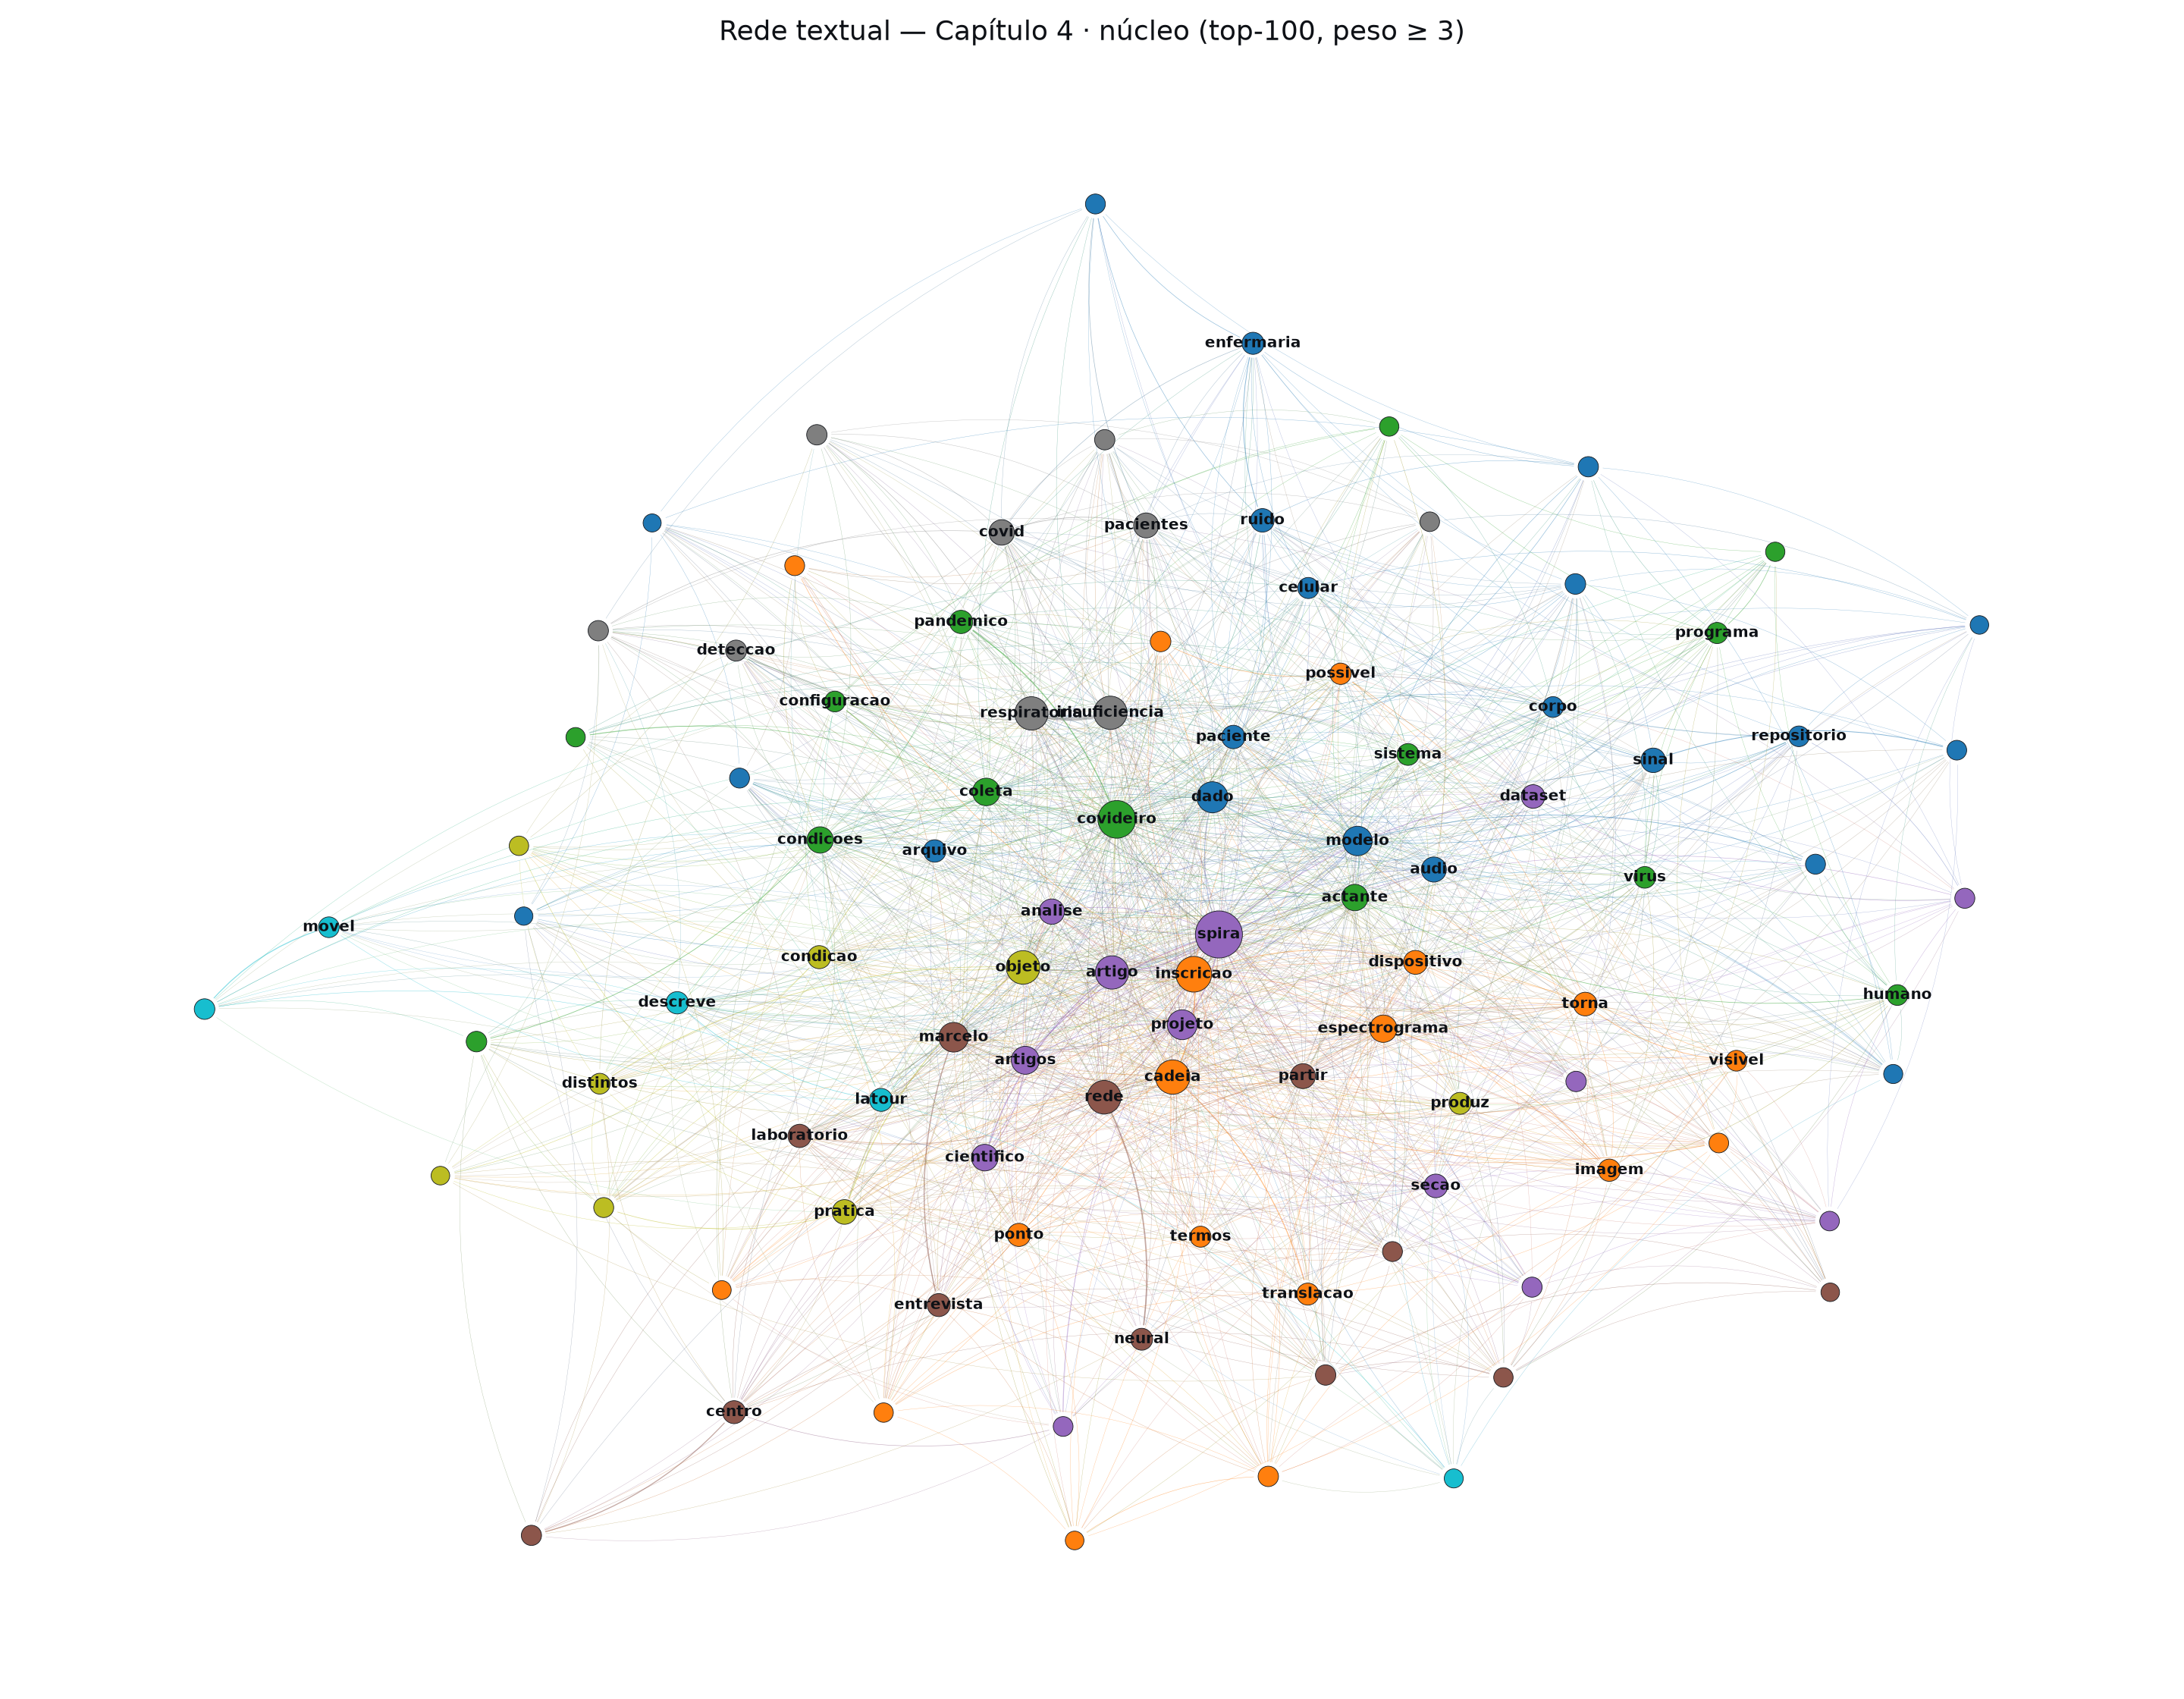
\includegraphics[width=1.0\textwidth,keepaspectratio]{figuras/cap.4/infranodus_cap4_focus.png}
\caption[Núcleo da rede textual do capítulo~\ref{capitulo4} (análise de rede textual)]{Núcleo da rede textual do capítulo~\ref{capitulo4} (análise de rede textual). Os nós são os 100 termos com maior \textit{degree} ponderado; o tamanho do nó é proporcional ao \textit{degree}; a cor indica a comunidade detectada por Louvain ponderado; arestas com peso $\geq 3$. Comparada à figura~\ref{fig:infranodus-cap4-network}, esta vista retém apenas o esqueleto semântico do capítulo, ou seja, os conceitos mais centrais e suas conexões fortes, sem a periferia. Versão de alta resolução, arquivo \texttt{.gexf} para o \texttt{Gephi} e relatório completo disponíveis em \texttt{infranodus/} no repositório \url{https://github.com/julianehelanski/tecno-etnografia-centro-ia}.}
\label{fig:infranodus-cap4-focus}
\end{figure}

\begin{figure}[!htb]
\centering
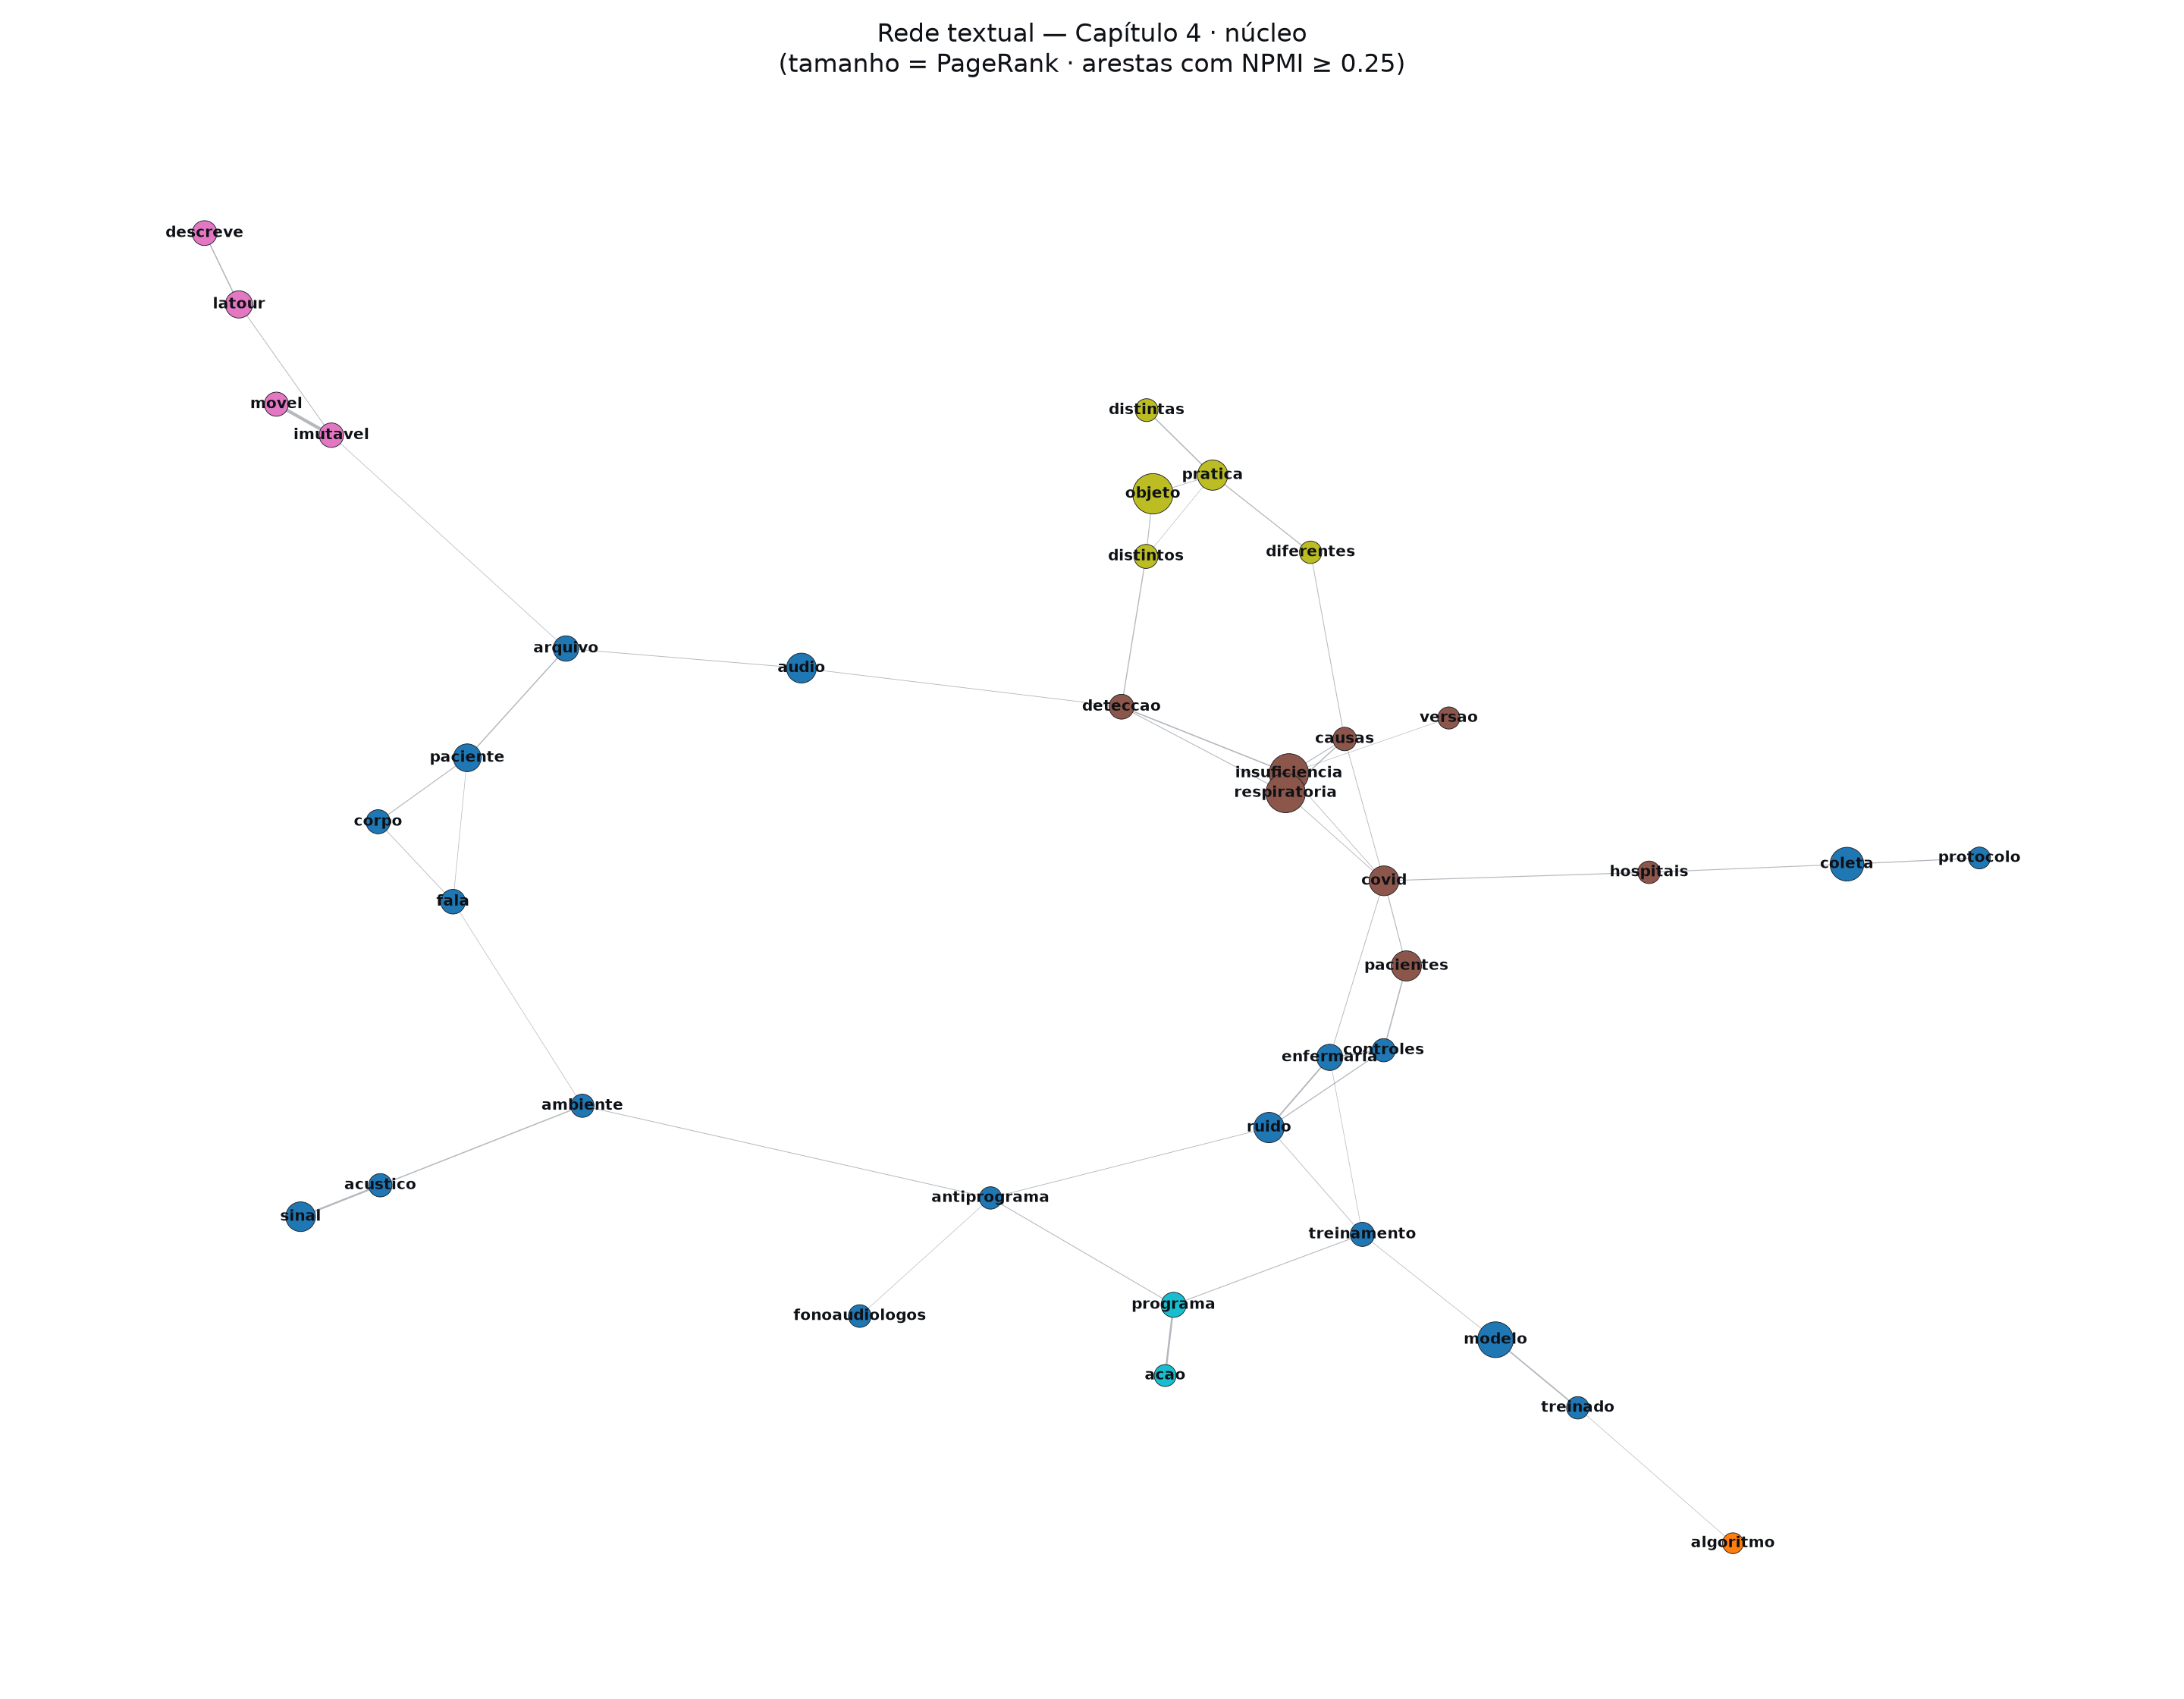
\includegraphics[width=1.0\textwidth,keepaspectratio]{figuras/cap.4/infranodus_cap4_focus_pmi.png}
\caption[Núcleo da rede textual do capítulo~\ref{capitulo4} ponderado por PageRank e NPMI]{Núcleo da rede textual do capítulo~\ref{capitulo4}, ranqueado por critérios informacionais em vez de frequentistas. Os mesmos 100 nós da figura~\ref{fig:infranodus-cap4-focus} são exibidos, mas o tamanho passa a ser proporcional ao \textit{PageRank} (centralidade na rede, em vez de contagem bruta) e as arestas são filtradas pelo \textit{Normalized Pointwise Mutual Information} (NPMI~$\geq 0{,}25$), retendo apenas co-ocorrências surpreendentes dadas as frequências marginais de cada termo. A cor mantém a comunidade Louvain. Esta vista promove conceitos pouco frequentes e estrategicamente posicionados, e deprime termos onipresentes cuja associação com qualquer outro é trivial, funcionando como contraponto à leitura puramente frequentista. Métricas e arquivo \texttt{.gexf} em \texttt{infranodus/} no repositório \url{https://github.com/julianehelanski/tecno-etnografia-centro-ia}.}
\label{fig:infranodus-cap4-pmi}
\end{figure}

\begin{figure}[!htb]
\centering
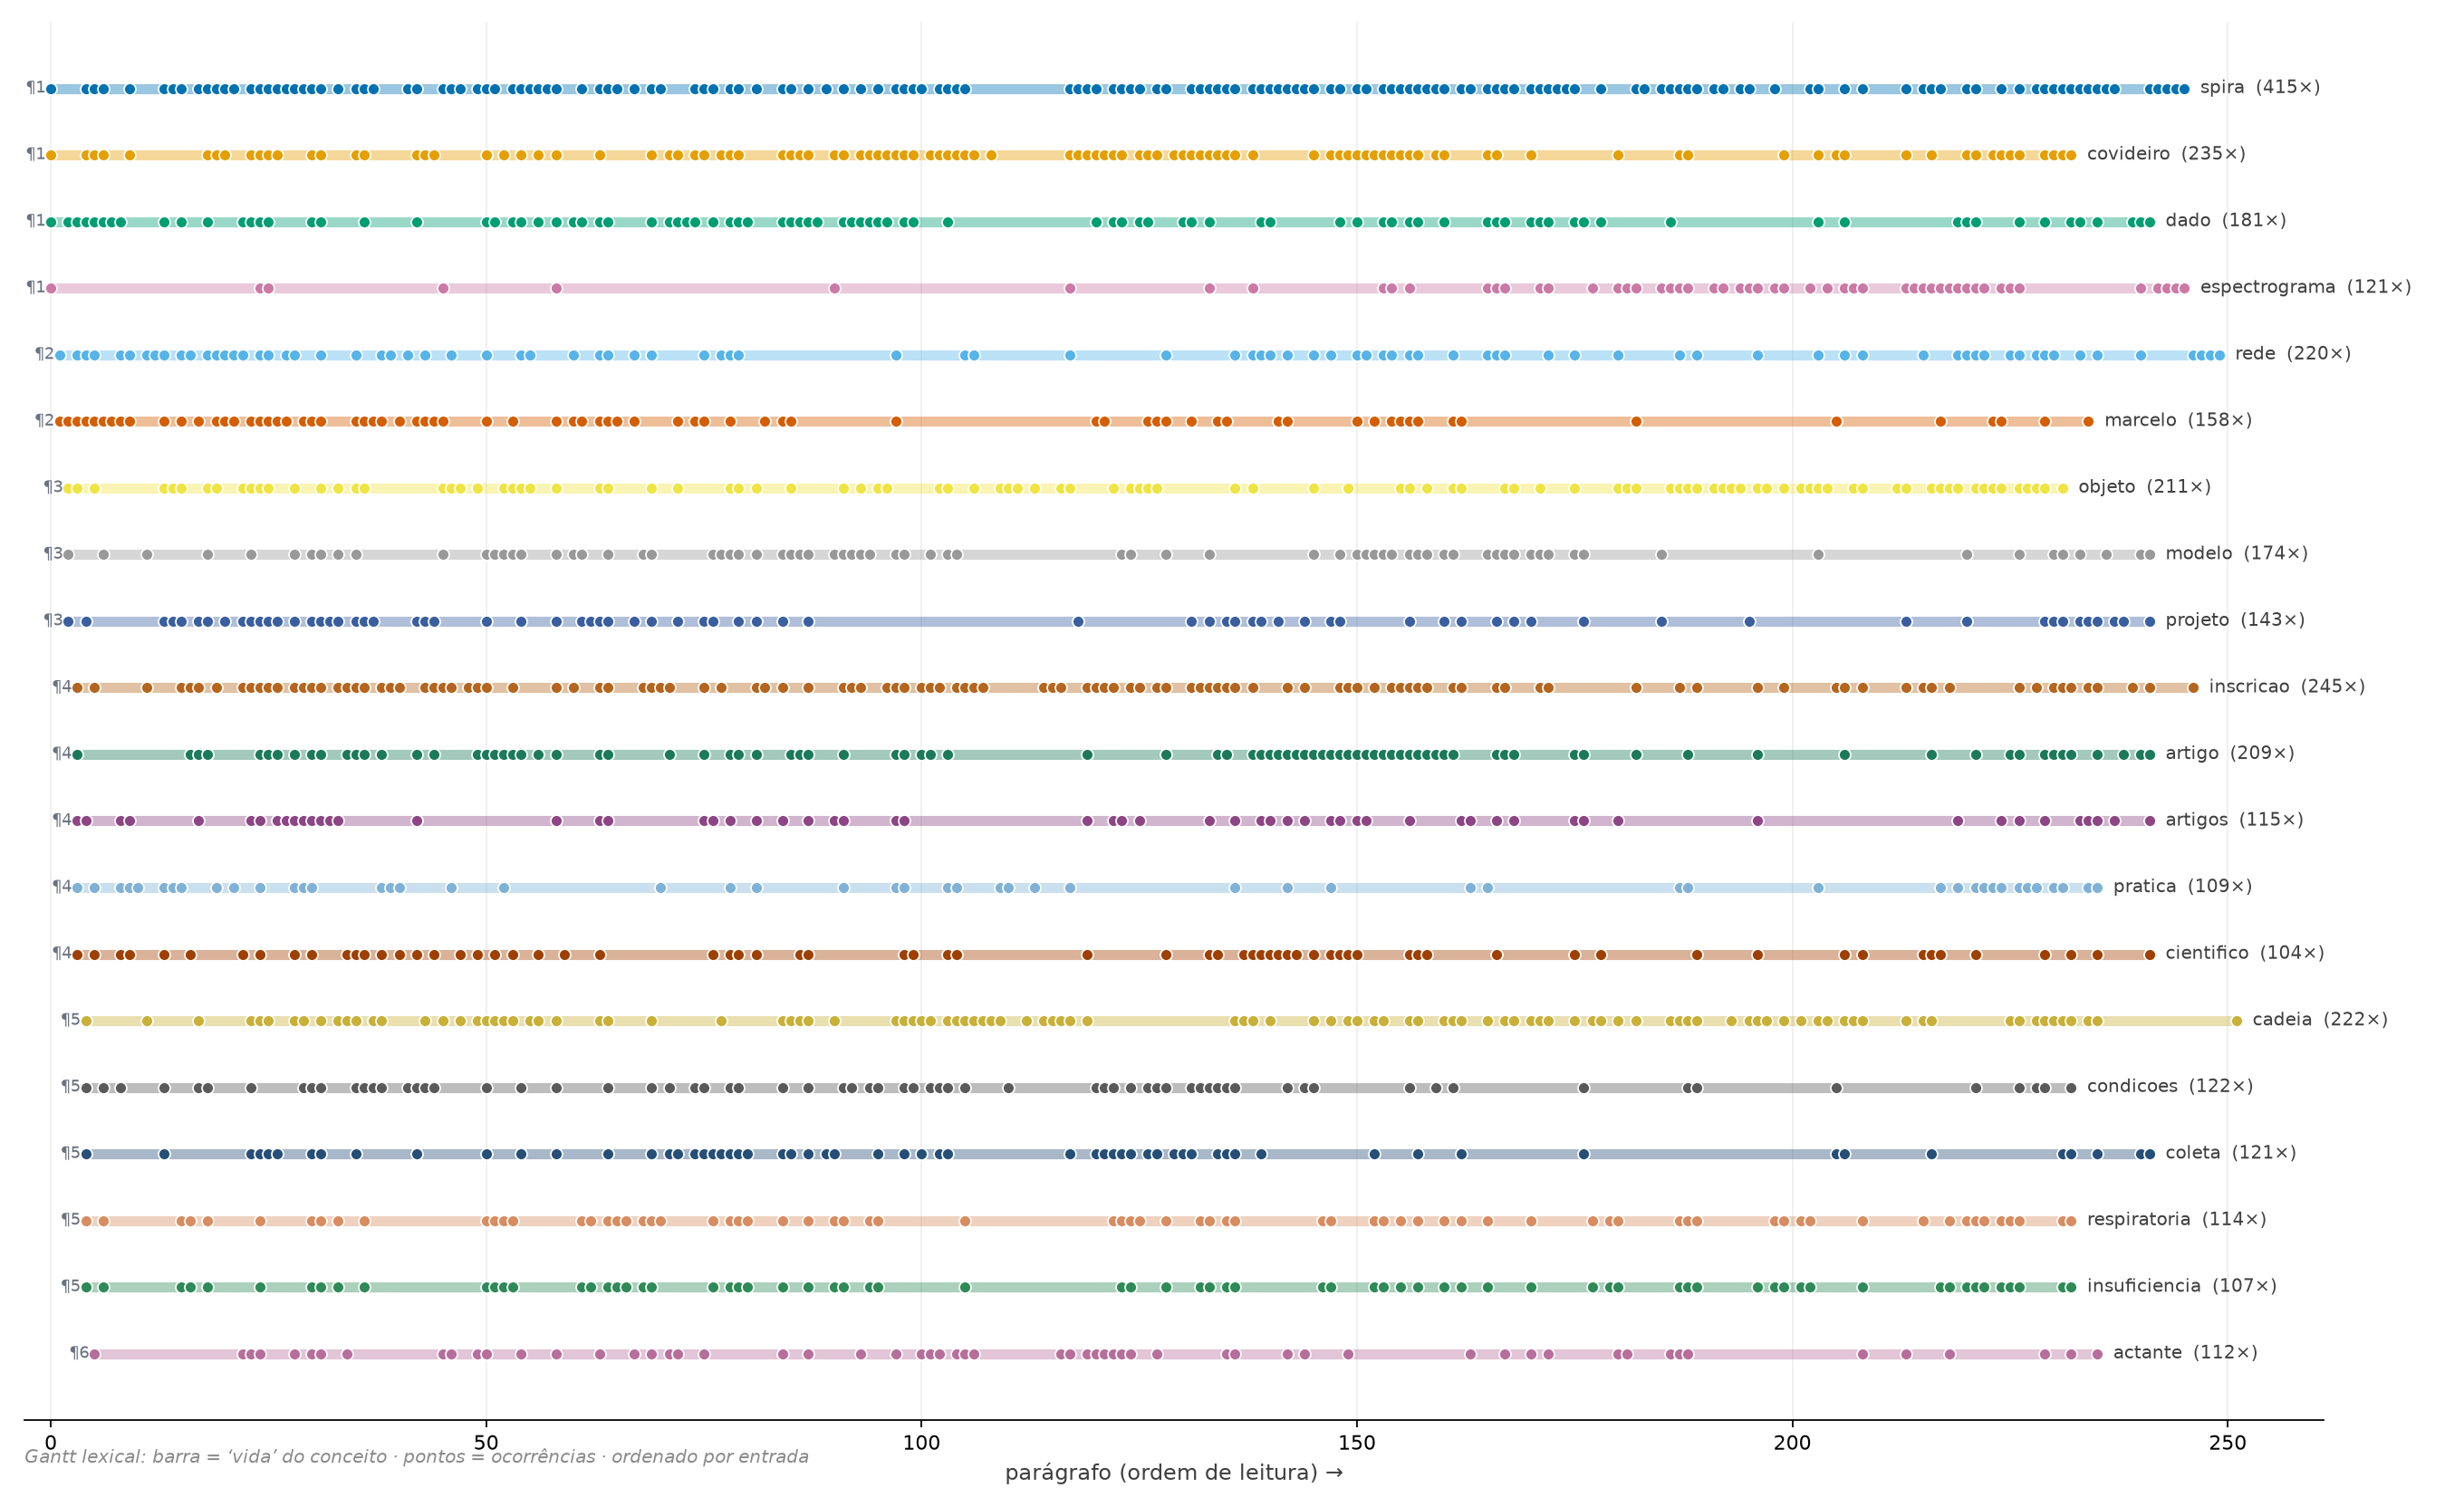
\includegraphics[width=1.0\textwidth,keepaspectratio]{figuras/cap.4/trajectory_gantt.png}
\caption[Gantt lexical do capítulo~\ref{capitulo4}: entrada, persistência e saída dos conceitos]{Gantt lexical do capítulo~\ref{capitulo4}. Cada linha corresponde a um dos 20 conceitos de maior frequência, excluídos termos genéricos e o marcador \texttt{claude}; o eixo horizontal é a ordem de leitura em parágrafos. A barra colorida marca a vida do conceito no capítulo, do parágrafo de primeira aparição (rótulo \P\textit{n}) ao último; os pontos sobre a barra indicam cada ocorrência; o número entre parênteses à direita é a contagem total. As linhas estão ordenadas por parágrafo de entrada, evidenciando a sequência em que cada noção é convocada e por quanto tempo permanece em circulação. Gerado pelo \textit{script} \texttt{narrative\_trajectory.py}, disponível em \url{https://github.com/julianehelanski/tecno-etnografia-centro-ia/tree/main/infranodus}.}
\label{fig:trajectory-cap4-gantt}
\end{figure}

\begin{figure}[!htb]
\centering
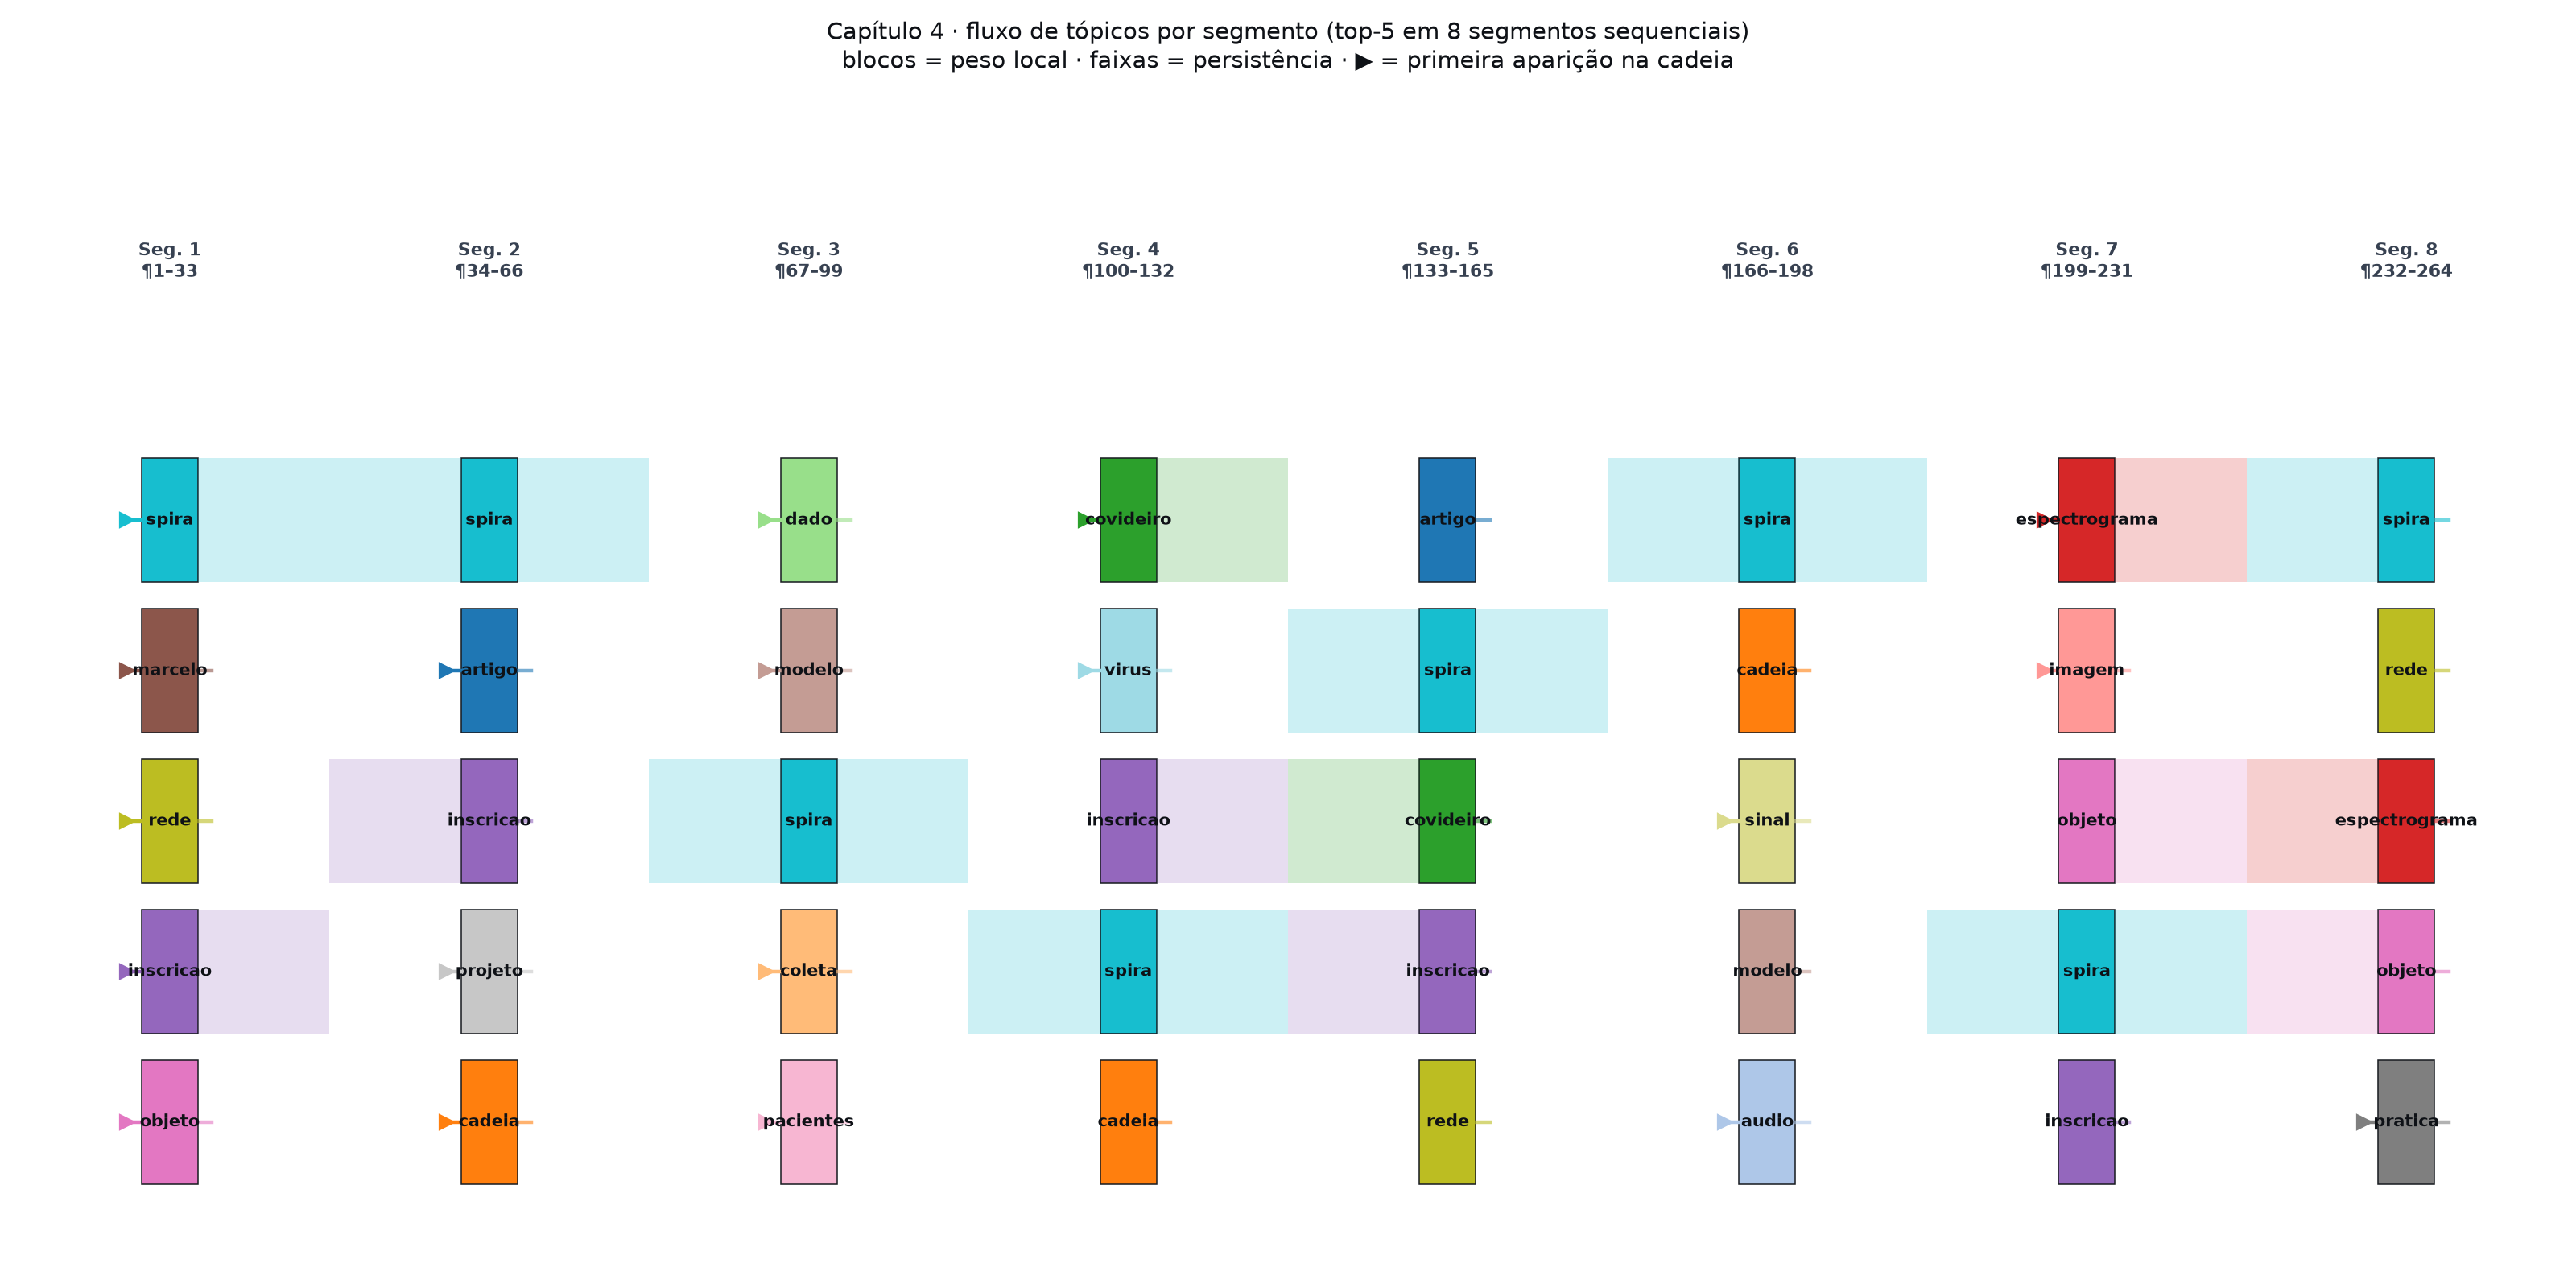
\includegraphics[width=1.0\textwidth,keepaspectratio]{figuras/cap.4/trajectory_alluvial.png}
\caption[Fluxo aluvial de tópicos ao longo do capítulo~\ref{capitulo4}]{Fluxo aluvial do capítulo~\ref{capitulo4}. O capítulo é particionado em 8 segmentos sequenciais de igual extensão em parágrafos (rótulos \P\textit{n}--\P\textit{m} no topo); em cada segmento são listados os 5 termos de maior frequência local (blocos coloridos, com a posição vertical refletindo o \textit{ranking} dentro do segmento). Faixas translúcidas conectam um termo a si mesmo entre segmentos adjacentes quando ele persiste no \textit{top}-5, materializando continuidades temáticas; setas $\blacktriangleright$ assinalam a primeira aparição de um conceito na cadeia. A figura responde à pergunta \enquote{o que se liga a quê ao longo do capítulo} e torna visíveis tanto os tópicos persistentes quanto as entradas tardias e saídas precoces. Gerado pelo \textit{script} \texttt{narrative\_trajectory.py}, disponível em \url{https://github.com/julianehelanski/tecno-etnografia-centro-ia/tree/main/infranodus}.}
\label{fig:trajectory-cap4-alluvial}
\end{figure}

\begin{figure}[!htb]
\centering
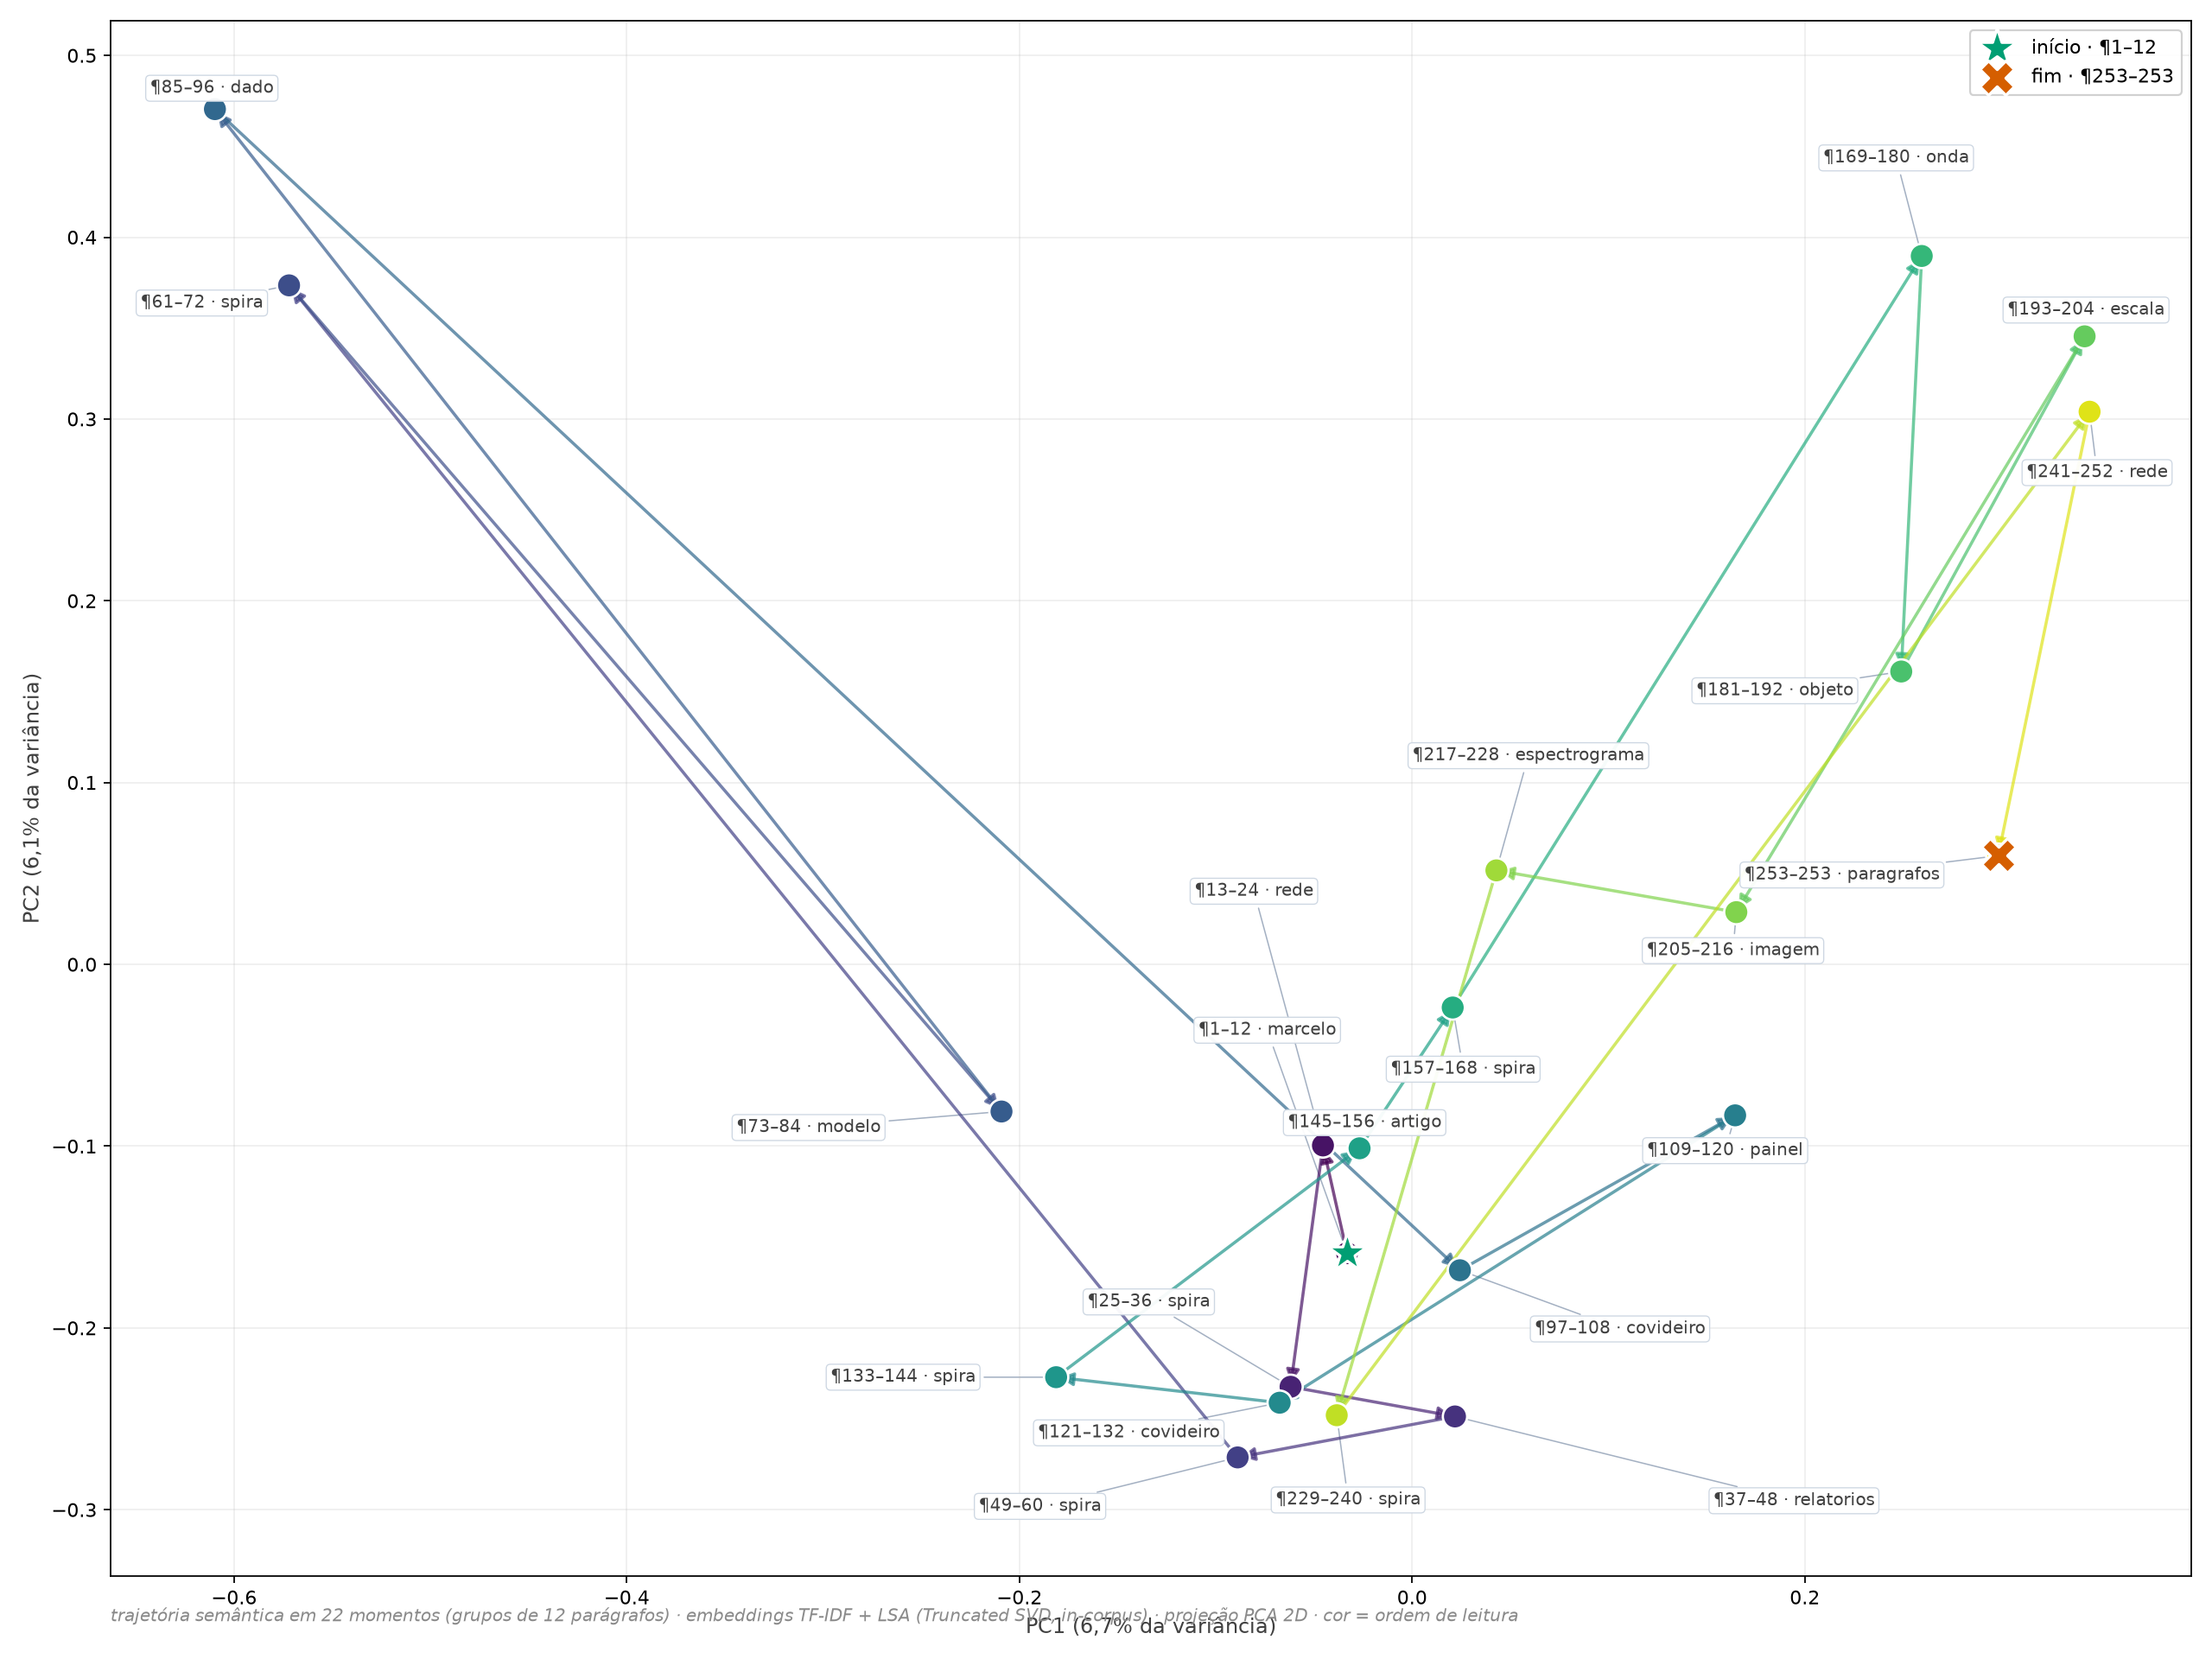
\includegraphics[width=1.0\textwidth,keepaspectratio]{figuras/cap.4/trajectory_semantic.png}
\caption[Trajetória semântica do capítulo~\ref{capitulo4}]{Trajetória semântica do capítulo~\ref{capitulo4}. Os parágrafos são agrupados em \textit{momentos} de 5 parágrafos consecutivos; cada momento é vetorizado por \textit{TF-IDF} (unigramas e bigramas) seguido de redução por \textit{Truncated SVD} (\textit{Latent Semantic Analysis} \textit{in-corpus}, \textit{fallback} usado quando o \textit{sentence-transformer} multilíngue não está disponível) e projetado em duas dimensões por PCA. Cada ponto é um momento, rotulado com o intervalo de parágrafos e o termo dominante; as setas seguem a ordem de leitura, com gradiente \textit{viridis} do início ($\star$ verde) ao fim ($\times$ vermelho). Distâncias no plano aproximam dissimilaridade lexical entre momentos; deslocamentos longos indicam mudanças temáticas, voltas curtas indicam retomada de campo semântico já visitado. O percentual de variância explicada por cada eixo aparece nos rótulos. Gerado pelo \textit{script} \texttt{narrative\_trajectory.py}, disponível em \url{https://github.com/julianehelanski/tecno-etnografia-centro-ia/tree/main/infranodus}.}
\label{fig:trajectory-cap4-semantic}
\end{figure}